%:Clase del documento
\documentclass[11pt,twoside,notitlepage,twocolumn]{article}

%:Paquete de estilos propuesto
%\usepackage{libroETSI}

%:Paquete específico para cargar tikz (y sus librerías) y pgfplots
%\usepackage{dtsc-creafig}

%:Paquete para notaciones específicas
%\usepackage{notacion}

%:Paquete para incorporar aspectos concretos de la edición
%\usepackage{edicionPFC}

%:Estas líneas de código son INNECESARIAS excepto para mostrar determinadas características en este manual. Pueden eliminarse o comentarse sin ningún problema.
%Se usan para compilar el capítulo estilolibroetsi.tex
%\usepackage[final]{showexpl}
%\lstset{explpreset={frame=none,rframe={}, numbers=none,numbersep=3pt, columns=flexible,language={[LaTeX]TeX},basicstyle=\ttfamily,keywordstyle=\color{blue}}}%numberstyle=\tiny,

%:Para modificar fácilmente la fuente del texto.
\makeatletter
\usepackage[utf8]{inputenc}
\usepackage[spanish]{babel}
\usepackage{hyperref}
\hypersetup{
%  	bookmarks=true, %Already used warning
      bookmarksnumbered=false,
      bookmarksopen=false,	
      unicode = true,
	colorlinks=true,
	linktoc=all,
% 	hyperfootnotes=true, %Already used warning
%	urlbordercolor=black,
	plainpages=false,
	pdfpagemode=UseOutlines,
	pdfview=FitH,
	pdfstartview=FitH,
	linkcolor=blue,
	breaklinks=true,
	citecolor=blue,
      anchorcolor=black,
	urlcolor=blue,
	pdfdisplaydoctitle=true
	}
\usepackage{lmodern}
\usepackage{amsmath}
\usepackage{glossaries}
\usepackage{graphicx}
\usepackage{listings}
\usepackage[usenames,dvipsnames]{xcolor}

\renewcommand{\lstlistingname}{Código}

\definecolor{delim}{RGB}{20,105,176}
\colorlet{numb}{magenta!60!black}
\colorlet{punct}{red!60!black}

\lstdefinelanguage{json}{
    literate=
     *{0}{{{\color{numb}0}}}{1}
      {1}{{{\color{numb}1}}}{1}
      {2}{{{\color{numb}2}}}{1}
      {3}{{{\color{numb}3}}}{1}
      {4}{{{\color{numb}4}}}{1}
      {5}{{{\color{numb}5}}}{1}
      {6}{{{\color{numb}6}}}{1}
      {7}{{{\color{numb}7}}}{1}
      {8}{{{\color{numb}8}}}{1}
      {9}{{{\color{numb}9}}}{1}
      {:}{{{\color{punct}{:}}}}{1}
      {,}{{{\color{punct}{,}}}}{1}
      {\{}{{{\color{delim}{\{}}}}{1}
      {\}}{{{\color{delim}{\}}}}}{1}
      {[}{{{\color{delim}{[}}}}{1}
      {]}{{{\color{delim}{]}}}}{1},
}

\newacronym[type=main]{DoS}{DoS}{Denial of Service}
\newacronym[type=main]{DDoS}{DDoS}{Distributed DoS}
\newacronym[type=main]{SO}{SO}{Sistema Operativo}
\newacronym[type=main]{IP}{IP}{Internet Protocol}
\newacronym[type=main]{IPv6}{IPv6}{IP versión 6}
\newglossaryentry{MAC}
{
  name=Medium Access Control,
  description={El control de acceso al medio permite sincronizar el acceso a un enlace entre varios nodos. La dirección 
MAC es la que usa el dispositivo del nodo para identificarse en el enlace o medio compartido}
}
\newacronym[type=main]{ARP}{ARP}{Address Resolution Protocol}
\newacronym[type=main]{TCP}{TCP}{Transmission Control Protocol}
\newacronym[type=main]{UDP}{UCP}{User Datagram Protocol}
\newacronym[type=main]{ICMP}{ICMP}{Internet Control Message Protocol}
\newacronym[type=main]{HTTP}{HTTP}{Hyper Text Transfer Protocol}
\newacronym[type=main]{ITU-T}{ITU-T}{International Telecommunications Union}
\newacronym[type=main]{CNSS}{CNSS}{Committee on National Security Systems}
% TODO TCP SYN, TCP ACK
\newacronym[type=main]{OSI}{OSI}{Open System Interconnection}
\newacronym[type=main]{SYN}{SYN}{Synchronize}
\newacronym[type=main]{ACK}{ACK}{Acknowledge}
\newacronym[type=main]{DNS}{DNS}{Domain Name Server}

\newacronym[type=main]{CdP}{CdP}{Control de Procesos}
\newacronym[type=main]{SCP}{SCP}{Sistema de Control de Procesos}
\newacronym[type=main]{CUSUM}{CUSUM}{Cummulative SUM}
\newacronym[type=main]{VI}{VI}{Variable de Interés}
\newacronym[type=main]{OWCD}{OWCD}{One Way Connection Density}
\newacronym[type=main]{PCAP}{PCAP}{Packet CAPture}
\newacronym[type=main]{pthreads}{Pthreads}{POSIX threads}
\newacronym[type=main]{LIFO}{LIFO}{Last In, First Out}
\newacronym[type=main]{IPC}{IPC}{Inter Process Communication}
\newacronym[type=main]{SIGSEGV}{\texttt{SIGSEGV}}{SIGnal SEGment Violation}
\newacronym[type=main]{SIGTSTP}{\texttt{SIGTSTP}}{SIGnal Terminal STOP}
\newacronym[type=main]{SIGALRM}{\texttt{SIGALRM}}{SIGnal ALARM}

\newacronym[type=main]{PFRING}{PF\_RING}{Packet Filter RING}
\newacronym[type=main]{NIC}{NIC}{Network Interface Controller}
\newacronym[type=main]{DMA}{DMA}{Direct Memory Access}
\newacronym[type=main]{NAPI}{NAPI}{New API}
\newacronym[type=main]{libpcap}{libpcap}{Packet CAPture LIBrary}
\newacronym[type=main]{ssh}{ssh}{Secure SHell}
\newacronym[type=main]{mmap}{MMAP}{Memory MAPping}
\newacronym[type=main]{DUT}{DUT}{Device Under Test}
\newglossaryentry{controlador}
{
  name=Controlador,
  description={Módulo del núcleo Linux que maneja la comunicación entre un dispositivo y el software que lo usa}
}
\newglossaryentry{json}
{
  name=JavaScript Object Notation,
  description={JavaScript es un lenguaje de tipado dinámico. En él se pueden declarar objetos con una estructura 
determinada, que no tienen por qué pertenecer a una clase. El lenguaje descriptivo json es el lenguaje de definición de 
dichos objetos}
  symbol={json}
}
\newglossaryentry{netfilter}
{
	name=Netfilter,
	description={Netfilter es la parte ``cortafuegos'' del núcleo Linux. En él, se pueden definir reglas que afectan a la 
recepción, envío y reenvío de paquetes.}
}
\newglossaryentry{socket}
{
	name=socket,
	description={Extremo de una conexión o flujo de paquetes desde el espacio de usuario.}
}

\newacronym[type=main]{IPS}{IPS}{Intrusion Prevention System}
\newacronym[type=main]{API}{API}{Application Programming Interface}


% Formato A4
%\geometry
%{paperheight=297mm,%
%paperwidth=210mm,%
%top=25mm,%
%headsep=8.5mm,%
%includefoot, 
%textheight=240mm, 
%textwidth=150mm, 
%bindingoffset=0mm, 
%twoside}

\usepackage[a4,center]{crop}%para poner las cruces de esquina de página, poner la opción cross
\newcommand{\redborderddos}{RedBorder DDoS}


%:Empieza el documento

\begin{document}
%:Para incluir toda la referencia bibliográfica aunque no se cite, descomente la siguiente línea
%\nocite{*}


%PORTADA
%ver edicionPFC.sty para modificaciones

% @TODO ttitulo
%:Para crear la portada y la portada interior (pagina titular)
\newcommand{\thetitle}{Funcionamiento y estructura de redBorder DDoS}
\newcommand{\theautor}{Eugenio Pérez Martín}
\title{\thetitle} %\mbox evita que se divida una palabra al cambiar de línea
\author{\theautor}

\hypersetup
	{
 	linkcolor=black, %Tocar para poner color en enlaces
	pdfauthor={\theautor},
	pdftitle={\thetitle}, 
	pdfkeywords={Latex, edición, formato de texto}	
	 }

\maketitle

% !TEX root =../LibroTipoETSI.tex
\chapter*{Resumen}
\pagestyle{especial}
\chaptermark{Resumen}
\phantomsection
\addcontentsline{toc}{listasf}{Resumen}

\lettrine[lraise=-0.1, lines=2, loversize=0.2]{E}{n} nuestra Escuela se producen un número considerable de documentos, tantos docentes como investigadores. Nuestros alumnos también contribuyen a esta producción a través de sus trabajos de fin de grado, máster y tesis. El objetivo de este material es facilitar la edición de todos estos documentos y a la vez fomentar nuestra imagen corporativa, facilitando la visibilidad y el reconocimiento de nuestro Centro.

%La hoja de estilo utilizada es una versión de la que el Prof. Payán realizó para un libro que desde hace tiempo viene escribiendo para su asignatura. Con ella se han realizado estas notas, a modo de instrucciones, añadiéndole el diseño de la portada. El diseño de la portada está basado en el que el prof. Fernando García García, de nuestra universidad, hiciera para los libros de la sección de publicación de nuestra Escuela.


\chapter*{Abstract}
\pagestyle{especial}
\chaptermark{Abstract}
\phantomsection
\addcontentsline{toc}{listasf}{Abstract}

\lettrine[lraise=-0.1, lines=2, loversize=0.2]{I}{n} our school there are a considerable number of documents, many teachers and researchers. Our students also contribute to this production through its work in order of degree, master's theses. The aim of this material is easier to edit these documents at the same time promote our corporate image, providing visibility and recognition of our Center. 

...
\emph{-translation by google-}

 

% \chapter*{\notationname}
\pagestyle{especial}
\chaptermark{\notationname}
\phantomsection
\addcontentsline{toc}{listasf}{\notationname}
%\section*{Notación}
%\begin{table}[htbp]
\begin{longtable}{p{3cm}p{8.5cm}}

%$\displaystyle D$ & Tasa de símbolos  (sim/s) \\
%$\displaystyle R_b$ & Tasa binaria (bit/s) \\
%$\displaystyle T$ & Tiempo de símbolo (s) \\
%$\displaystyle T_{b}$ & Tiempo de bit (s) \\
%$W\left( {t} \right)$ & Ruido blanco\\
%$w\left( {t} \right)$ & Función muestra de un ruido blanco\\
%$\displaystyle h_{c}\left( {t} \right)$ & Respuesta impulsiva de un canal LTI continuo en el tiempo\\
%$\displaystyle H_{c}\left( {\omega} \right)$ & Respuesta en frecuencia de un canal LTI continuo en el tiempo\\
%$\displaystyle h_{c}\left( {\tau;t} \right)$ & Respuesta impulsiva de un canal LTV continuo en el tiempo\\
%$\displaystyle H_{c}\left( {\omega;t} \right)$ & Respuesta en frecuencia de un canal LTV continuo en el tiempo\\
%$\displaystyle h_{c}\left( {n} \right)$ & Respuesta impulsiva de un canal LTI discreto en el tiempo\\
%$\displaystyle H_{c}\left( {\Omega} \right)$ & Respuesta en frecuencia de un canal LTI discreto en el tiempo\\
$\RR$ & Cuerpo de los números reales \\
$\CC$ & Cuerpo de los números complejos\\
$\left\| \vc{v} \right\|$ & Norma del vector $\vc{v}$ \\
$\left\langle {\vc{v}, \vc{w}} \right\rangle$ & Producto escalar de los vectores $\vc{v}$ y $\vc{w}$\\
$\left| {\vc{A}} \right|$ &Determinante de la matriz cuadrada $\vc{A}$\\
$\textrm{det}\left( {\vc{A}} \right)$ &Determinante de la matriz (cuadrada) $\vc{A}$\\
$\vc{A}\trs$ & Transpuesto de $\vc{A}$\\
$\vc{A}\inv$ & Inversa de la matriz $\vc{A}$\\
$\vc{A}{\psd}$ & Matriz pseudoinversa de la matriz $\vc{A}$\\
$\vc{A}\her$ & Transpuesto  y conjugado de $\vc{A}$\\
$\vc{A}\cnj$ & Conjugado\\
c.t.p. & En casi todos los puntos\\
c.q.d. & Como queríamos demostrar\\
\ensuremath{\blacksquare}& Como queríamos demostrar\\
\ensuremath{\square}& Fin de la solución\\
e.o.c. & En cualquier otro caso\\
$\e$ & número e\\
$\xp{x}$ & Exponencial compleja\\
$\xppi{x}$ & Exponencial compleja con $2\pi$\\
$\nxp{x}$ & Exponencial compleja negativa\\
$\nxppi{x}$ & Exponencial compleja negativa con $2\pi$\\
$\re$ & Parte real\\
$\im$ & Parte imaginaria\\
$\sen$ & Función seno \\
$\tg$ & Función tangente \\
$\arctg$ & Función arco tangente \\
$\sento{y}{x}$ & Función seno de $x$  elevado a $y$\\
$\costo{y}{x}$ & Función coseno de $x$  elevado a $y$\\
$\sa$ & Función sampling \\
$\sgn$ & Función signo \\
$\rect$ & Función rectángulo \\
$\sinc$ & Función sinc\\
$\pder{y}{x} $ & Derivada parcial de $y$ respecto a $x$\\
$x\gra$ & Notación de grado, $x$ grados.\\
%
%$C_{XY}$& covarianza  de dos variables aleatorias reales $X$ e $Y$\\
%$R_{XY}$& correlación  de dos variables aleatorias reales $X$ e $Y$\\
%$\rho_{XY}$ &Coeficiente de correlación de las variables aleatorias reales $X$  e $Y$\\
%$\vc{Z}$ & Vector aleatorio complejo\\
%$\displaystyle F_{X}\left( {\cdot} \right)$ & Función de distribución de la variable aleatoria $X$ \\
%$\displaystyle f_{X}\left( {\cdot} \right)$ & Función densidad de probabilidad de la variable aleatoria $X$ \\
%$p_{X}\left( {\cdot} \right)$ & Función masa de probabilidad de la variable aleatoria discreta $X$ \\
%
$\Pr\left( {A} \right)$ & Probabilidad del suceso $A$ \\
$\displaystyle E\left[ {X} \right]$ & Valor esperado de la variable aleatoria $X$ \\
$\si{X}$ & Varianza de la variable aleatoria $X$\\
$\sim f_{X}\left( {x} \right)$ & Distribuido siguiendo la función densidad de probabilidad $f_{X}\left( {x} \right)$\\
%
$\gauss{m_{X}}{\si{X}}$ &Distribución gaussiana para la variable aleatoria X, de media $m_{X}$ y varianza $\si{X}$ \\
$\id{n}$ & Matriz identidad de dimensión $n$\\
$\diag{\vc{x}}$ & Matriz diagonal a partir del vector $\vc{x}$\\
$\diag{\vc{A}}$ & Vector diagonal de la matriz $\vc{A}$\\
$\snr$& Signal-to-noise ratio \\
$\mse$ & Minimum square error\\
$\talq$ & Tal que \\
$\eqdef$ & Igual por definición \\
$\norm{\vc{x}}$ & Norma-2 del vector $\vc{x}$\\
$\card{\vc{{A}}}$ & Cardinal, número de elementos del conjunto $\vc{A}$\\
$\xyz{\vc{x}}{i}{n}$ & Elementos $i$, de 1 a $n$, del vector $\vc{x}$\\
%\newcommand{\xyz}[3]{\ensuremath{#1_{#2},#2=1,2,\ldots,#3}}
$\df{x}$& Diferencial de $x$\\
$\le$ & Menor o igual \\
$\ge$ & Mayor o igual \\
$\BL$ & Backslash \\
$\iff$ & Si y sólo si \\
$x=a+3\eqexpl{a=1} 4 $& Igual con explicación \\
$\tfrac{a}{b}$ & Fracción con estilo pequeño, $a/b$ \\
$\inc$ & Incremento \\
$b\ten{a}$ & Formato científico \\
$\tendsub{x}$ & Tiende, con x \\
$\ord$ & Orden\\
$\tm$ & Trade Mark\\
$\E[x]$ & Esperanza matemática de x\\
$\covm{\vc{x}}$ & Matriz de covarianza de $\vc{x}$\\
$\corrm{\vc{x}}$ & Matriz de correlación de $\vc{x}$\\
$\si{x}$ & Varianza de x \\


\end{longtable}
\newpage
%\end{table}
%


%\phantomsection
%\addcontentsline{toc}{listasf}{Acrónimos}
%\section*{Acrónimos}
%\begin{table}[htbp]
%\begin{tabular}{p{2cm}p{10cm}}
%Escuela Técnica Superior de In
%LTI & Lineal Invariante con el Tiempo \\
%LTV& Lineal Variable con el Tiempo\\
%AWGN& Ruido blanco gaussiano aditivo\\
%DMS& Fuente discreta sin memoria\\
%AEP& Propiedad de equipartición asintótica\\
%WLLN& Ley Débil de los Grandes Números\\
%DMC& Canal Discreto sin Memoria\\
%BSC& Canal Simétrico Binario\\
%BEC& Canal Binario con Borrado\\
%\end{tabular}
%\end{table}


%\nota{El libro de Lapidoth tiene una excelente recopilación.} %No incluir si no se quiere, comentándolo

%:Los diferentes capítulos, en carpetas separadas
%
% !TEX root =../LibroTipoETSI.tex
%El anterior comando permite compilar este documento llamando al documento raíz
\chapter{Guía de Uso}\label{chp-01}
\epigraph{The fundamental problem of communication is that of reproducing at one point either exactly or approximately a message selected at another point.}{Claude Shannon, 1948}

%\lettrine[lraise=0.7, lines=1, loversize=-0.25]{E}{n}
\lettrine[lraise=-0.1, lines=2, loversize=0.2]{E}{n} este capítulo vamos a describir las partes de las que consta un documento tipo, cómo deben interpretarse los diferentes comandos que se han definido para su confección, los \indexit{paquetes} (conjunto de sentencias de \LaTeX\ escritas y desarrolladas por diversos autores) que se han cargados y el porqué de los mismos, elecciones realizadas en cuanto a la edición, el porqué de determinadas fuentes, etc. 

Hay mucho de elección personal en lo que sigue y únicamente se justifica desde el gusto personal de quienes escribimos esto. No pretendemos por ello sentar precedentes, obligaciones ni restricciones a quien desee utilizar este documento. En cualquier caso, esperamos que su lectura sea provechosa para la confección y edición de libros, apuntes de clase, proyectos, etc.

\LaTeX se ha convertido de hecho en el procesador de texto estándar para la edición de documentos científicos. Este libro está escrito precisamente en \LaTeX, haciendo uso de la plantilla que hemos diseñado y al escribir un libro sobre cómo escribir un libro en \LaTeX\  y cómo hacer uso de esta plantilla, estamos entrando muchas veces en una redundancia evidente.

Estas páginas no constituyen un manual de \LaTeX,  ni lo pretendemos, ya que existen incontables y buenas referencias sobre este tema. El objetivo es describir los aspectos formales que deseamos se puedan incorporar a cualquier texto producido en la Escuela.  También, como la mayoría de nuestra producción científica utiliza ampliamente las fórmulas matemáticas, incluimos algunos consejos sobre la escritura de las mismas, para lo que hemos utilizado las notas preparadas en \cite{moser}. Asimismo resulta muy interesante el libro \cite{gratzer}.

Por último, puesto que los ficheros fuentes de este documento están disponibles, esperamos que los mismos faciliten la utilización de los distintos elementos de edición.

\section{Cómo usar los  estilos de documento de la ETSI}\label{sec-00}

Una de las bondades del \LaTeX\ es que una vez definido el estilo, formado por un conjunto de paquetes y adaptaciones de los mismos, la escritura de un texto se reduce a dominar una serie de comandos. En nuestro caso, se presenta este documento como ejemplo de uso de estos comandos. En este capítulo encontrará detalles técnicos sobre la estructura del documento y una breve introducción sobre algunos de los elementos del estilo diseñado, puesto que en el Capítulo \ref{chap:estilo} se estudian detalladamente todos sus componentes. También encontrará instrucciones de cómo compilar el documento. Para usar esta hoja de estilo, se recomienda leer el Capítulo \ref{chap:CAPEJ} y Capítulo \ref{chap:CAPPB} como ejemplos de capítulos donde se incluyen la mayoría de los comandos que pueden ser de utilidad en la redacción de un texto técnico. 

El archivo \ttcolor{libroTipoETSI.tex} es el archivo principal, que tiene una serie de comandos para incluir las distintas partes que se necesiten. Muchas de estas partes se han incluido separadamente en carpetas, por comodidad. Este archivo lo hemos modificado levemente para utilizarlo como formato para proyecto fin de carrera/grado/máster. El resultado se incluye en un fichero con nombre \ttcolor{pfcTipoETSI.tex}. Y también se incluye un formato para tesis \ttcolor{tesisTipoETSI.tex}

Los datos necesarios para generar la cubierta y demás hojas iniciales se incluyen al comienzo de estos ficheros: el título del proyecto, autores, el nombre del departamento, etc. Si necesita retocar la cubierta  (por ejemplo el ancho de la imagen utilizada)  tendrá que modificar directamente el fichero \ttcolor{edicionLibro.sty}, que es el fichero al que se llama para generarla. Si quiere, también, puede retocar la imagen de fondo. Todo esto se explica en un apartado más adelante. Para los restantes tipos de documentos, estas modificaciones hay que hacerlas en los ficheros \ttcolor{edicionPFC.tex} y \ttcolor{edicionTesis.sty}.

Así, para empezar a utilizar este documento, basta que empiece modificando los ficheros \ttcolor{libroTipoETSI.tex} (ó \ttcolor{pfcTipoETSI.tex}, {tesisTipoETSI.tex} ) y cada uno de los ficheros que éste incluya, bien introduciendo los cambios oportunos, bien eliminándolos (puede simplemente comentar la línea correspondiente).

Una vez modificado, el segundo paso es compilarlo. Debe elegir el tipo de formato, A4 ó libro. Por defecto, \ttcolor{libroTipoETSI.tex} y \ttcolor{tesisTipoETSI.tex}  están en formato libro y \ttcolor{pfcTipoETSI.tex} en A4. Para cambiar cualquiera de ellos, debe buscar el comando \ttcolorc{geometry} dentro del fichero  \ttcolor{libroTipoETSI.tex} y establecer los parámetros correspondientes o bien tendrá que comentar la correspondiente a tamaño libro para descomentar la correspondiente al formato A4, o viceversa. También, hay un conjunto de comandos más adelante que están comentados y que permiten presentar el texto en formato \ind{manuscrito}, con un interlineado distinto prefijado a $1.5$ líneas. 

\subsection{Compilación}

\subsubsection{{Macintosh}\tsp{\textregistered}}
Este trabajo se ha desarrollado en un ordenador \ind{Macintosh}\tsp{\textregistered}. Como iremos viendo, \LaTeX\ consta de un elevado número de programas y existen un conjunto de distribuciones que facilitan su uso. Nosotros hemos elegido una de las versiones más utilizadas, Tex-Live, versión 2013, \url{http://mirror.ctan.org/systems/mac/mactex/MacTeX.pkg}, en su versión para el sistema operativo Mac OSx\tsp{\textregistered}. Para la bibliografía  se ha utilizado \ind{BibTex}. 

Como editor de ficheros y compilador hemos usado \ind{TeXShop}\tsp{\textregistered}. Puede usar pdflatexmk para compilar, que va bien y genera directamente la bibliografía y los índices de palabra y glosarios. Aquí se recomienda utilizar el comando \ttcolor{lualatexmk}, que es un determinado motor \ind{engine} de TeXShop\tsp{\textregistered}. Si no lo ve en la lista de opciones de componer, vaya a las librerías de usuario y en la carpeta TeXShop/Engines saque lualatexmk.engine de la subcarpeta Inactive. Si no quiere complicarse,  En todo caso, puede usar también \LaTeX\ y BibTeX. Pero si compila con \LaTeX\ y luego desea usar Lua\LaTeX mk, deberá borrar todos los archivos auxiliares, menos los archivos con la extensión \ttcolor{.tex} y \ttcolor{.bib} que se corresponden, respectivamente, al fichero fuente de \LaTeX\ y de la bibliografía.

Si utiliza un índice de palabras y un glosario, vaya a la sección correspondiente para ver cómo generarlos.

\subsubsection{Windows\tsp{\textregistered}}

Existen versiones de la distribución Tex-Live para las diferentes versiones de Windows\tsp{\textregistered} y en la dirección señalada anteriormente pueden encontrarse instrucciones para su instalación en este y restantes sistemas operativos. No se ha probado con el conjunto MikTeX, pero probablemente funcionaría igualmente.

Como editor y compilador de ficheros hemos optado por \ind{TexMaker}\tsp{\textregistered}, igualmente con una codificación UTF-8. Hasta donde conocemos, el editor \indexit{Winedt}\tsp{\textregistered} no reconoce esta codificación. Para la bibliografía se ha utilizado BibTeX. Para compilar tendrá que o bien usar LatexMk ó PDFLaTeX. No olvide seleccionar la opción UTF-8 en ``Opciones'' en el menú, y luego en la ventana emergente pulsando Editor y allí en el campo Codificación de editor. 

Si utiliza un índice de palabras y un glosario, vaya a la sección correspondiente para ver cómo generarlos.

\subsubsection{Lyx}

En \url{http://www.lyx.org/}, el lector puede encontrar una opción alternativa a la forma de trabajo tradicional de \LaTeX, tanto en Windows\tsp{\textregistered} como en MacOS\tsp{\textregistered}. En este entorno, uno puede trabajar con un entorno de edición gráfico, tal como se trabaja por ejemplo en Microsoft Word\tsp{\textregistered}. Una vez terminado el documento, es relativamente sencillo compilarlo en \LaTeX. De hecho, hemos realizado algunas pruebas positivas en este sentido. En cualquier caso se recomienda no usar nombres de archivo con ñ, tildes, o espacios. 

\subsection{Texto en inglés}
Si escribe el texto en inglés, deberá de cambiar el idioma en la opción de Babel, uno de los paquetes claves para la escritura en \LaTeX. En el fichero \ttcolor{libroTipoETSI.sty}, se debe buscar la línea que comienza por \comando{usepackage}\ttcolor{[spanish, english...]\{babel\} } y seguir con las instrucciones correspondientes. Esto hará que automáticamente los nombres de secciones, apartados, teoremas, ejemplos, etc, aparezcan en inglés. 

\section{Elementos básicos de un libro}
%
En este capítulo describimos los puntos que pueden incluirse con el formato propuesto. En primer lugar, la longitud de un libro, en general, justifica su separación en partes. Una posibilidad es que un libro esté dividido en Partes y esta a su vez en Capítulos. Y por último, a veces existen Apéndices que se incorporan cuando han acabado los capítulos. En nuestro caso sólo hemos considerado la posibilidad de dividir el libro en capítulos y apéndices. Además, existen un conjunto de elementos como dedicatoria, prefacio, agradecimientos, portada, etc, que también son partes que se han tenido en cuenta. 

Se ha optado por estructurar los ficheros fuente de este texto en carpetas que cuelgan de una principal en la que se encuentra alojada el fichero principal que las utiliza o agrupa. En nuestro caso, por ejemplo, el fichero principal se denomina \ttcolor{libroTipoETSI.tex} (ó \ttcolor{pfcTipoETSI.tex}, \ttcolor{tesisTipoETSI.tex}) y colgadas de la carpeta que lo contiene se encuentran las carpetas \ttcolor{introducción}, \ttcolor{dedicatoria}, ..., \ttcolor{capitulolibroETSI}\footnote{Tenga en cuenta que en algunas imprentas pueden cobrar más por copias de hojas en color. Para ello asegúrese de que utiliza los colores convenientemente, y -en su caso- que los grises lo son de verdad.}, etc. De alguna forma, este fichero principal es el esqueleto que describe cómo está formado el libro.

En un nivel de descripción diferente, podríamos considerar que un libro se encuentra dividido en cubierta, páginas de cortesía, portada, página de título y trasera de la página de título, elementos antes del cuerpo del libro, tales como agradecimientos, prefacio, índices, etc, el cuerpo del libro en sí, dividido en capítulos y esto a su vez en secciones, subsecciones, subsubsecciones, %parágrafos,
subcapítulos, apéndices y, por último, la parte del libro después del cuerpo, que agruparía elementos tales cómo la lista de figuras del libro, la bibliografía, el índice, etc. En \LaTeX\ estas tres partes se dividen con los comandos  \ttcolorc{frontmatter}, \ttcolorc{mainmatter} y \ttcolorc{backmatter}. Estos comandos, y muchos otros, nos permiten describir formalmente el contenido del libro, tal cómo se realiza en el fichero \ttcolor{libroTipoETSI.tex}. Este fichero, como hemos dicho, constituye el esquema de nuestro libro y entender por qué están allí cada una de sus partes es de interés, que no imprescindible, de cara a poder confeccionar un texto. 
%Veamos sus diferentes partes.

\section{Clase de documento}
El comando \comandos{documentclass[paper=a4,10pt, twoside]}{scrbook} o uno similar es el primer comando que aparecerá en cualquier documento de \LaTeX. La parte importante del mismo es \ttcolor{scrbook} y hace referencia a la elección de una  clase de documento tipo libro pero tal como se define en el conjunto de programas denominado \ttcolor{Koma}. Se ha elegido este tipo de documento fundamentalmente por generar un tipo de texto próximo a los estándares europeos, en contraposición con la clase estándar \ttcolor{book}. Una posible alternativa consistiría en la utilización de la clase \ttcolor{Memoir}. En cualquier caso, debido a las posibles modificaciones del conjunto \ttcolor{Koma}, es inmediato sustituir la clase de documento por la standard \ttcolor{book}.

Existen además un conjunto de parámetros, todos los encerrados entre \ttcolor{[...]} que modifican de alguna manera el tipo de documento que vamos a generar. Para entender el significado de cada uno de ellos se puede consultar la referencia \cite{koma}. En cualquier caso, \ttcolor{paper=a4} hace referencia a la dimensión del papel que vamos a utilizar (más adelante diremos algo más acerca de esto), \ttcolor{10pt} establece el tamaño de la fuentes en \ttcolor{puntos tipográficos} y \ttcolor{twoside} nos indica que vamos a generar un documento a doble cara. 

Por último, se han incorporado tres nuevos parámetros: \ttcolor{Myfinal=false}, \ttcolor{Minion=false} y \ttcolor{English=false}. Mediante el primero, que como todos ellos también puede tomar el valor \ttcolor{Myfinal=true}, se le indica a \LaTeX\ que nos encontramos en la versión final del documento, realizándose con ello una serie de ajustes \emph{finos} en la partición silábica, la separación entre palabras (o incluso un ligero ensanchamiento) que hacen más agradable visualmente el texto generado. 

Mediante el parámetro \ttcolor{Minion=true} ó \ttcolor{Minion=false} se le indica a  \LaTeX\ que utilice o no el paquete \ttcolor{Minion}. Este paquete permite la utilización de una fuente denominada Minion Pro para el texto y el conjunto de símbolos matemáticos que lo acompañan, denominados MnSymbol. No resulta trivial la instalación de este paquete por lo que en general la opción por defecto es su no utilización. No hay que confundir la utilización de la opción \ttcolor{Minion=true} ó \ttcolor{Minion=false} con el uso de la fuente Minion Pro para el texto del documento. Ambas cosas están separadas aunque desde un punto de vista tipográfico no deberían estarlo. Es decir, si queremos elegir una fuente Minion Pro para el texto, lo más acertado sería elegir esa misma fuente para el texto matemático. Esta elección conjunta es la que se activa con \ttcolor{Minion=true}.

Por último, resulta evidente el significado  del parámetro \ttcolor{Englis=false} que también puede ser \ttcolor{English=true}.

\section{Fichero de estilo LibroETSI.sty}
La instrucción que sigue a la declaración de la clase es  \comandos{usepackage}{LibroETSI}. Con ella  cargamos y definimos  las principales características tipográficas y de muy diversa índole que hemos propuesto para el diseño de los documentos de la Escuela. A lo largo del presente documento se irán revelando diversos aspectos del mismo, pero se empieza aquí con una pequeña introducción. En el Capçitulo correspondiente se describen ordenadamente todas sus características. 

Debemos observar antes que nada que es un fichero con la extensión \ttcolor{sty} y siempre debe estar antes del comando \comandos{begin}{document}. En él se cargarán un conjunto de paquetes que hemos considerado necesarios y se definirán un conjunto de comandos que facilitan la escritura del texto. Una buena práctica para escribir un libro o cualquier documento que posea una extensión considerable es agrupar en un fichero como el presentado el conjunto de elementos que necesitamos para su escritura: paquetes y comandos.

\subsection{Paquete Babel}
Como ya hemos dicho, el primer paquete importante (existen otros anteriores, pero de carácter mucho más técnico que otra cosa) es el paquete \ttcolor{babel}, que se carga en nuestro fichero mediante la instrucción 

\comandos{usepackage [english, spanish, es-nosectiondot, es-noindentfirst,\\ es-nolists, activeacute]}{babel}. 

Su papel fundamental es declarar que el texto estará escrito en español, que podemos utilizar sin restricción los acentos (no sería posible en \LaTeX\ si no lo declarásemos como idioma preferente) y que adoptaremos los usos convencionales de mayúsculas, acentos en expresiones matemáticas, etc recomendados por la RAE. A todo esto contribuye también la sentencia \comandos{spanishdecimal}{.}. Ya se ha comentado que intercambiando las palabras english por spanish obtenemos los nombres de capítulo, sección y otros en inglés.

\subsection{Símbolos y fórmulas}
Aunque \LaTeX\ no es sólo un sistema de edición para textos científicos, su aplicación para ellos es prácticamente universal. En el estilo de libro que hemos propuesto, la utilización de las fuentes en los textos matemáticos y el posible uso de diversos símbolos y herramientas propias para los textos científicos está recogido en diversos paquetes, entre los que cabe destacar \comandos{usepackage[cmex10]}{amsmath}, \comandos{usepackage}{amssymb} y \comandos{usepackage}{mathptmx}.

\subsection{Fuentes}
La selección de las fuentes para la edición de cualquier texto no es fácil. En realidad, el diseño tipográfico es todo un arte. Un convenio bastante aceptado es utilizar fuentes con serif para el texto y sin serif para titulares y cabeceras de páginas. Sin embargo, la elección de cualquiera de estas familias de fuentes es prácticamente cuestión de gusto personal y, por que no decirlo, de la moda del momento.

En los primeros tiempos de \LaTeX\ y \TeX\ las posibilidades de elección estaban bastante delimitadas. Sin embargo, con el advenimiento de nuevos métodos y programas, es posible elegir prácticamente cualquier fuente existente para su uso. En cualquier caso, no es un tema trivial ni sencillo, como puede verse en la considerable extensión de todo lo relacionado con las fuentes en nuestra hoja de estilos. Nuestra elección se pone de manifiesto en este texto.

Existen además un conjunto de razones históricas que complican enormemente la elección de la fuente (aunque en realidad habría que hablar de las fuentes) del texto. Si se utiliza como motor de composición Pdf\LaTeX\, la forma más simple de seleccionar las fuentes se realiza mediante comandos específicos como, por ejemplo,  \comandos{usepackage}{tgtermes}, que se encuentra utilizado en el fichero \ttcolor{libroTipoETSI.tex}.  Sin embargo, si se utilizan motores más recientes como \XeLaTeX\ o \LuaLaTeX\, podremos seleccionar cualquier fuente \ttcolor{OTF} o \ttcolor{TTF} que se encuentre en nuestro ordenador. En este caso, tal  como se detalla en un apartado más adelante, este texto propone la utilización de la fuente \ttcolor{Minion Pro} que se encuentra disponible de manera generalizada al haber sido licenciada gratuitamente por \ind{Adobe}\tsp{\textregistered} siempre que se instale el programa gratuito Adobe Reader. 

\subsection{Epígrafes}
En muchos libros, después del título de un capítulo o antes del resumen, o en el lugar que apetezca, se coloca una frase con diversos significados. Esto en \LaTeX\ se consigue con el comando \ttcolorc{epigraph}, para lo cual es necesario que se instale el paquete \comandos{usepackage}{epigraph}. %, cuyo uso se explica en el texto del archivo. 

\subsection{Figuras y tablas}
Una parte importante de cualquier texto son las figuras y tablas que lo acompañan. En \LaTeX\  estos elementos se consideran elementos flotantes y hemos cargado un conjunto de paquetes que facilitan su inclusión y formato.

La inclusión de las figuras se realiza mediante un conjunto de instrucciones que se muestran en  el Código \ref{prg01-01}.

%\begin{micuadro}{Inclusión de una figura}{prg01-01}

\begin{lstlisting}[language=,caption={Inclusión de una figura}, breaklines=true, label=prg01-01]
\begin{figure}[htbp]
\centering
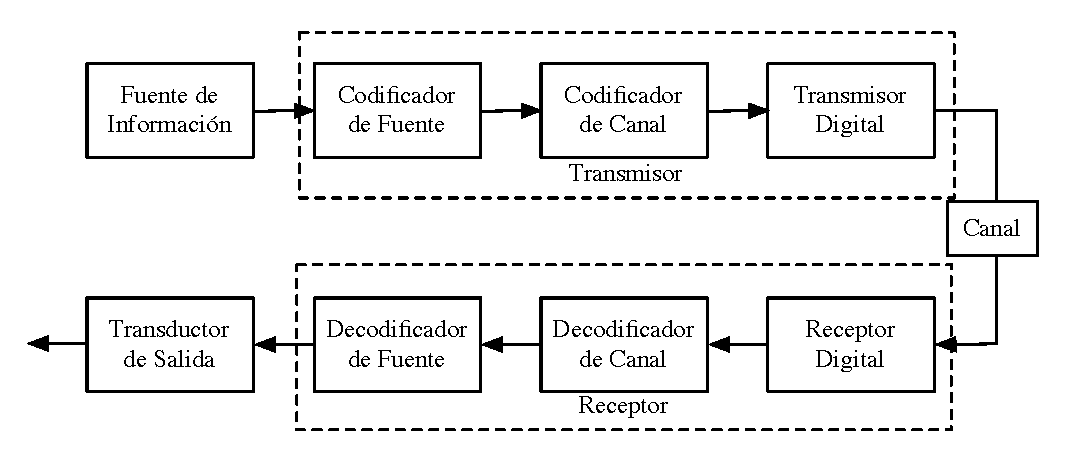
\includegraphics[width=0.95\linewidth]
{introduccion/figuras/fig01-01.pdf}
\caption{Modelo de un sistema de Comunicación Digital I}
\label{fig01-01}
\end{figure}
\end{lstlisting}
%\end{micuadro}

Y el resultado se muestra en la \autoref{fig01-01}.

%
\begin{figure}[htbp]
\centering
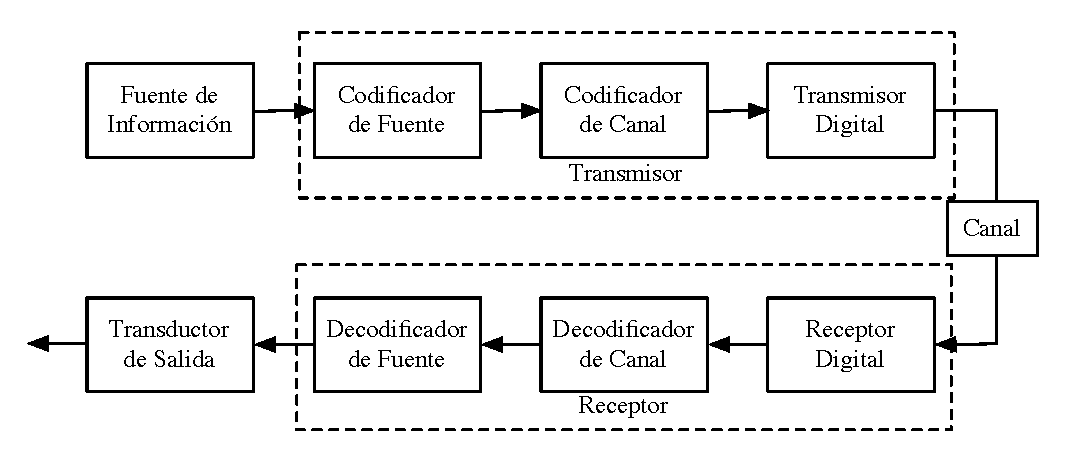
\includegraphics[width=0.95\linewidth]{introduccion/figuras/fig01-01.pdf}
\caption{Modelo de un sistema de Comunicación Digital I}
\label{fig01-01}
\end{figure}
%

Para incluir una tabla utilizamos las instrucciones siguientes:
%\nopagebreak 
\begin{lstlisting}[language=,caption={Inclusión de una tabla}, breaklines=true, label=prg01-02]
\begin{table}[htbp]
	\ttabbox
	{\caption{Tipos de transmisión y frecuencia central} 
	\label{tab2_1}}
		{
		\begin{tabular}{c c}
		\hline
		\rule[-8pt]{0pt}{22pt}{\bf Tipo de Transmisión}&
		 {\bf Frecuencia central de transmisión} \\
		\hline
		\rule{0pt}{14pt}Modem & 100-1800 Hz \\
		Radio AM & 530-1600 kHz \\
		Radio FM & 88-108 MHz \\
		Televisión & 178-216 MHz \\
		Telefonía móvil & 850 MHz-1,8 GHz \\
		Redes inalámbricas &  $2,4$ GHz \\
		Fibra óptica & $2\cdot 10^{14}$ Hz \\
		\hline
		\end{tabular}
		}
\end{table}
\end{lstlisting}

Y el resultado se muestra en la \autoref{tab2-1}.

\begin{table}[htbp]
	\ttabbox
	{\caption{Tipos de transmisión y frecuencia central} \label{tab2-1}}
		{
		\begin{tabular}{c c}
		\hline
		\rule[-8pt]{0pt}{22pt}{\bf Tipo de Transmisión}& {\bf Frecuencia central de transmisión} \\
		\hline
		\rule{0pt}{14pt}Modem & 100-1800 Hz \\
		Radio AM & 530-1600 kHz \\
		Radio FM & 88-108 MHz \\
		Televisión & 178-216 MHz \\
		Telefonía móvil & 850 MHz-$1,8$ GHz \\
		Redes inalámbricas &  $2,4$ GHz \\
		Fibra óptica & $2\cdot 10^{14}$ Hz \\
		\hline
		\end{tabular}
		}
\end{table}

Observemos  que en la parte inferior de las figuras y en la superior de las tablas (esta ha sido nuestra elección), se colocan textos explicativos sobre las mismas. El formato de este texto se logra mediante una sentencia facilitada por el paquete que se carga mediante el comando \comandos{usepackage}{caption}. El resto de paquetes utilizados realizan diversas tareas como, por ejemplo, \comandos{usepackage}{longtable}, que permite que una tabla se extienda a través de más de una página.

\subsection{Hiperenlaces}
Un primer paso a la hora de crear un documento es generar una versión en formato electrónico del mismo. Hemos decidido que ese formato sea \ttcolor{pdf} . En un formato pdf existe la posibilidad de crear hiperenlaces que facilitan la navegación a lo largo del mismo. Por ejemplo, el índice en un libro en formato pdf se generará, con la propuesta que hemos realizado, creando enlaces a las diversas partes del mismo. O bien, cuando nos referimos a una figura o tabla, es muy útil la existencia de esos enlaces al lugar exacto en el que se encuentra la figura o tabla.  El paquete responsable de realizar todas estas tareas se denomina \ttcolor{hyperref} y las sentencias que siguen a su carga realizan diversas tareas que pueden consultarse en la extensa documentación que lo acompaña. Sobre la línea 110 de \ttcolor{libroTipoETSI.tex} encontrará que puede modificar el color del enlace, puesto a negro por defecto.
% Por ejemplo, no habrá que olvidarse sustituir el literal \ttcolor{F. Javier Payán Somet y Juan José Murillo Fuentes} por el nombre del autor correspondiente.

\subsection{Tabla de contenido}
La generación de la tabla (o tablas) de contenido de un texto suficientemente largo suele ser una tarea sumamente laboriosa. \LaTeX\ facilita enormemente este trabajo mediante un conjunto de paquetes y comandos que se agrupan bajo el apartado genérico denominado TOC (Table Of Contents). En otra sección de este capítulo explicaremos cómo y dónde se incorporará esta tabla de contenidos. En este apartado nos centramos en explicar algunos aspectos de cómo se construye la principal tabla de contenidos, que denominamos  \ttcolor{Índice}.

Nuestra primera decisión fue establecer que en el índice deben aparecer hasta los apartados que hemos denominados \ttcolor{subsubsecciones}, lo que se logra mediante el \ttcolor{\{3\}} del comando \comandos{setcounter}{tocdepth} en \ttcolor{libroETSI.sty}. El formato de cada uno de los apartados se logra con el conjunto de sentencias que siguen y tienen una estructura bastante autoexplicativa. También hemos propuesto que no aparezcan los habituales puntos que existen entre el texto y el número de página correspondiente de muchos índices, ajustando a \ttcolor{10000} el parámetro \ttcolor{\textbackslash@dotsep}. 

Nuestra siguiente decisión afecta a la manera en la que hemos querido que aparezcan en el índice los índices del texto, valga la redundancia. No es trivial pero, básicamente, hemos definido dos listas, una para los elementos que aparecen antes del Índice General y otra para los  que aparecen después, al fina del texto, que se corresponden aproximadamente a lo que hemos denominado \ttcolorc{frontmatter} y \ttcolorc{backmatter}, respectivamente. Si no se desea cualquier índice, basta con comentar la línea correspondiente.

\subsection{Formatos de títulos, páginas y cabeceras y pies de páginas}
El aspecto de un libro está básicamente definido por el formato que se ha elegido para los diferentes títulos de las partes que lo constituyen, el formato de las páginas y qué queremos que aparezca en las cabeceras y pies de páginas del mismo. Todo esto se ha conseguido utilizando un paquete desarrollado por el español Bezos denominado \ttcolor{titlesec}, que se carga en nuestro fichero mediante la instrucción \comandos{usepackage[noindentafter, pagestyles,...]}{titlesec}.

El paquete nos permite definir los distintos tipos de páginas, de acuerdo con las instrucciones que se proporcionan en el mismo. Por ejemplo, con \comandos{newpagestyle}{esitscCD} creamos la página habitual en la mayor parte del texto, formada por el número en la parte exterior de la misma, en las páginas pares el nombre del capítulo en el que estamos y en las impares el nombre de la sección. Estos elementos se colocan encima de una raya horizontal que se ha definido previamente, tanto en su grosor como en su longitud.

Una vez definidos las diferentes tipos de páginas podemos definir, por ejemplo, que nuestra página por defecto será \ttcolor{esitscCD}, con la instrucción \comandos{pagestyle}{esitscCD}. Si queremos que una página determinada en un punto concreto sea diferente, si suponemos que, por ejemplo, el estilo de página \ttcolor{otroestilo} ha sido definido, basta situar la instrucción \comandos{thispagestyle}{otroestilo} en el punto deseado. Un ejemplo podemos encontrarlo en la manera que logramos que los capítulos empiecen siempre en páginas impares. Con ese fin, se utiliza el estilo de página \ttcolor{empty} en caso de que sea necesario.

Por último, el paquete \ttcolor{titlesec} nos permite definir cómo queremos que sean los titulares que usaremos en nuestros textos. Así,  la instrucción \comandos{titleformat}{\textbackslash section ...} establece que nuestras secciones estarán numeradas al nivel de capítulo, con el número de la sección fuera de margen \ttcolor{hang}, y con unas determinadas separaciones del texto, establecidas a través del comando \ttcolorc{titlespacing}. 

En todo caso, estos parámetros no se deberían de tocar, salvo en contadas ocasiones, y por ello se incluyen aquí estos detalles.

\subsection{Teoremas, propiedades, definiciones y demás}
En la escritura de cualquier texto científico los Teoremas, propiedades y demás elementos constituyen una parte muy significativa. Existen, de nuevo, múltiples posibilidades de tratar estos elementos, pero hemos considerado que las facilidades que suministra el paquete \ttcolor{ntheorem}, cargado mediante la instrucción \comandos{usepackage [thmmarks, amsmath, noconfig, hyperref, framed]}{ntheorem} se adapta perfectamente a nuestros gustos y decisiones. Por ejemplo, con el conjunto de instrucciones que se muestran en  el Código \ref{prg01-03}:

\begin{lstlisting}[language=TeX,caption={Teoremas, Lemas,...}, breaklines=true, label=prg01-03]
\theoremnumbering{arabic}
\theoremheaderfont{\aheadteoremas}
\theoremseparator{\hspace{.2em}}
\theorembodyfont{\itshape}
\newtheorem{teor}{Teorema}[section]
\newtheorem{lema}{Lema}[section]
\newtheorem{prop}{Propiedad}[section]
\newtheorem{coro}{Corolario}[teor]
\end{lstlisting}

\noindent hemos definido los Teoremas, Lemas, Propiedades y Corolarios. Centrándonos en los teoremas, las instrucciones anteriores definen que los teoremas estarán referenciados mediante un número \ttcolor{arabic}, con una numeración que será creciente desde la unidad dentro de cada sección de un determinado capítulo, \comandos{newtheorem\{teor\}}{Teorema}\ttcolor{[section]}. La fuente que se utilizará para que aparezca la palabra ``Teorema'' está definida por el comando \ttcolor{\textbackslash theoremheaderfont\{\textbackslash aheadteoremas\}}, el enunciado del teorema se realizará en itálica y para enunciar un teorema y su demostración utilizamos las siguiente instrucciones:

\begin{lstlisting}[language=TeX,caption={Teorema y Demostración}, breaklines=true, label=prg01-04]
\begin{teor}[Teorema de Pitágoras]
En un triángulo rectángulo...
\end{teor}
\begin{proof}
Sea el triángulo ABC...
\end{proof}
\end{lstlisting}

El resultado sería el siguiente:
\begin{teor}[Teorema de Pitágoras]
En un triángulo rectángulo...
\end{teor}
\begin{proof}
Sea el triángulo ABC...
\end{proof}

Podemos observar que al finalizar la demostración hemos incluido el símbolo $\blacksquare$. De manera análoga, están definidas las restantes entidades, incluyendo el comando que nos permite escribir los cuadros de elementos de la programación.

\subsection{Índices de palabras y glosarios}
Con los paquetes index y glossaries podemos incluir índices de palabras y listas con definiciones, ya sea de acrónimos u de otro tipo. Por ejemplo, se podría usar también para definir magnitudes o la notación utilizada.
 
%http://en.wikibooks.org/wiki/LaTeX/Indexing
\subsubsection{Índices de palabras}
\index{Indice de palabras@Índice de palabras!index}%\index{\'Indice de palabras!index}\index{Índice de palabras!indexit}
Para construir un índice de palabras\index{Indice de palabras@Índice de palabras}, como el que puede encontrar al final de este texto, se incluye el paquete \comandos{usepackage}{imakeidx} con algunas opciones. Para incluir una palabra  en el índice utilizamos   \comandos{index}{palabra} justo detrás de la palabra que queramos indexar. Si queremos agrupar en un grupo diferentes subpalabras \index{Indice de palabras@Índice de palabras!subpalabra}, utilizamos \comandos{index}{palabra!subpalabra}. Es importante no olvidar ejecutar \ttcolor{makeindex}, al igual que ejecuta latex o bibtex para componer el texto o generar la bibliografía. Otro detalle importante es poner los índices con mayúsculas o con minúsculas, pero todos iguales. De esta forma, cuando se genere el índice de palabras no queden algunas con la primera letra en mayúsculas y otras no. Por último, con las instrucciones de compilación que se detallan un poco más adelante, las palabras en español que empiecen por tilde se indexan al final. Para evitarlo, y que aparezcan en su sitio, tiene que escribir primero la palabra sin tilde seguida de arroba y la palabra con tilde, como por ejemplo \ttcolorc{index\{Indice de palabras@Índice de palabras\}}. 

\subsubsection{Glosario}
Un glosario con acrónimos u otros términos se realiza en este texto utilizando\\
 \comandos{usepackage [acronym]}{ glossaries}. 
 Para definir un acrónimo, basta con incluir antes del comienzo del documento una línea del tipo:\\
 \comandos{newacronym[type=main]\{etiqueta\}\{acrónimo\}}{nombre completo}, 
 \\
 como por ejemplo\\
 \comandos{newacronym[type=main]\{ETSI\}\{ETSI\}}{Escuela Técnica Superior de \\Ingeniería}. 
 \\
 En esta orden el primer argumento es el identificador o etiqueta, el segundo es el acrónimo o abreviatura y el tercero es el nombre completo al que hace referencia el acrónimo o abreviatura. Para utilizar luego la abreviatura o acrónimo, y se pueda luego generar un índice que indique en qué página se ha usado, se utiliza \comandos{gls}{etiqueta}. 

\subsubsection{Compilación de índices de palabras y glosarios}
Existen distintos comandos para generar el índice y el glosario. Puede utilizar los que estime oportunos. Aquí se ofrece una solución para realizarlo.

El comando más usado es \ttcolor{makeindex}. Habría que llamar dos veces a este comando, con distintos argumentos, si se incluye el glosario además del índice. En Macintosh si utiliza el comando \ttcolor{lualatexmk}, uno de los engines de TeXShop\index{engine}, el índice de palabra y el glosario se generarán de forma automática. 
%Puede usar Texindy\index{Texindy} para una presentación del índice de palabras con otra presentación.

En Windows, tendrá que ejecutar PDFLatTeX ó LatexMk, luego tendrá que ejecutar makeindex tal cual para generar el índice de palabras. Para generar el glosario tendrá que definir un comando de usuario, tal como sigue. Vaya al menú `Usuario', en texmaker, y allí a `Comandos de Usuario' y dentro de este a `Editar Comandos de Usuario'. En cualquiera de los comandos defina uno nuevo con el título que quiera, por ejemplo glosario, y en el campo comando, incluya la siguiente línea\footnote{Si usase el texmaker en Mac-OS tendría que pulsar el asistente para seleccionar makeindex. Aparecería en el campo comando algo así como \ttcolor{''makeindex'' \%.idx}, donde el asistente habrá encontrado la carpeta donde está el comando makeindex. Sustituya el final, \%idx, por  -s \%.ist -t \%.glg -o \%.gls \%.glo, de forma que el campo comando quede como sigue:
 \ttcolor{''/usr/texbin/makeindex'' -s \%.ist -t \%.glg -o \%.gls \%.glo}}

Una vez definido este comando de usuario, ejecútelo, y vuelva a ejecutar PDFLaTeX o LatexMk.

\section{Antes del documento}
Antes de empezar la edición del documento, además de cargar los ficheros de estilos \ttcolor{LibroETSI.sty} y \ttcolor{edicionLibro.sty} (o el correspondiente al documento),  hemos creído necesario realizar una serie de operaciones que faciliten nuestro trabajo o lo configuren de una determinada manera. %Además, hay que incluir la portada.

\subsection{Fichero de notación: notacion.sty}
Hemos considerado interesante incluir un fichero de notaciones que son de amplia utilidad dentro del área de conocimiento de los autores. Su uso es completamente opcional pero se ha utilizado ampliamente en la elaboración de este texto. Simplifica enormemente la escritura hacer uso de ficheros de este tipo y prácticamente cada autor utiliza el suyo propio.

Como ocurría con el fichero \ttcolor{LibroETSI.sty}, es necesario que se cargue, incluyendo la instrucción \comandos{usepackage}{notacion} al comienzo del fichero principal. Puesto que su uso resulta evidente, no hemos considerado necesario realizar una documentación precisa sobre el mismo más allá de los propios comentarios que acompañan las definiciones del fichero, y que el lector puede consultar abriéndolo. Nótese que existe además una carpeta con este nombre. En esta carpeta se ha incluido un ejemplo de notación que podría ponerse al comienzo de un documento. Sobre este documento, se puede añadir o quitar lo que se desee.

\subsection{Fuente del texto}
Las instrucciones incluidas en el código \ref{prg01-05} y que pertenecen al fichero \ttcolor{LibroETSI.sty} 
 se pueden modificar para cambiar la fuente del texto.  En primer lugar, debemos actuar de forma diferente si queremos utilizar la fuente Minion Pro o no.  Si hemos definido como \ttcolor{true} el parámetro correspondiente, en el caso que estemos compilando con \LaTeX\ no debemos hacer nada. Sin embargo, en el caso de utilizar \LuaLaTeX\ debemos declarar que la fuente va a ser Minion Pro y modificar ligeramente su tamaño.
 
Si no vamos a utilizar una fuente Minion Pro, en el caso de \LuaLaTeX\ se puede utilizar para el texto cualquier fuente OTF o TTF que el usuario posea de forma legal, y se encuentre instalada, lo que depende del sistema operativo (SO) utilizado. En nuestro caso, observad que hemos utilizado una fuente Time New Roman  pues suele estar instalada en la mayoría de los SO. Se proponen asimismo un par de alternativas si prefiere otras fuentes.
 
El código incluido detecta si se no se está utilizando \LuaLaTeX\, en cuyo caso se usa una fuente equivalente a una Times, cargada mediante el comando estándar \comandos{usepackage}{tgtermes}. Hay otras opciones comentadas, y se pueden buscar otras fuentes. 
 
\begin{lstlisting}[language=,caption={Fuente del texto}, breaklines=true, label=prg01-05]
%:Para modificar fácilmente la fuente del texto. 
\makeatletter
\ifdtsc@Minion % Queremos utilizar la fuente Minion y lo hemos declarado al principio
	\ifluatex
		\setmainfont[Renderer=Basic, Ligatures=TeX,	% Fuente del texto 
		Scale=1.01,
		]{Minion Pro}
   		% En este caso conviene modificar ligeramente el tamaño de las fuentes matemáticas
		\DeclareMathSizes{10}{10.5}{7.35}{5.25}
		\DeclareMathSizes{10.95}{11.55}{8.08}{5.77}
		\DeclareMathSizes{12}{12.6}{8.82}{6.3}
	\fi
\else
	\ifluatex
		% Para utilizar la fuente Times New Roman, o alguna otra que se tenga instalada
		\setmainfont[Renderer=Basic, Ligatures=TeX,	% Fuente del texto 
		Scale=1.0,
		]{Times New Roman}
%		\setmainfont[Renderer=Basic, Ligatures=TeX,	% Fuente del texto 
%		]{Adobe Garamond Pro}
%		\setmainfont[Renderer=Basic, Ligatures=TeX,	% Fuente del texto 
%		]{Palatino LT Std}
	\else
		\usepackage{tgtermes} 	%clone of Times
		%\usepackage[default]{droidserif}
		%\usepackage{anttor} 	
	\fi
\fi
\makeatother
\end{lstlisting}

Si se intenta utilizar una fuente que no está instalada (dentro del sistema operativo) la compilación con \LuaLaTeX\ daría error. Si se instala una nueva fuente y se desea utilizar, se puede tratar de modificar las líneas de código que se suministran como ejemplo. La primera vez que se utilice esa nueva fuente, \LuaLaTeX\ tardará algo más en compilar pues necesita generar una serie de ficheros internos.

La principal ventaja en el uso de \LuaLaTeX\ la encontramos en la facilidad para utilizar diferentes fuentes en diferentes lugares y con diferentes características (tamaño, color, etc) muy fácilmente configurables. Puede ser interesante leer el fichero \ttcolor{fontspec.pdf} para conocer cómo se realizan estos cambios. 

En caso de utilizar el motor pdfLatex, la elección más sencilla se realiza como hemos dicho mediante paquetes específicos tales como \comandos{usepackage}{tgtermes}. Puede consultarse la dirección \url{http://www.tug.dk/FontCatalogue/alphfonts.html} para conocer las posibilidades más habituales. 

Por último: como ya hemos dicho, todo lo anterior únicamente afecta a la elección de las fuentes del texto. La elección de las fuentes matemáticas (texto dentro de matemática, símbolos, letras griegas, etc) se controla de manera completamente diferente mediante paquetes específicos. En el \autoref{estilo} volveremos sobre este asunto. En concreto, observar que en el caso de compilar con la opción \ttcolor{Minion=true} y existir el fichero de estilo \ttcolor{MinionPro.sty} (no confundir con la fuente Minion Pro; si no existiera el fichero, aparecería un error), se propone el uso de la fuente Minion Pro como fuente matemática, junto con los símbolos de la fuente MnSymbol. En caso contrario, se hará uso de una fuente Times (en realidad, de una extensión de la misma). 

No todas las fuentes pueden usarse como fuentes matemáticas y en la dirección \url{http://www.tug.dk/FontCatalogue/alphfonts.html} se encuentran recogidas las que si tienen soporte matemático. Es importante señalar además que no todas las combinaciones de fuente de texto y fuente matemática son tipográficamente adecuadas. 

\subsection{Cubierta y primeras páginas}
Se ha diseñado esta plantilla para que tome una imagen de fondo y a partir de ésta se incluyan los datos de título, autor, etc, para generar la portada del documento. La portada propuesta es distinta para proyectos fin de carrera y similares que para libros o tesis. Todo esto se ha hecho diseñando una serie de funciones que las generan, tomando los datos que se definen en la cabecera del fichero principal. Así, en el \ttcolor{libroTipoETSI.tex}, se puede definir el título de la obra, el autor, etc. En el caso de \ttcolor{pfcTipoETSI.tex} y \ttcolor{tesisTipoETSI.tex}, se puede definir además el director, el tipo de proyecto (máster, grado y carrera), y otros parámetros. Las imágenes de fondo de la cubierta también se llaman desde este fichero, así como la imagen al pié de la hoja interior con el título y autor de la obra (para libros). La imagen central de la cubierta está en la carpeta figuras, con nombre \ttcolor{imagenLibro.png}. Puede incluir la imagen deseada en esta carpeta salvándola con este mismo nombre. Preste atención a que el formato es rectangular. Para introducir la imagen del logo del departamento en el proyecto fin de carrera/grado/máster, puede retocar la imagen de fondo, cortando el logo existente e insertando el deseado. Estas imágenes están en la carpeta figuras. 

Para cambiar cualquier otro aspecto, tales como el tamaño de la figura de la cubierta ó los créditos de la cubierta, tendrá que modificar el fichero \ttcolor{edicionLibro.sty} en este caso de un libro. 

%En el ejemplo que se presenta para libros, el latex toma una imagen de fondo, y otra, imagenLibro.png,  de la portada para incluir además de los datos de título y autores, definidos al comienzo del fichero \ttcolor{portadaLibro.tex}, una imagen superpuesta representativa de la temática del texto. Los autores pueden cambiar esta imagen fácilmente por otra acorde a su texto.

%Sería interesante poner algo sobre citas

\endinput

%
% !TEX root =../LibroTipoETSI.tex
\chapter{Denegación de Servicio}\LABCHAP{Denegacion de Servicio}
\pagestyle{esitscCD}
\epigraph{ Denial of Service: ``The prevention of authorized access to resources or the delaying of time critical 
operations''. }{ITU-T recommendation X.800}

% TODO terminar introducción del capítulo
% TODO cambiar todos los TCP, UDP, ICMP, SYN, ACK, DNS por sus acrónimos
%\lettrine[lraise=0.7, lines=1, loversize=-0.25]{E}{l} 
\lettrine[lraise=-0.1, lines=2, loversize=0.25]{E}n este capítulo trataremos de definir qué es un \gls{DoS} 
\index{DoS}, qué significa que un ataque de denegación de servicio sea distribuido \acrshort{DDoS} \index{DDoS}, por 
qué es importante su prevención, por qué es tan difícil su identificación y defensa, esto es, la motivación del 
proyecto.

Las diferentes secciones seguirán la misma clasificación que siguen S.V. Raghavan y E. Dawson en su libro ``An 
Investigation into the Detection and Mitigation of Denial of Service (DoS) Attacks'' \cite{Raghavan}.

%http://en.wikibooks.org/wiki/LaTeX/List_Structures#Customizing_Lists
\section{Definición y consecuencias de un ataque de denegación de servicio} \label{sec:Tipos de ataques DoS}
La seguridad de la información se puede dividir en tres sectores: confidencialidad, esto es, la 
información sólo es vista por los destinatarios; integridad, esto es, la información no ha sido 
alterada desde que se registró y, por último, disponibilidad: El destinatario puede obtener la 
información siempre que la necesite. Un sistema es seguro en la medida que cumple estas tres 
condiciones.

La definición formal que ofrece la \gls{ITU-T} en su recomendación X.800 es la siguiente \cite{ITU-T_DDoS_def}:

\begin{quote}
 The prevention of authorized access to resources or the delaying of time critical operations.
\end{quote}

Por su parte, el \gls{CNSS} ofrece una definición más general \cite{CCNS_DDoS_def}:

\begin{quote}
 Any action or series of actions that prevents any part of an information system from functioning.
\end{quote}

Así pues, los ataques de denegación de servicio atacan directamente a la disponibilidad. Esta falta de disponibilidad 
pueda ser debida a acciones maliciosas o no, originadas de manera local al sistema que se desea proteger o remotamente.

Para impedir el acceso a los recursos, el atacante puede atacar cualquier eslabón de la cadena: Desde el ancho de banda 
de la red que conecta el usuario con el mismo, la memoria o capacidad de procesamiento de la que dispone el sistema, 
alguna debilidad del protocolo de red o la aplicación usada, o cualquier otro sistema que consiga dicho fin 
\cite{Raghavan}.

De esa forma, la empresa que posee el recurso se queda sin los beneficios que el mismo genera durante un periodo de 
tiempo. 

\section{Divide y vencerás: DoS distribuidos}
La principal clasificación que se puede hacer de los ataques de denegación de servicio es en base al número de 
ordenadores atacantes. Si hay más de uno, entonces estamos hablando de un ataque de denegación de servicio distribuido. 
No se debe confundir con los tipos \emph{Spoofing}\footnote{Se definirán mejor estos ataques en el 
\SSSEC{DoS por inundacion}}, que consisten realmente en falsear la dirección de origen de 
las PDU usadas en el ataque. Tras ello, todos los ataques que describiremos a continuación pueden ser distribuidos o no 
(aunque, obviamente, los ataques relacionados con la fuerza bruta tienen más sentido distribuirlos que aquellos que no).

No es raro ver que los atacantes son cientos o miles, y se han llegado a registrar ataques con millones de atacantes. 
La mayoría de los atacante son simplemente nodos infectados con algún tipo de virus o gusano informático, controlados 
y sincronizados remotamente. Estos ordenadores, entonces, pasan a denominarse ordenadores zombis o \emph{bots} 
\index{Bot} \index{Zombi}, controlados por un nodo maestro, y pasan a formar parte de la llamada 
\emph{botnet}\index{Botnet}. Este tipo de ataques se describirán también, más detalladamente, en el \SSSEC{DoS por 
inundacion}.

\section{Taxonomía de un ataque de denegación de servicio}
Las definiciones dadas hasta ahora de ataque de denegación de servicio han sido bastante amplias: Hemos acotado qué 
queremos defender, pero no cómo pueden atacarlo, ni qué parte del sistema de comunicación atacarán. Y esto es necesario 
si queremos definir un sistema de defensa efectivo.

A modo de simplificación, en este trabajo asignaremos a los ataques de denegación de servicio dos características 
diferenciadoras: Sistema de ataque, y objetivo del ataque. De esta forma, podremos entender el por qué del diseño del 
sistema de defensa escogido.

\subsection{Sistema de ataque}
\subsubsection{DoS por inundación}\LABSSSEC{DoS por inundacion}\index{Ataques por inundación} \index{Flooding attacks}
Bajo esta categoría clasificaremos aquellos ataques dirigidos a agotar los recursos que realizan alguna función 
directamente relacionada con ofrecer el servicio. Principalmente, los recursos objetivos suelen ser la memoria, la CPU 
y el ancho de banda, aunque también pueden ir dirigidos a agotar, por ejemplo, el espacio de almacenamiento disponible. 
De esa forma, no queda ningún recurso para que un usuario legítimo pueda hacer uso de ellos.

Este tipo de ataque necesita que el atacante tenga suficientes recursos como para limitar los del atacado. Normalmente, 
un solo atacante no tendrá recursos suficientes para saturar, por ejemplo, un servicio expuesto a Internet. Es ahí 
donde resalta la utilidad de usar un ataque distribuido: Muchísimos atacantes pequeños son capaces de tumbar un 
servicio preparado para atender muchos clientes.

Actualmente, se ofrecen en Internet muchísimos servicios de botnets, haciendo que llevar a cabo un ataque de fuerza 
bruta por inundación sea fácilmente realizable.

Un ejemplo clásico de este tipo de ataque es la inundación de paquetes SYN\index{SYN} TCP\index{TCP}. Para que una 
conexión TCP llegue a ser válida, es necesario que el cliente envíe al servidor \index{Servidor} un paquete TCP de 
sincronía (esto es, con la bandera SYN activa), el servidor le responda con un paquete SYN+ACK \index{ACK} (esto es, con 
las dos banderas activas, SYN y ACK) y el cliente \index{Cliente} devuelva un primer ACK.

Si un cliente sólo envía paquetes SYN, el servidor se ve obligado a mantener una serie de conexiones medio abiertas, lo 
cual terminará por agotar los recursos del servidor (la víctima).

\paragraph{Ataques coordinados por seres humanos}\mbox{\newline}

\noindent Si existen muchos atacantes que requieren intervención manual para realizar el ataque, estamos hablando de un 
ataque DDoS coordinado por seres humanos. 

Un ejemplo de este tipo de ataque es el ataque denominado F5 \cite{F5_attack}. En él, un estudiante intentó tirar abajo 
la red de su escuela convenciendo a muchos estudiantes de que se conectasen a una página determinada y, a una hora 
concreta, presionasen al mismo tiempo el botón \emph{F5} (actualizar página en la mayoría de los navegadores) durante 
un periodo de tiempo.

Otro ejemplo de ataques de este tipo suceden con bastante frecuencia en el denominado \emph{efecto slashdot} (o, el 
equivalente español, efecto barrapunto/menéame). Slashdot es un servicio de noticias muy usado en todo el mundo, al 
igual que sus equivalentes españoles meneame y barrapunto, en el que se acumulan enlaces a noticias subidas por los 
propios usuarios, que son votadas y promocionadas.

Cuando una de esas noticias se encuentra alojada en un servidor con pocos recursos, es frecuente que esta quede 
inaccesible por sobrecarga de recursos. Pese a que la intención de los usuarios era legítima, el sitio ha sufrido un 
\gls{DDoS} según las definiciones anteriores.

\paragraph{Ataques amplificados}\mbox{\newline} \index{Ataques amplificados}

\noindent Un ataque amplificado ocurre cuando el atacante es capaz de generar una respuesta automática de muchos nodos 
de la red, dirigidas a la dirección de la víctima. En la \FIG{amplificacion} podemos ver una descripción gráfica de lo 
que ocurre en este ataque.

\begin{figure}[htbp]
\centering
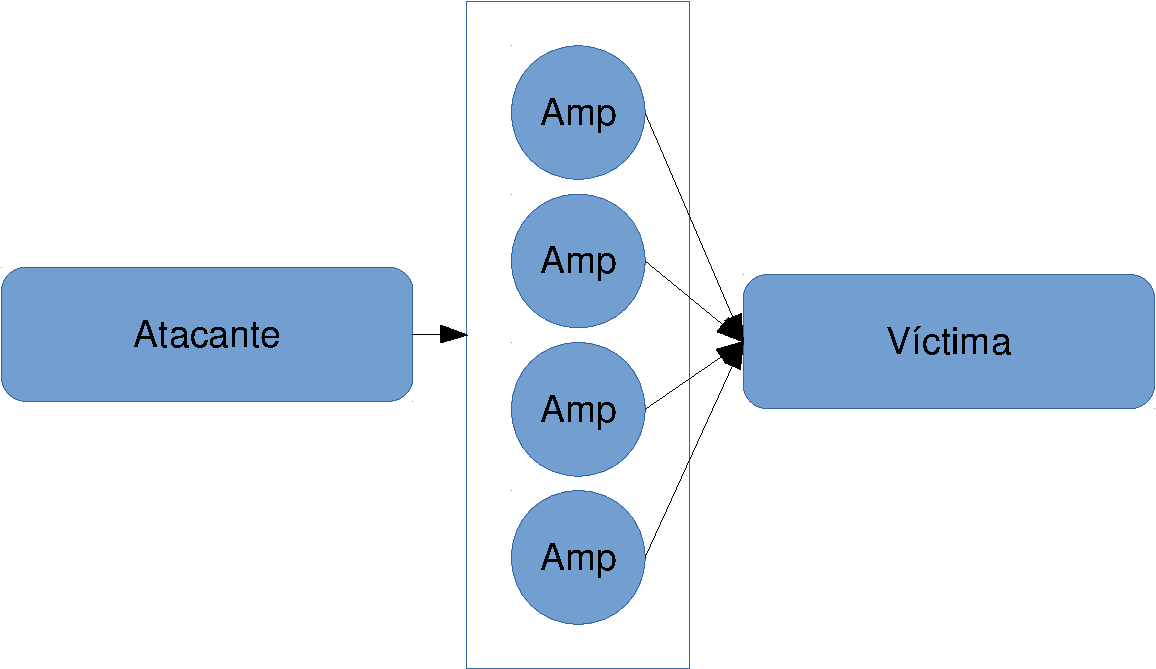
\includegraphics[width=.8\textwidth]{CapituloDDoS/Figuras/Amplificacion}
\caption{Ataque por amplificación}
\LABFIG{amplificacion} %Esto es una forma propia de los autores de gestionar las etiquetas y referencias
\end{figure}
%

Normalmente, este tipo de ataques utilizan la dirección de difusión o broadcast \index{Broadcast} \index{Difusión}. La 
dirección de difusión es una dirección especial en las redes en las que todos los nodos recibirán el paquete. Si ese 
paquete es una petición que requiere una respuesta, y tiene como dirección origen la dirección IP de la víctima (IP 
spoofing\index{IP Spoofing}), todos los nodos de la red responderán el mensaje, saturando la máquina objetivo.

Un ejemplo sencillo de este tipo de ataque es el denominado Ataque \emph{Smurf} \index{Smurf}, que utiliza un 
simple ICMP\index{ICMP} PING\index{ICMP}\index{PING}. Si a todos los nodos de la red les llega una petición de PING 
proveniente de la dirección de la víctima, la víctima se encontrará con tantas respuestas como nodos configurados para 
responder tenga la red. Dichas respuestas tendrán que ser, al menos, procesadas por el sistema operativo de la máquina 
objetivo, que terminará saturando. Por otro lado, el contenido de la respuesta será una copia del contenido de la 
petición, por lo que es sencillo multiplicar (amplificar) el ancho de banda consumido por la víctima emitiendo un 
paquete grande.

Una variante del anterior es el ataque \emph{Fraggle}. El protocolo UDP\index{UDP} tiene su propio sistema de PING, en 
el puerto 7. Además, tiene un sistema de generación de cadenas aleatorias en el puerto 19, el cual envía cadenas de 
texto aleatorias de longitud aleatoria (pero reducida) cualquiera que las pida. De nuevo, la mecánica del ataque es 
falsear la dirección de origen para que estos servicios respondan a la víctima, saturando así la capacidad de sus 
recursos.

\paragraph{Ataques reflejados}\mbox{\newline} \index{Ataques reflejados}

\noindent Para este apartado, un reflector es un nodo que responde a un paquete con otro paquete destinado a la 
dirección origen del primer paquete. Así, podríamos englobar en este apartado, por ejemplo, servidores DNS\index{DNS}. 
Ver \FIG{reflexion}.

\begin{figure}[htbp]
\centering
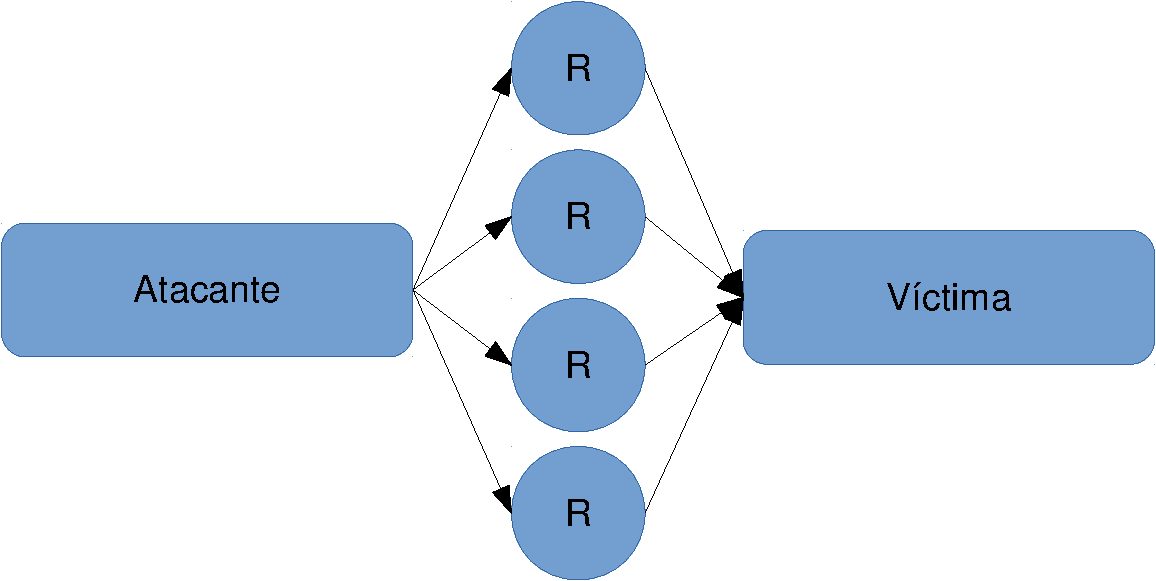
\includegraphics[width=.8\textwidth]{CapituloDDoS/Figuras/Reflexion}
\caption{Ataque por reflexión}
\LABFIG{reflexion} %Esto es una forma propia de los autores de gestionar las etiquetas y referencias
\end{figure}
%

El atacante, entonces, crea una lista de IP reflectoras, y envía para el ataque una petición a cada una de las 
direccionas, con dirección origen la de la vícima. De esta forma, localizar y detener el ataque se vuelve mucho más 
difícil, ya que, siguiendo el ejemplo, cada servidor DNS tiene un dirección IP que no tiene nada que ver con el resto.

Sin embargo, nada impide, en principio, combinar este ataque con el tipo amplificación (por ejemplo, si se 
disponen de muchos DNS en la misma subred). Por otra parte, es posible hacer una petición recursiva a un servidor DNS, 
de forma que en la respuesta viaja el resultado de cada servidor DNS. Esto es, con una pequeña petición (cabecera UDP, 
DNS y nombre de dominio pedido) obtenemos una respuesta mucho mayor, y ya dirigida a la dirección de la victima. 

Así pues, la diferencia entre este tipo y el anterior es que el atacante necesita de una lista de direcciones de host, 
e ir iterando para conseguir el efecto deseado, mientras que en la otra cada paquete se amplificaba mediante el uso de 
la difusión.

\paragraph{Ataques basados en botnets}\mbox{\newline}

\noindent Un bot o zombi es un equipo infectado y controlado remotamente por un maestro. Éste puede ser usado para 
enviar correo no deseado, distribuir malware, espiar (esnifar\index{Esnifar tráfico}) tráfico o, en nuestro caso de 
estudio, para perpetrar un ataque de denegación de servicio. 

Gracias a la red de zombis, el atacante real es mucho más difícil de localizar, además de servir como una primera etapa 
de amplificación del ataque.

\subsubsection{DoS Semánticos}\LABSSSEC{DDoS semanticos}
Esta segunda forma de ataque no se basa en la fuerza bruta o en la extenuación de recursos, sino en 
provocar que el servidor\footnote{O algún elemento de la infraestructura de la comunicación} entre en un estado 
\emph{ilegal}, de forma que no pueda ofrecer el servicio. No es necesario un atacante (o varios) con mucha fuerza, sino 
que se puede llevar a cabo con muy pocos recursos. Sin embargo, requiere un conocimiento mucho más profundo del 
servidor y canal de comunicación. Eso sí, el ataque es más sutil y, lo más importante, puede ser corregido con una 
adecuada configuración o actualización de componentes.
 
Uno de los principales ataques de este estilo consiste en enviar información concreta que sabemos de antemano que 
provocará una caída o malfuncionamiento en el servidor, es decir, aprovechando un fallo de seguridad. Por ejemplo, hasta 
hace relativamente poco (1997), el famoso \emph{ping de la muerte}\index{Ping de la Muerte} \cite{Bidou} era capaz de 
tumbar un servidor con tan 
sólo un comando: \texttt{ping <objetivo>\ -l 65511}, el cual viene integrado en todos los sistemas operativos. Éste 
aprovechaba que la pila ICMP asumía que el paquete tenía una longitud determinada. Al procesar el paquete, y superarse 
esta longitud, se producía un desbordamiento de buffer que hacía que el servidor colapsase.

Otro ejemplo de ataque de este tipo es el ataque \emph{land\index{Land attack}}. En él, la victima recibe un paquete 
TCP cuya dirección origen y destino es él mismo, por lo que intenta contactar consigo mismo hasta que colapsa. 

El ataque \emph{\index{Teardrop}} también es muy famoso, consistente en enviar mensajes IP fragmentados y malformados a 
la muina objetivo. De esta forma, al intentar des-fragmentarlos, la máquina colapsa.

Las nuevas tecnologías tampoco son inmunes a este tipo de ataque. IPv6, por ejemplo, puede sufrir de \emph{Anuncio de 
vecino envenenado\index{Neighbour Advertisement Spoofing Attack}}. En él, un equipo intermedio se anuncia como poseedor 
de una dirección en el camino del cliente al servidor (o bien, la dirección del propio servidor), y anuncia su 
dirección MAC para que todos los paquetes destinados al servidor le lleguen a él. Esto es, es la versión IPv6 del ARP 
spoofing.

\subsection{Objetivo del ataque}
Si queremos ser capaces de defendernos ante un ataque DDoS, es necesario conocer a qué objetivos van destinados. De esa 
forma, podremos centrarnos en defender los activos vulnerables de una forma eficiente.

Podemos clasificar los ataques según el nivel de la capa OSI que atacan en ataques a los routers, a la red, al SSOO o a 
la propia aplicación. Obviamente, un ataque a un nivel inferior afectará a todos los niveles superiores.

\subsubsection{Ataque a dirigido a redes}
La red es el componente más básicos de los ataques DDoS. Si el cliente es incapaz de conectar con la red del servicio, 
es imposible que éste pueda ser ofrecido. Por su parte, si la red del servicio está saturada, ningún cliente será capaz 
de acceder a la misma.

Para agravar las cosas, las aplicaciones confían cada vez más en servicios dependientes de la red. Ejemplo de ello es 
la proliferación de servicios web\index{Servicio web} (aquellos que usan el protocolo \acrshort{HTTP} para su 
funcionamiento), o los servicios en la nube\index{Servicio en la nube} (esto es, aquellos en los que el almacenamiento 
y procesado de datos se realiza en ordenadores remotos, a los que se accede por Internet). 

No solo las redes corporativas exponen sus servicios a Internet. Poco a poco, sistemas críticos, tales como plantas 
generadoras de energía o de procesado de agua, están dentro de una red que, a su vez, en unos pocos saltos están 
conectadas a Internet. De esta forma, estos servicios podrían ser víctimas de un ataque DDoS. Es posible, incluso, que 
el lanzar un ataque hacia otro servicio en esta red intermedia afecte a dicho servicio crítico \cite{Raghavan}.

Así pues, un ataque de denegación de servicio que afectase a dicha infraestructura crítica podría tener repercusiones 
muy serias, tales como dejar sin energía o agua una zona del mapa, y que pocos sistemas escapan actualmente de la 
posibilidad de un ataque DDoS: En el momento que lo conectas a Internet, estás expuesto a ello.

Uno de los protocolos más usados para el transporte de información es \gls{TCP}, por lo que un gran porcentaje de 
ataques van dirigidos contra esta tecnología.

\paragraph{Reseteo de conexiones}\mbox{\newline}

Un ataque muy simple consiste en, una vez que el atacante conoce una conexión existente, resetear dicha conexión. Una 
conexión en \gls{TCP} está identificada por una dirección origen, una dirección destino, un puerto origen y un puerto 
destino. Existe un bit RST\index{TCP RST} en la cabecera \gls{TCP} que permite resetear una conexión inmediatamente. 
Esto es usado, por ejemplo, si uno de los dos extremos detecta un problema en la conexión. Para terminar de empeorar 
las cosas, RST no necesita ACK, por lo que el cliente no llega a saber que la conexión ha terminado

Tras recibir el servidor el RST, el cliente continúa enviando paquetes, y se encontrará con un socket cerrado. El 
servidor enviará otro RST, y será imposible mantener la conexión durante un largo periodo de tiempo. 

Si el atacante ha conseguido localizar una conexión, y es capaz de enviar un paquete TCP con dicho bit activo, el 
receptor de dicho paquete no aceptará más paquetes de esa conexión, y, por tanto, se habrá conseguido que la conexión 
quede invalidada. Podemos ver una descripción gráfica de este ataque en la \FIG{RST attack}.

\begin{figure}[htbp]
\centering
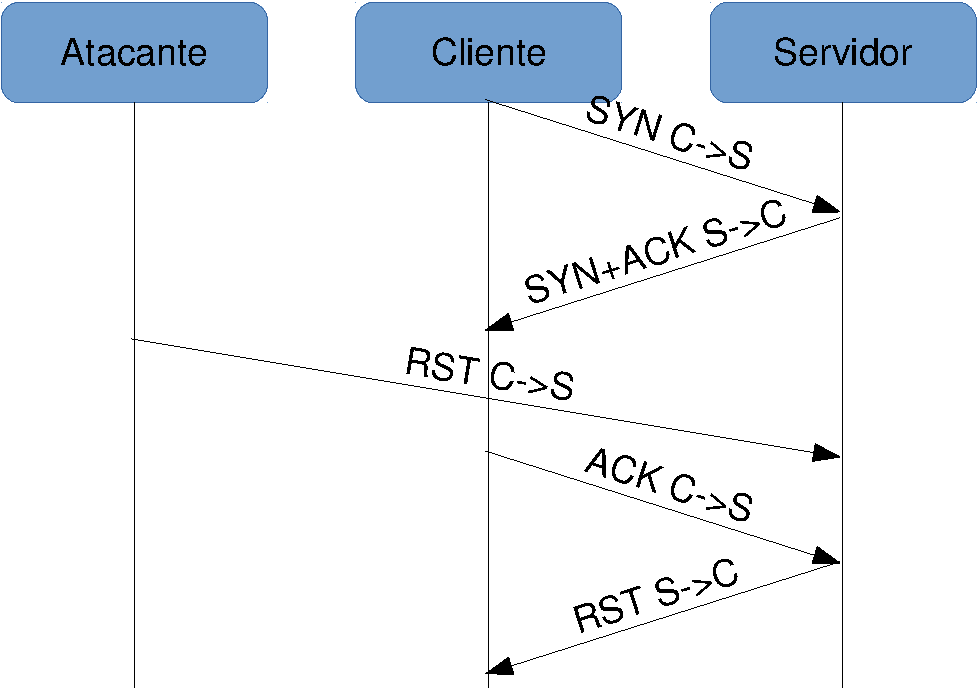
\includegraphics[width=.8\textwidth]{CapituloDDoS/Figuras/RST_attack}
\caption{Ataque RST}
\LABFIG{RST attack} 
\end{figure}
%

\paragraph{Asentimientos optimistas}\mbox{\newline}

Otra característica comúnmente explotada de las conexiones \gls{TCP} es su control de congestión\index{Control de 
congestión TCP}. Para calcular la saturación del enlace, un extremo considera como paquete perdido (y, por tanto, el 
enlace está saturado) aquel paquete que tarda más de $T$ segundos en recibir el ACK. Al iniciar la conexión TCP, el 
algoritmo de arranque lento\index{TCP slow start} incrementará el número de paquetes enviados de una forma exponencial.

Si el atacante envía ACK optimistas, esto es, ACK de un paquete que realmente no ha recibido aún, el atacante enviará 
cada vez más y más paquetes salientes, hasta saturar su conexión. Teniendo en cuenta que un TCP ACK sólo ocupa 54 
bytes, el efecto amplificador de este tipo de ataque es bastante importante. Algunos estudios hablan de que, con una 
conexión de 56kbps, es posible generar en el lado del atacante unos 8.9mbps \cite{sherwood}.

Podemos ver un ejemplo de este tipo de ataques en la \FIG{optim ACK attack}.

\begin{figure}[htbp]
\centering
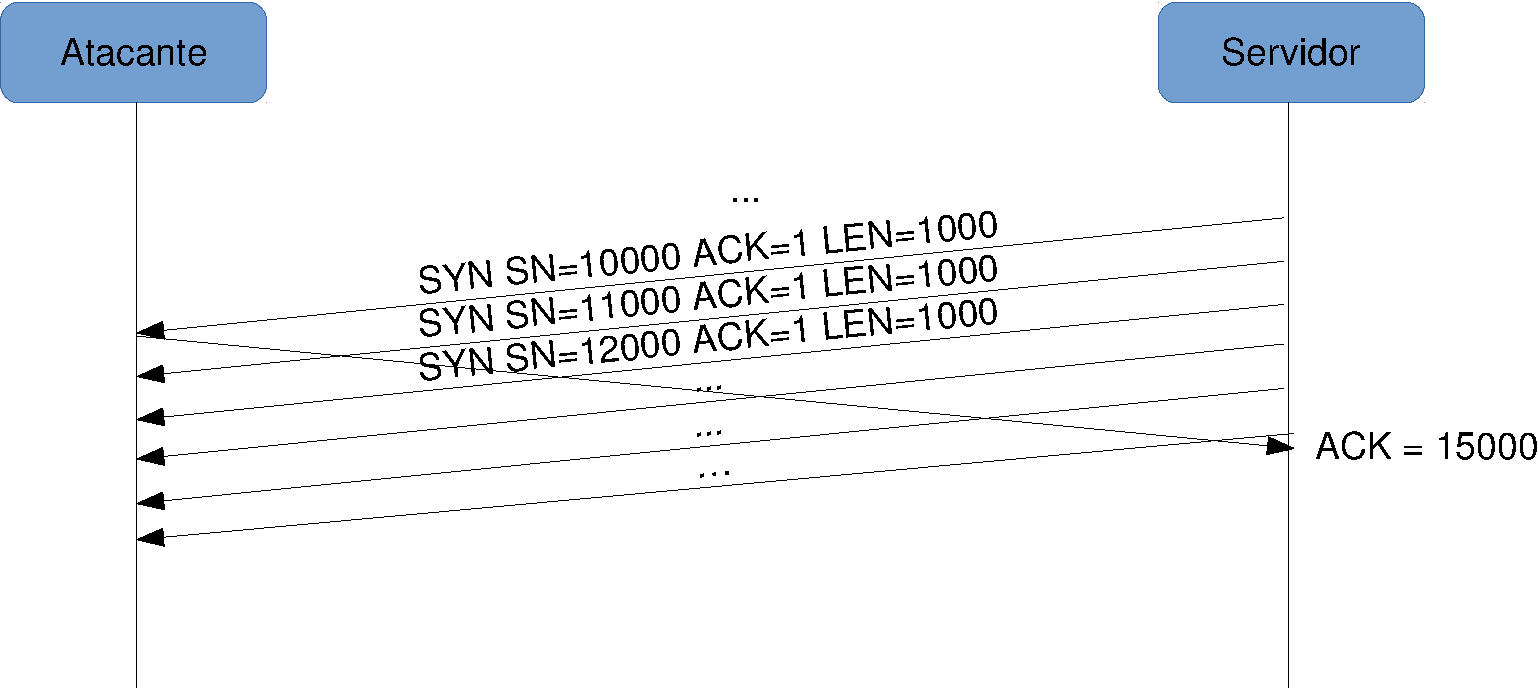
\includegraphics[width=\textwidth]{CapituloDDoS/Figuras/optim_ACK_attack}
\caption{Ataque por ACK optimista}
\LABFIG{optim ACK attack} 
\end{figure}
%

\paragraph{Temporizador de retransmisión}\mbox{\newline}

Cuando un paquete se pierde en una conexión \gls{TCP}, el protocolo dice que es necesario reenviarlo. Como ya hemos 
explicado, un paquete perdido es aquel que no recibe el ACK correspondiente.

El atacante podría saturar los dispositivos de comunicación si envía una gran inundación de paquetes a los mismos. Sin 
embargo, esto sería fácilmente detectable por dispositivos que monitorizan la red.

En su lugar, el atacante enviará una ráfaga de corta duración pero de mucha intensidad, lo suficiente para saturar los 
dispositivos y hacer perder paquetes. En este caso, \gls{TCP} alcanzará el estado de \emph{timeout} en todas las 
comunicaciones, y necesitará comenzar a retransmitir los paquetes por donde iba la conexión.

Siguiendo el procedimiento de \gls{TCP}, se debe comenzar a retransmitir los paquetes en ráfagas, empezando por un 
paquete por ráfaga e ir aumentando progresivamente. En poco tiempo, se debería volver a alcanzar un buen rutmo para la 
conexión.

Sin embargo, si el atacante, al acabar el temporizador de retransmisión, vuelve a lanzar otro ataque intensivo pero de 
corta intensidad y vuelve a saturar los elementos de comunicación, las conexiones no serán capaces de recuperarse.

Así pues, el atacante ha aprovechado el propio tiempo de retransmisión \gls{TCP} para dejar incomunicado el servidor, y 
de esa forma amplificar su ataque: Con ráfagas cortas, es capaz de producir el mismo efecto que si saturase el canal 
continuamente. Menos ancho de banda consumido, y menos probabilidades de detección.

En la \FIG{RTO attack} podemos ver el perfil que tendría el tráfico atacante para bloquear la comunicación. En ella, 
$I_p$ es la intensidad del pico del ataque, $T_p$ es la duración del pico atacante, y $T_{timeout}$ es el temporizador 
de retransmisión que tiene \gls{TCP}.

\begin{figure}[htbp]
\centering
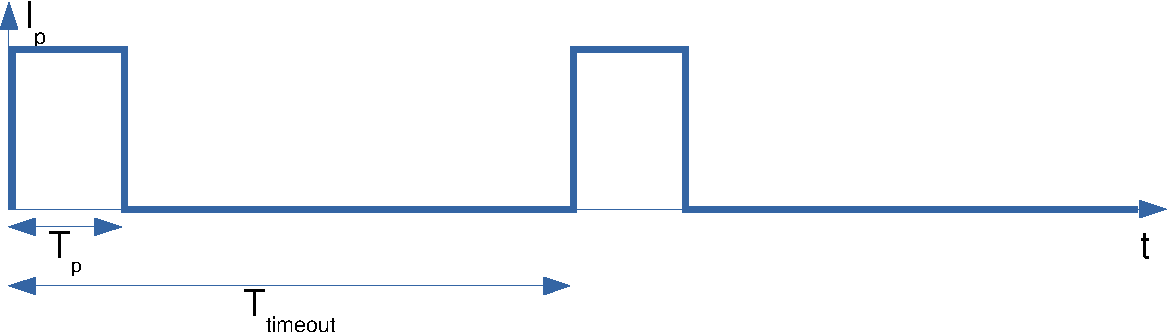
\includegraphics[width=\textwidth]{CapituloDDoS/Figuras/RTO_attack}
\caption{Ataque por retransmisión TCP}
\LABFIG{RTO attack} 
\end{figure}
%

\subsubsection{Ataque a Sistemas Operativos}\LABSSSEC{Ataques a SSOO}

El encargado de transportar correctamente los paquetes desde la red hasta la aplicación. Si el atacante es capaz de 
hacer que este intermediario no sea capaz de llevar los paquetes desde o hacia la aplicación, habrá logrado llevar a 
cabo un ataque \gls{DoS}.

En este tipo de ataque se busca explotar una vulnerabilidad en el modo que el \gls{SO} gestiona los paquetes. Por 
ejemplo, si a la hora de recibir un paquete, el \gls{SO} lo escribe en memoria sin comprobar los límites de la memoria 
reservada para ello, el atacante podría enviar un paquete lo suficientemente largo como para provocar un \emph{buffer 
overflow}\index{Buffer Overflow}, esto es, se escribirá en una zona de memoria indebida, provocando que el sistema 
colapse. Esta técnica es la empleada por el llamado \emph{ping de la muerte}\index{Ping de la Muerte}, ya explicado en 
el \SSSEC{DDoS semanticos}.

Otro ataque, también dirigido a saturar el \gls{SO}, sería un SYN flood (inundación SYN). Esta vez, con la inundación, 
no provocamos saturar la red, sino la capacidad de conexiones simultaneas que aguante el sistema.

\subsubsection{Ataques dirigidos a aplicaciones (Ataques capa 7)}

Muchas aplicaciones están desarrollando sus aplicaciones sobre una arquitectura tipo servicio web, esto es, programas 
distribuídos que funcionan mediante el paso de mensajes sobre el protocolo HTTP. Para que este servicio funcione, si 
está expuesto a internet, es necesario que el cortafuegos permita el tráfico hacia esa aplicación. Por tanto, el 
atacante es capaz también de alcanzar dicho servicio, aunque quizás no pueda usarlo por necesitar, por ejemplo, unas 
credenciales válidas.

Al igual que los servicios web, la aplicación distribuída puede estar confiando en cualquier otro tipo de tecnología 
subyacente. Mientras que esta se encuentre en espacio de usuario, se considerará un ataque de capa 7.

Los métodos para realizar este ataque son muy parecidos a los de la \SSSEC{Ataques a SSOO}. Por la parte semántica, se 
puede intentar enviar información corrupta que haga al servidor entrar en un estado incorrecto, que no pueda continuar 
sirviendo. Por otra parte, tenemos los ataques por inundación, que buscarían saturar la capacidad del servidor, y que 
a la máquina le sea imposible seguir respondiendo peticiones.


\section{Técnicas de detección y mitigacinó de un ataque DDoS}
\subsection{Ataques por inundación}
La principal señal que indica que un servicio está sufriendo un ataque por inundación es que reciben una cantidad de 
tráfico anormalmente grande. Sin embargo, para una detección correcta deberíamos definir qué supone \emph{anormal}. 

A lo largo de este trabajo intentaremos definir un sistema de detección de anomalías (CUSUM, \CHAP{TODO}), y qué 
parámetros debemos usar para buscar un compromiso entre velocidad de detección y no aparición de falsos positivos.

%TODO aún falta el tunning: Dificuktad de definir normal y anormal. Problemas de refinamiento.

Para mitigar el ataque, no basta con cortar el acceso al servicio, ya que entonces el \gls{DDoS} habría triunfado. Es 
necesario discernir entre las direcciones IP maliciosas o atacantes, y cortar el tráfico sólo a ellas, permitiendo que 
las direcciones benignas sigan navegando como hasta ahora.

\subsection{Ataques semánticos}
Para la detección de ataque ssemánticos, el método más usado es la detección de patrones. Esto es, analizar el paquete 
en busca de características del mismo que detecten que estamos ante un paquete, al menos sospechoso. Al patrón que 
siguen esos paquetes maliciosos y que, por tanto lo hace detectable, se le denomina \emph{firma}\index{Firma}.

Por ejemplo, en el caso del \emph{ping de la muerte}, un sistema intermedio podría analizar todos los paquetes que van 
hacia el servidor y, en caso de ser de un tamaño superior o igual a $2^16=65536$, bloquar el paso de dicho paquete.

Comparativamente hablando, tienen la desventaja de necesitar la constante actualización de la base de datos de firmas, 
y la posibilidad de que esta base de datos crezca, haciendose más inmanejable. Su refinamiento consiste en la selección 
de reglas adecuadas a los activos protegidos, esto es: Si no tengo un servidor web, no necesito estar analizando 
paquetes contra firmas que comprometen servidores web, es un gaso inútil.

Este es el sistema de detección usado por IPS tales como snort \cite{snort} o suricata \cite{suricata}. A lo largo de 
este trabajo no pretenderemos abarcar este tipo de soluciones.

\section{Resumen}%%%%%%%%%%%%%%%%%%%%%%%%%%%%%%%%%%%%%%%

\begin{Resumen}[Resumen del capítulo]
\subsection*{Definición}
Acción(es) que impiden que un sistema de información funcione normalmente.

\subsection*{Taxonomía}
\begin{align*}
 \begin{cases}
   \text{Por inundación.}
   \begin{cases}
     \text{Coordinados por seres humanos / manuales.}\\
     \qquad\text{\emph{Ningún elemento automático}}\\
     \text{Amplificados.}\\
     \qquad{\text{\emph{El atacante sólo envía N y el ataque se amplifica}}}\\
     \qquad{\text{\emph{Ejemplo: ping a direcciones broadcast}}}\\
     \text{Reflejados.}\\
     \qquad{\text{\emph{El atacante tiene una lista de IP que pueden reflejar su ataque}}}\\
     \qquad{\text{\emph{Ejemplo: Peticiones DNS con dirección origen de la víctima}}}\\
     \text{Botnets o redes Zombi.}\\
     \qquad{\text{\emph{Efecto amplificador y ocultador}}}
     \text{Combinación de las anteriores.}
   \end{cases}\\
   \text{Semántico.}\\
   \qquad{\text{\emph{Se busca explotar fallos}}}
 \end{cases}
\end{align*}

\subsection*{Objetivo del ataque}
\begin{align*}
 \begin{cases}
   \text{Dirigido a redes.}\\
   \qquad{\text{\emph{Ejemplos:}}}
   \begin{cases}
     \text{Reseteo de conexiones.} \\
     \text{Asentimientos optimistas.} \\
     \text{temporizador de retransmisión.} \\
   \end{cases}\\
   \text{Ataques a SSOO.} \\
   \text{Ataques de capa 7.}\\
 \end{cases}
\end{align*}

\subsection*{Técnicas de detección y mitigación}
\begin{align*}
 \begin{cases}
   \text{Por inundación.}
   \begin{cases}
     \text{Detección de comportamiento \emph{anómalo} en la red.} \\
     \qquad\rightarrow\text{¿Definición de anómalo?} \\
     \text{Bloqueo de direcciones con comportamientos anómalos}\\
     \qquad\rightarrow\text{Posibilidad de falsos negativos y falsos positivos}\\
     \text{Tuneado consistente en definir \emph{normal}}
   \end{cases}\\
   \text{Semánticos}
   \begin{cases}
     \text{Detección de patrones (firmas) en el tráfico.} \\
     \qquad\rightarrow\text{Necesidad de actualización} \\
     \text{Bloqueo de paquetes que cumplan dichos patrones}\\
     \qquad\rightarrow\text{Posibilidad de falsos negativos y falsos positivos} \\
     \text{Tuneado consiste en seleccionar reglas en base a los activos a proteger}
   \end{cases}\\
 \end{cases}
\end{align*}

\end{Resumen}


%
% !TEX root =../LibroTipoETSI.tex
\chapter{El algoritmo CUSUM}\LABCHAP{Algoritmo CUSUM}
\pagestyle{esitscCD}
\epigraph{ El objetivo de un sistema de control es el de establecer un sistema de observación permanente e 
inteligente, que detecte la aparición de variabilidad sobre la norma e identifique su origen. }{Ismael Sánchez, Dpto de 
Estadística y Econometría, Universidad Carlos III}

%\lettrine[lraise=0.7, lines=1, loversize=-0.25]{E}{l} 
\lettrine[lraise=-0.1, lines=2, loversize=0.25]{E}n el \CHAP{Denegacion de Servicio} se dio la clave para detectar y 
protegerse ante un ataque de denegación de servicio por inundación: Se debe monitorizar el tráfico, extraer sus 
parámetros típicos, y comprobar contínuamente si el tráfico actual entra dentro de lo \emph{normal}. Es lo que 
normalmente se denomina \emph{control de procesos}.

A lo largo de este capítulo, daremos una definición formal a lo que se denomina \gls{CdP}, y comprobaremos tras 
estudiarlo  que nos es útil para la monitorización de tráfico y su caracterización. Tras ello, pasaremos a ver el 
algoritmo \gls{CUSUM}, un \gls{SCP} con memoria, esto es, es capaz de controlar un proceso no sólo por el estado actual 
sino que también tiene en cuenta los estados anteriores por los que ha pasado.

Por último, explicaremos el uso del algoritmo \gls{CUSUM} que hemos hecho en este trabajo: Qué parámetros del tráfico 
hemos escogido revisar para detectar ataques, por qué esos y cómo los monitorizamos, y esbozaremos el protocolo de 
actuación seguido cuando alguno de estos parámetros se escapa de control.

\section{Control de procesos}\index{Control de Procesos}

Mediante el \gls{CdP}\index{Control de Procesos} se intenta diferenciar entre las causas \emph{comunes} y las causas 
\emph{especiales} de la variablidad. Esto es, diferenciar entre las pautas \emph{normales} de un proceso, debidas a su 
propia operativa, y las desviaciones esporádicas sobre esa pauta, que provocan que el proceso \emph{salga del control}.

Su objetivo es el de establecer un sistema de observación permanente e inteligente, que detecte la aparición de 
variabilidad sobre la norma e identifique su origen, de forma que sea posible evitar su reaparición 
\cite{Control_de_procesos}.

Así pues, un \gls{SCP}\index{Sistema de Control de Procesos} permitiría medir las características \emph{normales} del 
tráfico, y detectar de una forma temprana si estamos ante un tráfico normal o, por el contrario, estamos bajo un 
tráfico anómalo y, por tanto, bajo un posible ataque.

\section{Algoritmo CUSUM}\index{CUSUM}
Dadas unas muestras de un proceso $x_1$, $x_2$, ..., podríamos dibujar un gráfico de la forma $f(x_1)$, $f(x_2)$, ... 
cuyas características nos dijese si el proceso se encuentra o no bajo control\index{Proceso Bajo Control}\index{Proceso 
Fuera de Control}. Por ejemplo, si $f(x_j) > H$, decimos que el proceso se ha salido de control en la iteración $j$.

El algoritmo \gls{CUSUM} es un sistema de control con memoria\index{Sistema de Control de Procesos con Memoria}, esto 
es, dadas las muestras $x_1,x_2,..$, el gráfico de control estudia la evolución de 
$f(x_1),f(x_1,x_2),f(x_1,x_2,x_3),f(x_1,x_2,x_3,...)$. Como la información se va acumulando, si se produce un pequeño 
desajuste durante un periodo de tiempo, este acaba detectándose 
\cite{CUSUM_Carlos_III}.

Ante una Variable de Interés $x_i$, que sigue una distribución normal $x_i \sim\mathcal{N}\left(\mu_0,\sigma^2\right)$, 
construimos el estadístico $C_i$ que acumula la información:
\begin{align}
 C_1 &= (x_1 - \mu_0) \nonumber\\
 C_2 &= (x_1 - \mu_0) + (x_1 - \mu_0) = C_1 + (x_2-\mu_0) \nonumber\\
 &\vdots& \nonumber\\
 C_i &= C_{i-1} + (x_i-\mu_0) \LABEQ{CUSUM}
\end{align}

Esto es, $C_i$ acumula la desviación de $x_j \forall j\in(0,i-1)$ sobre su media. Si el proceso está bajo control, las 
desviaciones deberían acumularse, y, por tanto, contrarrestarse. $C_i$ debería evolucionar sobre una horizontal de 
nivel $0$. Esto es, para un proceso bajo control:
\begin{align}
 \mathbb{E}(C_i) &= \mathbb{E}\left[\left(x_1 - \mu_0\right) + \left(x_2-\mu_0\right)+\hdots
                                                                             +\left(x_i-\mu_0\right)\right] \nonumber\\
                 &= \mathbb{E}\left[\sum_{j=1}^i\left(x_j-\mu_0\right)\right]                               \nonumber\\
                 &= \sum_{j=1}^i\mathbb{E}\left(x_j-\mu_0\right)                                            \nonumber\\
                 &= \sum_{j=1}^i\mathbb{E}\left(x_j\right) - \sum_{j=1}^i\mu_0 = i\mu_0 - i\mu_0 = 0
 \end{align}

\begin{figure}[htbp]
\centering
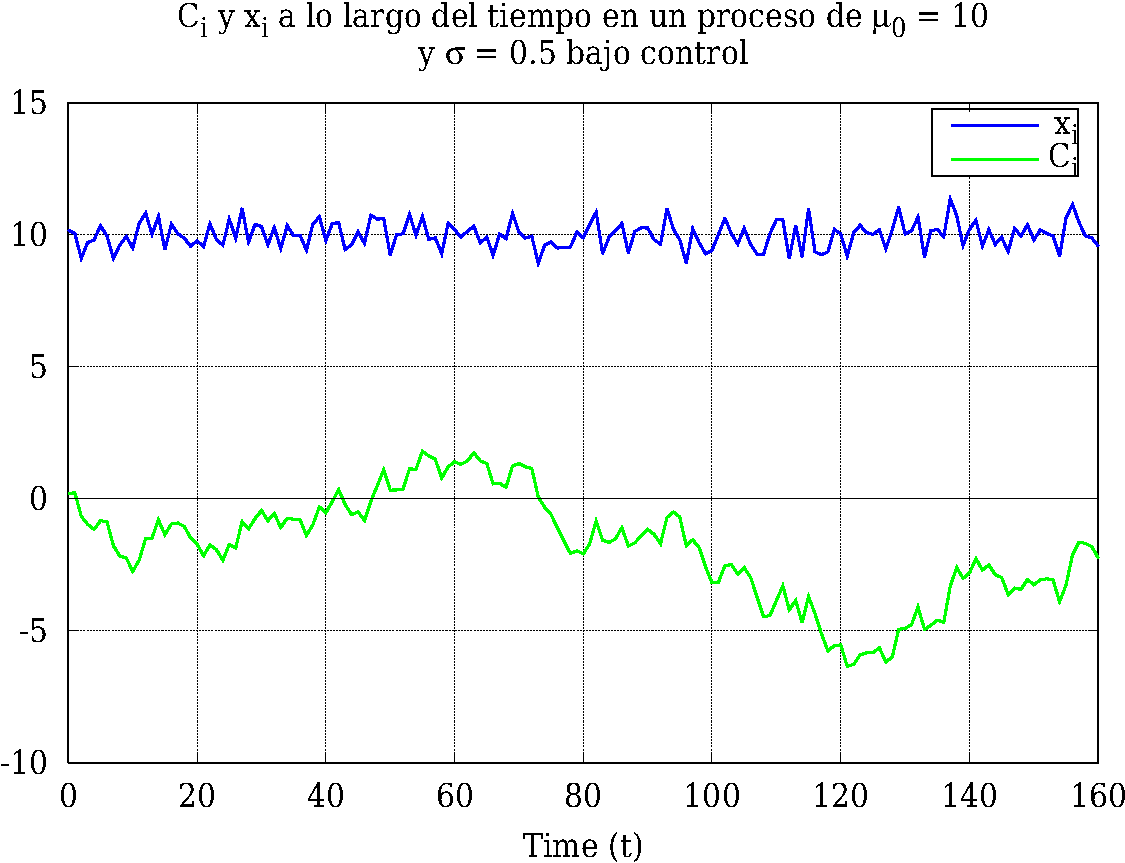
\includegraphics[width=0.9\textwidth]{CapituloCusum/Figuras/ejemploCusumControlado_crop}
\caption{Algoritmo CUSUM aplicado sobre un proceso controlado}
\LABFIG{cusum_controlado} 
\end{figure}
%

\begin{lstlisting}[language=Matlab,caption={Algoritmo CUSUM en procesos bajo control}, breaklines=true, 
label=code:cusum_controlado,numbers=left,float=hbtp]
clear all
close all

N     = 161; % Número de muestras
sigma = 0.5; 
mu    = 10;

x = [0:N-1];
y = mu + sigma*randn(1,N);
z = zeros(1,N);

z(1) = y(1)-mu;
for i=2:N
    z(i) = z(i-1) + (y(i) - mu);
end

plot(x,y,'color','blue','LineWidth',4)
plot(x,z,'color','green','LineWidth',4);
plot([0,N-1],[0,0],'color','black')
axis([0,N-1])
\end{lstlisting}

Para hacernos una idea visual, generamos una gráfica con el código octave \autoref{code:cusum_controlado}, y vemos su 
resultado en la \FIG{cusum_controlado}.

Si el procedimiento está bajo control, vemos cómo $C_i$ oscila en torno al 0, con mayor o menor desviación.

Por su parte, si desajustamos el proceso, y su media comienza a valer $\mathbb{E}(x) = \mu_0 + k$:

\begin{align}
 \mathbb{E}(C_i) &= \mathbb{E}\left[\left(x_1 - \mu_0\right) + \left(x_2-\mu_0\right)+\hdots
                                                                             +\left(x_i-\mu_0\right)\right] \nonumber\\
                 &= \mathbb{E}\left[\sum_{j=1}^i\left(x_j-\mu_0\right)\right]                               \nonumber\\
                 &= \sum_{j=1}^i\mathbb{E}\left(x_j-\mu_0\right)                                            \nonumber\\
                 &= \sum_{j=1}^i\mathbb{E}\left(x_j\right) - \sum_{j=1}^i\mu_0 = i\left(\mu_0 + k\right) - i\mu_0 = ik
                                                                                             \LABEQ{cusum_descontrol}
\end{align}

Se extrae de la \EQ{cusum_descontrol} que $C_i$ seguirá una recta $C_i=ik$ de pendiente $k$. Volvemos a generar una 
gráfica \FIG{cusum_descontrolado} con el código \autoref{code:cusum_descontrolado}.

\begin{figure}[htbp]
\centering
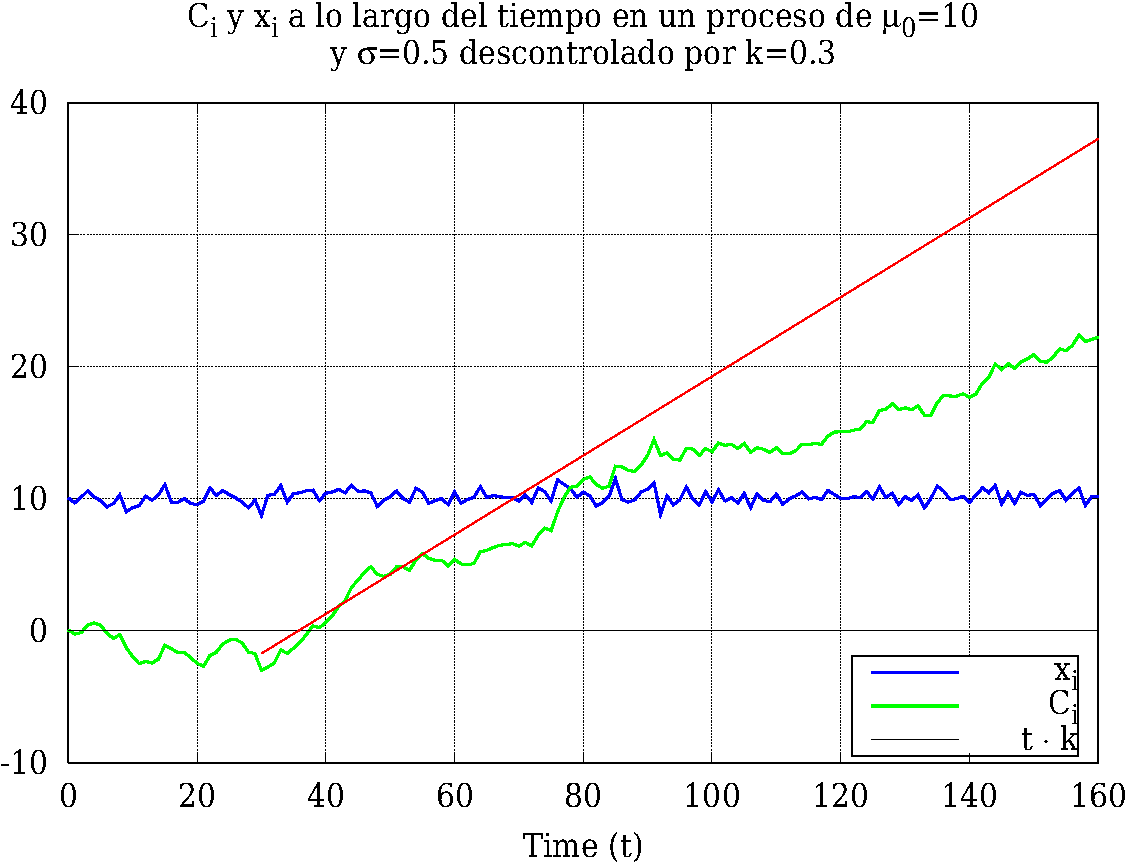
\includegraphics[width=0.9\textwidth]{CapituloCusum/Figuras/cusumDescontrolado-crop}
\caption{Algoritmo CUSUM aplicado sobre un proceso perturbado}
\LABFIG{cusum_descontrolado} 
\end{figure}
%

\begin{lstlisting}[language=Matlab,caption={Algoritmo CUSUM en procesos perturbados}, breaklines=true, 
label=code:cusum_descontrolado,numbers=left,float=htbp]
clear all
close all

N     = 161; % Número de muestras
M     = 30;  % Instante en el que se aplica el descontrol
sigma = 0.5; 
mu    = 10;

x = [0:N-1];
y = mu + sigma*[randn(1,M) k+randn(1,N-M)];
z = zeros(1,N);

z(1) = y(1)-mu;
for i=2:N
    z(i) = z(i-1) + (y(i) - mu);
end

plot(x,y,'color','blue','LineWidth',4)
plot(x,z,'color','green','LineWidth',4);
plot([M,N],[z(M),z(M)+k*(N-M)],'color','red'
plot([0,N-1],[0,0],'color','black')
\end{lstlisting}

Se observa en las figuras que, debido a la extrema sensibilidad que presenta este algoritmo es fácil que el mismo no 
siga la recta predicha en pocas iteraciones. Por eso, el \gls{CUSUM} algorítmico  sólo tendrá en cuenta desviaciones 
que superen un cierto umbral de sensibilidad $K$\index{Umbral de sensibilidad}.

\begin{align}
 C_i^+ &= \max \left[0,\left\{C_{i-1}^+\left(x_i-\mu_0\right)\right\}-K\right] \\
 C_i^- &= \max \left[0,\left\{C_{i-1}^-\left(x_i-\mu_0\right)\right\}-K\right]
\end{align}

Donde $C_i^+$ detecta las desviaciones positivas y $C_i^-$ las negativas.

Es decisión del analista determinar el umbral $K$. Si se quiere detectar un desajuste de $\delta\mu_0=\delta\sigma$,es 
decir, $\mu_1 = \mu_0 + \delta\sigma$ se suele tomar:

\begin{align}
 K = \frac{\delta}{2}\sigma = \frac{\left|\mu_0-\mu_1\right|}{2}
\end{align}

Volvemos a pintar ambas gráficas con el nuevo umbral de sensibilidad en \FIG{cusum_controlado_umbral_sensibilidad} y 
\FIG{cusum_descontrolado_umbral_sensibilidad}, usando \autoref{code:cusum_controlado_umbral} y 
\autoref{code:cusum_descontrolado_umbral}

\begin{figure}[htbp]
\centering
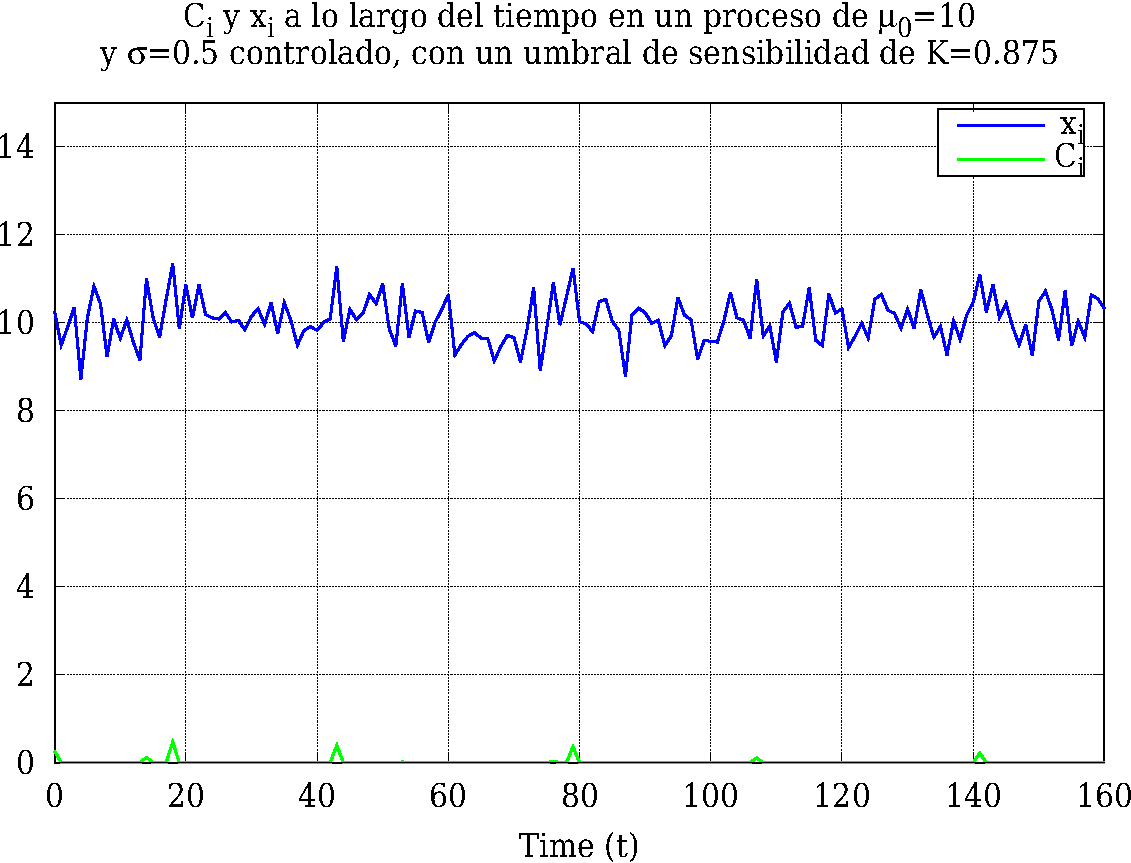
\includegraphics[width=0.9\textwidth]{CapituloCusum/Figuras/cusumControladoUmbral-crop}
\caption{Algoritmo CUSUM aplicado sobre un proceso controlado usando un umbral de sensibilidad}
\LABFIG{cusum_controlado_umbral_sensibilidad} 
\end{figure}
%

\begin{figure}[htbp]
\centering
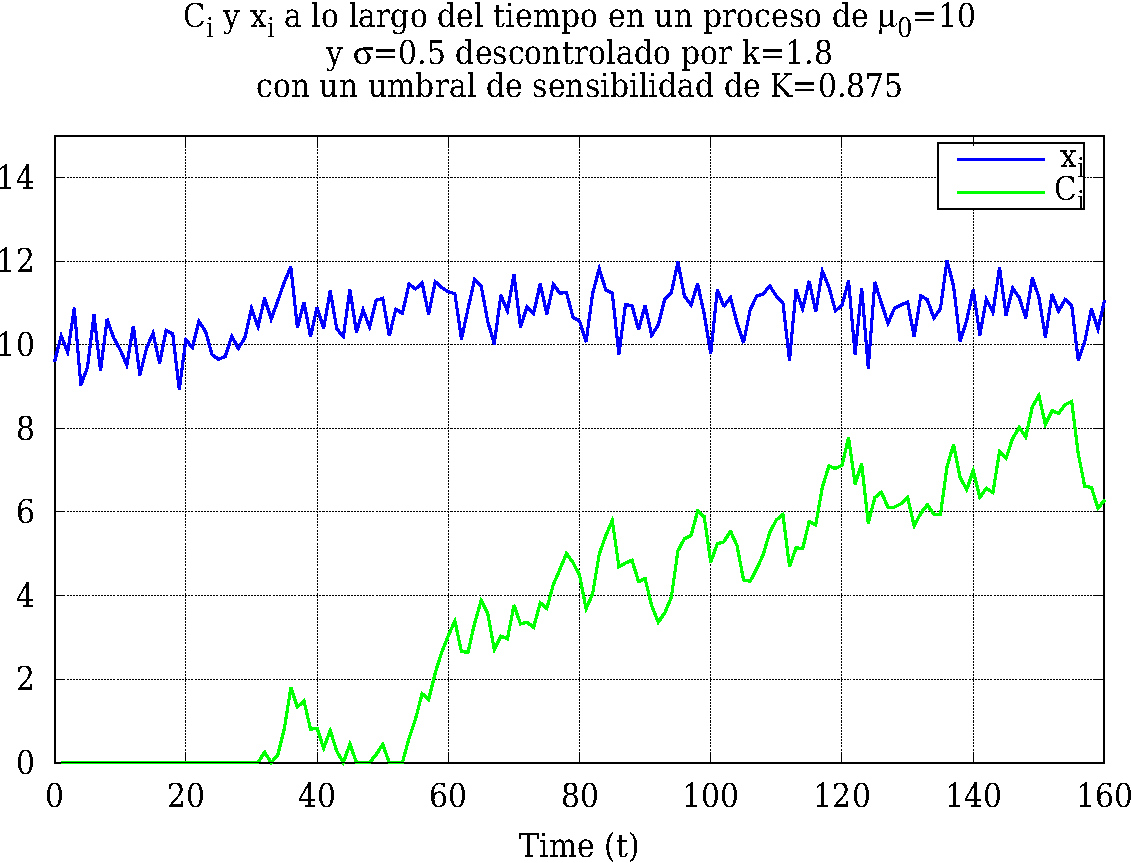
\includegraphics[width=0.9\textwidth]{CapituloCusum/Figuras/cusumDescontroladoUmbral-crop}
\caption{Algoritmo CUSUM aplicado sobre un proceso descontrolado usando un umbral de sensibilidad}
\LABFIG{cusum_descontrolado_umbral_sensibilidad} 
\end{figure}
%

\begin{lstlisting}[language=Matlab,caption={Algoritmo CUSUM en procesos bajo control con umbral de sensibilidad}, 
breaklines=true, label=code:cusum_controlado_umbral,numbers=left,float=htbp]
clear all
close all

N     = 161;        % Número de muestras
M     = 30;         % Instante en el que se aplica el descontrol
sigma = 0.5; 
mu    = 10;
k     = 0;          % Desviación sobre la media
K     = 1.75*sigma; % Umbral de sensibilidad

x = [0:N-1];
y = mu + sigma*[randn(1,M) k+randn(1,N-M)];
z = zeros(1,N);

z(1) = y(1)-mu;
for i=2:N
  z(i) = max(z(i-1) + (y(i) - mu) - K,0);
end

plot(x,y,'color','blue','LineWidth',4)
plot(x,z,'color','green','LineWidth',4);
plot([M,N],[z(M),z(M)+k*(N-M)],'color','red'
plot([0,N-1],[0,0],'color','black')
\end{lstlisting}

\begin{lstlisting}[language=Matlab,caption={Algoritmo CUSUM en procesos perturbados con umbral de sensibilidad}, 
breaklines=true, label=code:cusum_descontrolado_umbral,numbers=left,float=htbp]
clear all
close all

N     = 161;        % Número de muestras
M     = 30;         % Instante en el que se aplica el descontrol
sigma = 0.5; 
mu    = 10;
k     = 1.8;        % Desviación sobre la media
K     = 1.75*sigma; % Umbral de sensibilidad

x = [0:N-1];
y = mu + sigma*[randn(1,M) k+randn(1,N-M)];
z = zeros(1,N);

z(1) = y(1)-mu;
for i=2:N
  z(i) = max(z(i-1) + (y(i) - mu) - K,0);
end

plot(x,y,'color','blue','LineWidth',4)
plot(x,z,'color','green','LineWidth',4);
plot([M,N],[z(M),z(M)+k*(N-M)],'color','red'
plot([0,N-1],[0,0],'color','black')
\end{lstlisting}

Por último, restaría estudiar un umbral de control $H$\index{Umbral de Control}, a partir del cual emitiríamos la 
alarma si $C_i^+$ o $C_i^-$ sobrepasase dicho valor. Generalmente, $H=5\sigma$, pero, de nuevo, depende de la 
sensibilidad del algoritmo el escoger un valor u otro.

\section{Algoritmo CUSUM aplicado al control del tráfico}\index{Control del tráfico}
El tráfico de red es muy dificil de modelar, debido a su naturaleza caótica. Para comenzar, existen muchísimas 
características que podríamos tener en cuenta a la hora de controlar: número de paquetes, paquetes TCP con un bit 
concreto activado\footnote{Esto suma 6 nuevas características}, número de paquetes dirigidos a la misma IP, o desde la 
misma, número de paquetes dirigidos a un servicio particular\footnote{$2^{16}=65536$ posibilidades para TCP y otras 
tantas para UDP}, etc. 

Por otro lado, sean cuales sean los parámetros escogidos, ¿cuáles son sus valores normales? El valor de tráfico normal 
para la página de Slashdot es un ataque de denegación de servicio brutal para las páginas de las noticias que 
enlazan\footnote{Este ataque fue explicado en el \SSSEC{DoS por inundacion}}. Otro elemplos son los denominados 
\emph{Eventos Flash}\index{Eventos Flash}, en los que se produce un incremento de tráfico legítimo \cite{Raghavan}.

En esta sección, describiremos cómo aplicar el algoritmo CUSUM al modelado y caraterización del tráfico: Qué parámetros 
conviene revisa y por qué se han elegido esos (\SSEC{Parametros de interés}), y por qué son neecsarios y cómo debe 
funcionar el sistema de defensa en el periodo de aprendizaje y defensa, así como las aciones que debe tomar si detecta 
que estamos bajo un posible ataque (\SSEC{Periodo de aprendizaje} y \SSEC{Periodo de defensa}).

\subsection{Parámetros de interés}\LABSSEC{Parametros de interés}
S.V. Raghvan y E.Dawson señalan los siguientes como los parámetros más importantes a la hora de detectar un ataque 
\gls{DoS}:

\begin{itemize}
 \item \gls{OWCD}, Densidad de conexiones de un solo sentido
 \begin{align}
  \text{OWCD} = \frac{\sum\text{Paquetes OWC}}{\sum\text{Paquetes IP}}
 \end{align}

 \item Longitud media de paquetes.
 \begin{align}
  <L>_{\text{flow}} = \frac{\sum\text{Paquetes IP}}{\sum\text{Flujos IP}}
 \end{align}
 
 \item Relación paquetes entrantes y salientes
 \begin{align}
  R_{io} = \frac{\sum\text{Paquetes entrantes}}{\sum\text{Paquetes salientes}}
 \end{align}
 
 \item Porcentaje de paquetes TCP
 \begin{align}
  R_{io} = \frac{\sum\text{Paquetes TCP}}{\sum\text{Paquetes IP}}
 \end{align}
 
 \item Porcentaje de paquetes UDP
 \begin{align}
  R_{io} = \frac{\sum\text{Paquetes UDP}}{\sum\text{Paquetes IP}}
 \end{align}
 
 \item Porcentaje de paquetes ICMP
 \begin{align}
  R_{io} = \frac{\sum\text{Paquetes ICMP}}{\sum\text{Paquetes IP}}
 \end{align}
 
 \item Porcentaje de paquetes LAND, esto es, que tienen la misma dirección IP origen y destino
 \item Tipo de potocolo: \gls{TCP}, \gls{UDP}, \gls{ICMP}... 
\end{itemize}

Para la obtención de dichos parámetros, se monitorizará el tráfico desde y hacia el activo protegido por cada IP 
externa\footnote{Más adelante definiremos el concepto de \gls{IP} externa, en la sección \ref{TODO}. Por ahora, se 
trata de la \gls{IP} que intenta acceder al activo defendido, o a la que el activo defendido está respondiendo.}, 
acumulando los bytes y paquetes por protocolo, bytes y paquetes entrantes y salientes, el conteo de los paquetes LAND, 
los paquetes \gls{TCP} \gls{SYN} y aquellos marcados con los bits \gls{SYN} y \gls{ACK} al mismo tiempo. 

Tras intervalos de tiempo regulares, se extraerá de ese conteo los parámetros enumerados anteriormente, lo que supondrá 
una muestra de cada estadístico por cada IP, más una muestra global.

Según los datos aprendidos a lo largo del tiempo, y los datos que aprendamos en este intervalo de tiempo, el programa 
puede estar en estado \emph{Aprendizaje}, en estado \emph{Defensa} o en estado \emph{Alarma} (ver 
\FIG{diagrama_estados}). En qué consiste cada estado, y las causas de las transiciones se encuentran en las siguiente 
secciones.

\begin{figure}[htbp]
\centering
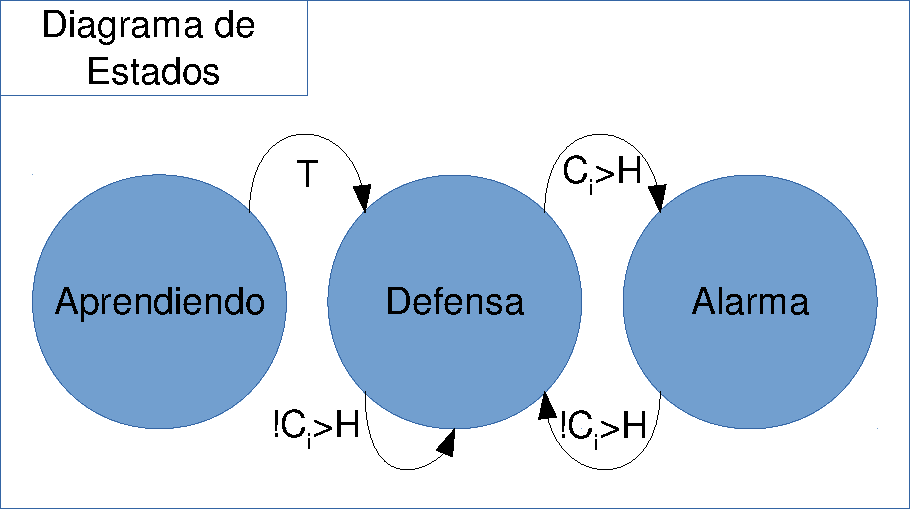
\includegraphics[width=0.6\textwidth]{CapituloCusum/Figuras/DiagramaEstados-crop}
\caption{Diagrama de estados del sensor}
\LABFIG{diagrama_estados} 
\end{figure}
%

\subsection{Periodo de Aprendizaje}\LABSSEC{Periodo de aprendizaje}\index{Periodo de Aprendizaje}
Para poder aplicar el algoritmo CUSUM, es necesario conocer la media y la desviación cuadrática de cada parámetro en el 
tráfico que estamos analizando. Sin embargo, como ya hemos dicho en la introducción de esta sección, es imposible saber 
a priori qué media o qué desviación deben tener dichos parámetros. Se hace necesario un periodo de aprendizaje, en el 
que extraigamos del tráfico dichos estadísticos.

En este periodo de aprendizaje el sistema de defensa recopila la información descrita en la 
\SSEC{Parametros de interés}, y realiza cada intervalo de tiempo $T$ un muestreo. Tras $N$ intervalos, se puede sacar 
una media $\mu_0$ y una desviación cuatrática $\sigma$ del valor que deben tener dichos parámetros.

Es obligatorio suponer que, durante el periodo de aprendizaje, no ha habido ningún ataque realizado sobre la red 
protegida. De cometerse un ataque sobre la red, este será el tomado como \emph{normal} o \emph{típico}, y las 
características del tráfico legítimo no coincidirán.

Una posible forma de conseguir esto podría ser capturar tráfico en un fichero \gls{PCAP}, comprobar que esté libre de 
ataques, y hacerlo pasar por el sistema de aprendizaje. Tras ello, Se extraerá la media y la desviación típica de dicho 
periodo, y se podrá comenzar con el periodo de defensa.

\subsection{Periodo de defensa}\LABSSEC{Periodo de defensa}\index{Periodo de Defensa}
Tras el periodo de aprendizaje (ver \SSEC{Periodo de aprendizaje}), tenemos unos estadísticos con los que comparar el 
tráfico. Por tanto, podemos detectar ataques: Decimos que estamos en el periodo de defensa.

El funcionamiento básico será el mismo que en el periodo de aprendizaje: Por cada \gls{IP}, registramos los valores 
anteriormente descritos. Tras un intervalo de tiempo, extraemos los parámetros significativos enumerados.

Sin embargo, ahora sí poseemos una media y desviación típica con la que comparar. Por tanto, es posible definir un 
valor $C_{i,\text{IPexterna}}$ para cada parámetro, IP externa e intervalo de tiempo, que permita decidir si estamos o 
no bajo ataque por alguna IP concreta. Por otra parte, se lleva la cuenta de estas características a nivel general, por 
lo que también se podrán detectar ataques realizados a base de clonar el comportamiento normal en muchas direcciones 
\gls{IP} distintas.

Si se produce una alarma, esto es, $C_{i,\text{IP}} > H$ para alguna \gls{IP} o los contadores generales, se pasará al 
Modo Alarma\index{Modo Alarma}\index{Modo Alarma}. 

\subsubsection{El aprendizaje durante el periodo de defensa}

Durante el periodo de defensa, es necesario seguir aprendiendo. Por ejemplo, si la media da un valor bajo para los 
paquetes \gls{UDP}, y un cliente sólo se dedica a hacer consultas \gls{UDP} legítimas, es posible que este alcance muy 
pronto el valor umbral para el ratio \gls{UDP}, lo que provocaría una falsa alarma. Por tanto, ante cada nueva IP de la 
que se tengan datos, será necesario hacerla pasar por un tramo de aprendizaje, de forma que se pueda comparar consigo 
misma a lo largo del tiempo.

Por otra parte, si el periodo de aprendizaje ha caído en una hora valle del tráfico, el funcionamiento normal será 
identificado rápidamente como un ataque. Así pues, tras el periodo de aprendizaje original, se realizará otro periodo 
de aprendizaje provisional. Si no se producen alarmas durante este periodo, los nuevos valores \emph{normales} pasarán 
a ser los aprendidos.

\subsubsection{Protocolo de actuación ante un ataque. Modo Alarma}

Ante un ataque, podríamos actuar de tres formas distintas \cite{Raghavan}:
\begin{enumerate}
 \item\emph{Detener el tráfico atacante}, aceptando el riesgo de detener también tráfico legítimo.
 \item\emph{Frenar el tráfico atacante}, lo cual requiere una capacidad de procesamiento mayor por parte del sistema de 
filtrado, que podría llevar a una respuesta mas lenta.
 \item\emph{Aprovisionamiento de recursos}, lo cual puede o puede no ser posible en ese momento.
\end{enumerate}

De las anteriores opciones, la más usada es la de frenar completamente el tráfico considerado como atacante, ya que es 
la que estamos seguros que siempre se podrá llevar a cabo sin afectar negativamente al rendimiento.

Así pues, ante un ataque, el primer paso será dejar de admitir flujos provenientes de direcciones \gls{IP} que no 
hayan sido previamente registradas, de forma que se reduzca el flujo de información hacia el servidor. Esto puede dejar 
fuera conexiones legítimas, pero el permitir nuevas conexiones podría ser aprovechable para continuar machacando el 
servicio.

Tras ello, es necesario inspeccionar, si las hubiese, qué flujos \gls{IP} han ocasionado que salte la alarma, mediante 
el algoritmo \gls{CUSUM} aplicado a cada uno. Se seguirán deteniendo los flujos hasta que, mediante el algoritmo 
\gls{CUSUM} de nuevo, se detecte que estamos fuera de la zona de alerta.

\section{Resumen}%%%%%%%%%%%%%%%%%%%%%%%%%%%%%%%%%%%%%%%

\begin{Resumen}[Resumen del capítulo]
\subsection*{El algoritmo CUSUM}
\begin{displaymath}
\begin{cases}
 \text{control de procesos}
 \begin{cases}
  \text{Diferencia las las pautas \emph{normales} y las \emph{desviaciones}}\\
  \text{Diferencia procesos \emph{bajo control} y \emph{fuera de control}}   \\
  \text{Podemos usarlo para distinguir tráfico legítimo del atacante}
 \end{cases}\\\\

 \text{CUSUM}
 \begin{cases}
  \text{-- SCP con memoria: Detecta pequeñas variaciones a lo largo de mucho tiempo} \\ 
  \qquad x_1,x_2,x_3... \Rightarrow f(x_1),f(x_1,x_2),f(x_1,x_2,x_3)... \\
  \qquad C_1 = (x_1 - \mu_0) \\
  \qquad C_i = C_{i-1} + \left(x_i-\mu_0\right) \\
  \text{-- Se le añade un umbral de sensibilidad $K = K(\sigma)$}\Rightarrow\text{Cambios pequeños no afectan} \\
  \qquad C_i^+ = max\left[0, C_{i-1} + \left(x_i-\mu_0\right)- K\right]\\
  \qquad C_i^- = max\left[0, C_{i-1} - \left(x_i-\mu_0\right)- K\right]\\
  \text{-- Alarma si $C_i$ supera un valor $H = H(\sigma)$} \\
 \end{cases}
\end{cases}
\end{displaymath}

\subsection*{Cusum aplicado al control del tráfico}
\begin{displaymath}
 \begin{cases}
  \text{Parámetros de interés}
  \begin{cases}
   \text{Densidad de conexiones en un sentido} \\
   \text{Longitud media de paquetes} \\
   \text{Relación entre paquetes entrantes y salientes} \\
   \text{Porcentaje de paquetes \gls{TCP}} \\
   \text{Porcentaje de paquetes \gls{UDP}} \\
   \text{Porcentaje de paquetes \gls{ICMP}} \\
   \text{Porcentaje de paquetes LAND (ip origen = ip destino)}
  \end{cases}\\\\
  \text{Periodo de aprendizaje}
  \begin{cases}
   \text{Necesario debido a que no conocemos $\mu_0$ ni $\sigma$ del tráfico} \\
   \text{Acumulación de muestras para conocer dichos parámetros durante un tiempo} \\
   \text{Se supone que no han habido ataques durante el periodo de aprendizaje}
  \end{cases}\\\\
  \text{Periodo de defensa}
  \begin{cases}
   \text{Aplicamos el algoritmo \gls{CUSUM} al tráfico analizado} \\
   \text{Si alguna \gls{IP} o los contadores generales superan $H$, se entra en modo defensa} \\
   \text{Modo defensa}
   \begin{cases}
    \text{Bloqueo de nuevas \gls{IP}} \\
    \text{Búsqueda y bloqueo de IP maliciosas ($C_{i,\text{IP}} > H$).}
   \end{cases}
  \end{cases} \\
 \end{cases}
\end{displaymath}


\end{Resumen}


%
% !TEX root =../LibroTipoETSI.tex
\chapter{Estructura de \redborderddos}\LABCHAP{CAPEstructura}
\pagestyle{esitscCD}
% TODO Falta epígrafe
\epigraph{  FaltaFalta }{FaltaFalta}

%\lettrine[lraise=0.7, lines=1, loversize=-0.25]{E}{l} 
\lettrine[lraise=-0.1, lines=2, loversize=0.25]{R}edBorder DDoS\index{RedBorder DDoS} es el nombre del producto en el 
que, mediante el análisis del tráfico en tiempo real a través del algoritmo \gls{CUSUM}, nos permite detectar ataques 
\gls{DDoS} en tiempo real.

A lo largo de este capítulo, %TODO

\section{Alcance de \redborderddos} %TODO hablar de la escalabilidad.
Como vimos en el \CHAP{Denegacion de Servicio}, podemos diferencias los ataques de \gls{DDoS} en dos grandes bloques: 
Ataques por inundación, que buscan saturar los recursos de los que depende el servicio, y ataques semánticos. que 
buscan explotar una vulnerabilidad conocida.

\redborderddos{} intenta detectar y, en la medida de lo posible, mitigar el primer tipo de ataque, mediante el 
algoritmo \gls{CUSUM} visto en el capítulo \CHAP{Algoritmo CUSUM}. 

%TODO Falta. Relacioanr con los tipos de ataques de DDoS
\section{Nociones previas}

%TODO por qué basado en C

A lo largo de este capítulo se describirá la estructura de \redborderddos. \redborderddos{} está basado en el lenguaje 
de programación C, y usa alguna característica avanzada que no todos los usuarios de C tienen por qué conocer antes de 
leer este capítulo.

Por tanto, describiremos en esta sección las técnicas usadas, a fin de que podamos hacer referencia a ellas al 
describir el funcionamiento del programa sin necesidad de mezclar detalles de bajo y alto nivel.

\subsection{Comparación de números en coma flotante}\index{Número en coma flotante}
Salvar un número decimal en la memoria de un ordenador tiene una condición importante: La memoria del ordenador es 
finita. Los números, por el contrario, son infinitos. Es más, entre dos números distinguibles cualesquiera, hay 
infinitos números reales intermedios.

Así, pues, si destinamos por ejemplo $4$ bits de memoria para guardar un número, para una misma base sólo podremos 
guardar $2^{4}$ números distintos. Si, por ejemplo, queremos guardar los números posibles entre $0$ y $1$, la 
asignación número $\rightarrow$ representación binaria quedaría como en la \TAB{RepresentacionBinariaEjemplo4bits}.

\begin{table}
\begin{tabular}{cl}
 Representación & Número \\\hline
  \texttt{0000} & 0.000000 \\
  \texttt{0001} & 0.066667 \\
  \texttt{0010} & 0.133333 \\
  \texttt{0011} & 0.200000 \\
  \texttt{0100} & 0.266667 \\
  \texttt{0101} & 0.333333 \\
  \texttt{0110} & 0.400000 \\
  \texttt{0111} & 0.466667 \\
  \texttt{1000} & 0.533333 \\
  \texttt{1001} & 0.600000 \\
  \texttt{1010} & 0.666667 \\
  \texttt{1011} & 0.733333 \\
  \texttt{1100} & 0.800000 \\
  \texttt{1101} & 0.866667 \\
  \texttt{1110} & 0.933333 \\
  \texttt{1111} & 1.000000
 \end{tabular}
 \caption{Representación posible de flotantes equidistantes desde el 0 hasta el 1 usando cuatro bits.}
 \LABTAB{RepresentacionBinariaEjemplo4bits}
\end{table}

Si, con esta representación, computamos $1/4+1/4-1/2$, el ordenador tendría que aproximarlo a 
$\mathtt{0b0100}+\mathtt{0b0100}-\mathtt{0b0111} \rightarrow 0.266667+0.266667-0.466667$, las representaciones más 
próximas de las que disponemos. Entonces, el resultado de la operación binaria sería $\mathtt{0b0001} \rightarrow 
0.066667$, y no $0$, como se esperaría en un sistema numérico real.

Pese a que en el proyecto se trabaja con números en punto flotante IEE754 dobles, capaces de almacenar $2^64$ números 
distintos, no estamos exentos de este tipo de fallos. Para evitarlos, la comparación entre números no debe ser 
realizada con el operador \texttt{==}, sino que en su lugar se compararán dejando lugar a un margen de error, como se 
ve en Algoritmo \ALG{ComparacionFlotante}.

\begin{algorithm}
 \KwData{Dos números $n_1$,$n_2$ en formato \texttt{double IEEE754}, y un epsilon $e$}
 \KwResult{Comparación de los mismos: 0 si son iguales, $>0$ si $n_1>n_2$ y $<0$ en otro caso}
 \eIf{$abs\left(n_1-n_2\right)< e$}{
   devolver 0\;
 }{
   devolver $n_1-n_2$\;
 }
 \caption{Algoritmo de comparación de números en punto flotante}
 \LABALG{ComparacionFlotante}
\end{algorithm}


\subsection{Estructuras de datos básicas}\index{Estructura de datos}
Para almacenar el funcionamiento de cada flujo de tráfico, y ser capaz de compararlo con el supuesto funcionamiento 
normal de la red, es necesario contar con unos sistemas de almacenamiento rápidos y eficientes. Si se pierde demasiado 
tiempo en el manejo de la memoria, \redborderddos{} no será capaz de leer y modelar el tráfico a una velocidad 
correcta, y a la larga no será capaz de detectar nada.

A lo largo de esta subsección describiremos las estructuras de almacenamiento de datos usadas en el programa. Una vez 
que conozcamos el funcionamiento de estas, será más fácil ver el sistema como un todo, y abstraer correctamente cada 
una de sus partes.

\subsubsection{Vector de memoria}\index{Vector}\LABSSSEC{VectorMemoria}
Un vector consiste en una o más celdas de memoria situadas de una forma contigua. Esto es, si cada elemento del vector 
ocupa $L$ bytes, y el vector comienza en la dirección de memoria $M$, podemos acceder al tercer elemento del vector en 
la dirección $M+3L$.

El vector tiene un tamaño fijo conocido en el momento de su creación, y, a lo largo de este trabajo, no variará. Hemos 
de tener precaución al acceder a las distintas posiciones del vector: si hemos reservado memoria para $K$ elementos, y 
accedemos al elemento número $J>=K$\footnote{En C, las posiciones del vector empiezan en 0. Si accedemos al elemento 
$K$, ya estamos accediendo a memoria fuera del vector}, esa zona de memoria no está dentro del vector, y no se puede 
saber qué habrá.

\subsubsection{Listas enlazadas}\index{Lista Enlazada}\LABSSSEC{ListaEnlazada}
Si, tras haber definido un tamaño de vector, queremos añadir nuevos elementos, deberíamos redimensionar el espacio 
reservado del vector en memoria. Esta es una operación costosa, ya que puede no existir espacio contiguo al final o 
principio del vector, y necesitar buscar un espacio contiguo más grande. Tras encontrarlo, se necesitará copiar todos 
los elementos del vector, y pueden ser muchos.

Aún peor, ¿qué ocurre cuando queremos insertar un elemento en mitad del vector? Es necesario mover todos los elementos 
desde la posición requerida hasta el final del vector una unidad, y después insertar ese último elemento, lo que 
resulta inadmisible.

% TODO describir NULL en el glosario?
Para solucionar este problema, podemos usar una lista tipo enlazada. En ella, cada elemento tiene un puntero que apunta 
al siguiente elemento, mientras que el último elemento de la lista siempre apuntará a NULL. Por lo tanto, insertar o 
eliminar un elemento en mitad de la lista sólo requeriría localizar el elemento anterior, y modificar dos puntero. Como 
caso especial está el insertado de elementos a la cabeza de la lista, que sólo requiere modificar dos punteros.

Podemos ver en la \FIG{EstructuraLinkedList} la estructura que tendría.

\begin{figure}[htbp]
\centering
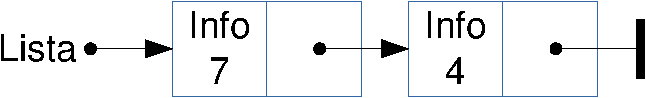
\includegraphics[width=0.5\textwidth]{CapituloEstructura/Figuras/EstructuraListaEnlazada-crop}
\caption{Estructura de una lista enlazada}
\LABFIG{EstructuraLinkedList} %Esto es una forma propia de los autores de gestionar las etiquetas y referencias
\end{figure}
%

Sin embargo, el acceso aleatorio a un elemento de la lista enlazada es algo más costoso, ya que para acceder la 
posición $N$ es necesario iterar por todos los $N-1$ elementos. Existen otras variantes, que incluyen usar un puntero 
al anterior y posterior nodo, listas circulares, listas con puntero a la cabeza y a cola, etc. Pero por el momento, nos 
basta con esta visión de las listas enlazadas.

%TODO explicar listas doblemente enlazadas, y la lista tommy.

\subsubsection{Pilas}\index{Pila}
Una pila es una estructura de datos con sólo dos operaciones: añadir elementos a la pila (operación \emph{push}) y 
extraer el último elemento de la pila (operación \emph{pop}). Si insertamos un elemento $E$, insertamos tras él $N$ 
elementos, será necesario extraer (\emph{pop}) los $N$ elementos antes de volver a acceder al elemento $E$. Es, por 
tanto, una cola \gls{LIFO}.

Podemos simular una pila con un vector de memoria, si llevamos la cuenta de los elementos que hemos insertado con una 
variable \emph{cuenta} con valor inicial a cero, podemos hacer \emph{push} salvando en dicha posición e incrementando 
esa variable, y \emph{pop} decrementandola y devolviendo la posición.

\subsubsection{Tabla HASH}\index{Tabla HASH}
Resumiendo los apartados \SSSEC{VectorMemoria} y \SSSEC{ListaEnlazada}:
\begin{itemize}
 \item Es muy rápido acceder a una posición dada de un vector, pero la inserción de elementos es potencialmente muy 
lenta. Además, mientras el vector no está lleno, desperdicias memoria
 \item El acceso aleatorio a un elemento de una lista enlazada es lento. Sin embargo, la inserción de elementos en 
cualquier punto es rápida, especialmente al principio, y no se desperdicia memoria.
\end{itemize}

La tabla HASH pretende aunar lo mejor de ambas estructuras. Una tabla HASH es un mapa asociativo, en el que cada 
\emph{valor} $V$ tiene asociada una \emph{clave} $K$ por la que puede ser buscado, y dicha clave determina una posición 
en un vector de memoria.

Internamente, el vector de memoria tiene $S$ posiciones, donde $S$ es una potencia de 2.Cada posición es una lista de 
elementos del mismo tipo que el valor que queremos almacenar.

\begin{figure}[hbtp]
\centering
%\hfill
\subfloat[Diagrama de Actividad de Inserción]%
   {\LABFIG{InsertarTablaHash}%
   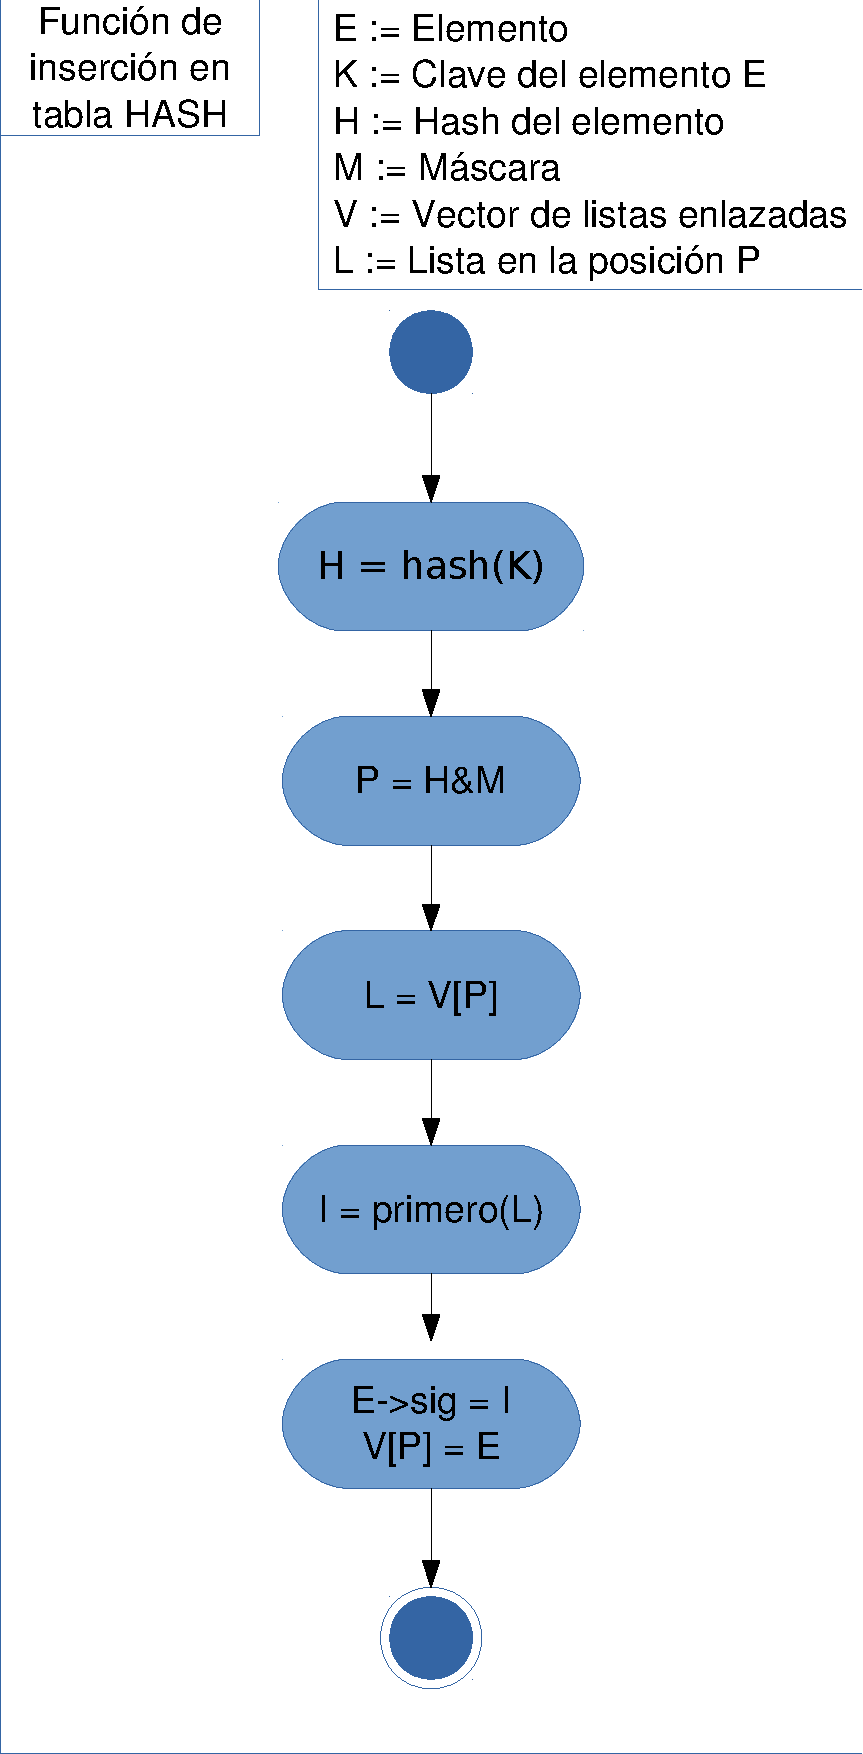
\includegraphics[width=0.48\textwidth]{CapituloEstructura/Figuras/ActividadFuncionInsertarTablaHash-crop}}%
\hfill
\subfloat[Diagrama de actividad de Búsqueda]%
 {\LABFIG{BuscarTablaHash}%
 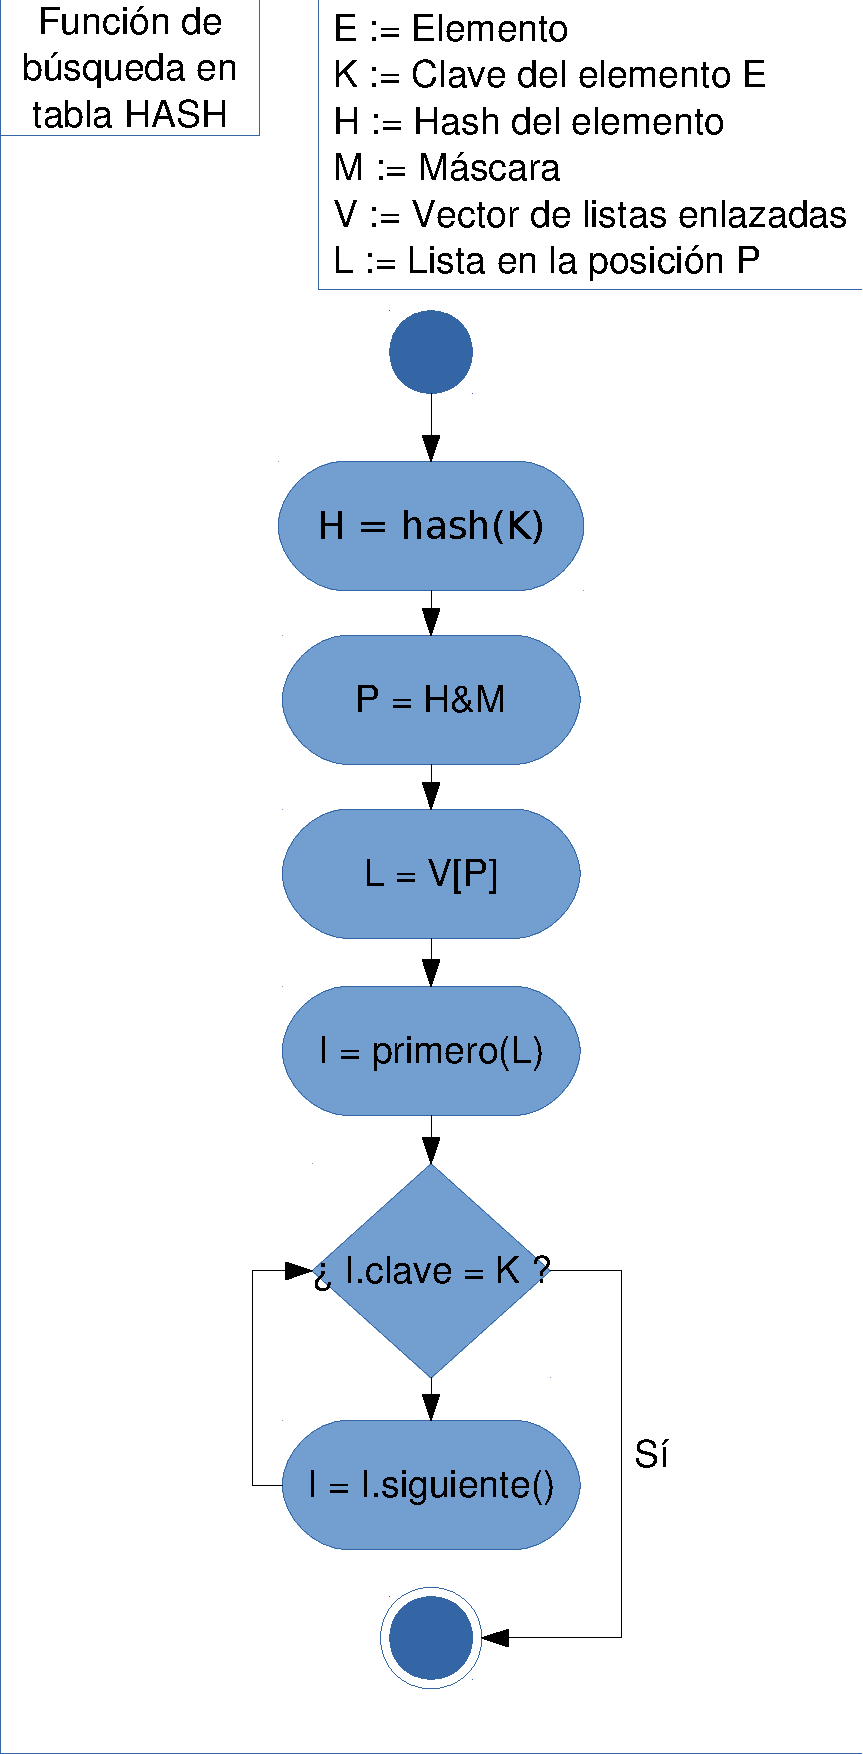
\includegraphics[width=0.48\textwidth]{CapituloEstructura/Figuras/ActividadFuncionBuscarTablaHash-crop}}%
%
\caption{Diagrama de Actividad de las operaciones a realizar sobre una tabla HASH}
\end{figure}
%

A la hora de almacenar un elemento $E_0$ con clave $K_0$, a la clave se le aplica una máscara que asegure un número 
inferior a $S$: Por ejemplo, si $S$ es $2^8$, la máscara debe ser $M=0xff$, de forma que la operación \emph{AND} bit a 
bit de siempre $P_0=K_0\&S<2^8$. El elemento $E_0$ es entonces insertado en la lista que ocupa la posición $P_0$ del 
vector de memoria. El diagrama de actividad de esta función se puede ver en \FIG{InsertarTablaHash}.

Por su parte, a la hora de recuperar el elemento, volvemos a aplicar la máscara a la clave, $P_0=K_0\&M$, y buscamos en 
la lista enlazada que ocupa la posición $P_0$ del vector. Esta vez, sí deberemos comparar los elementos con la clave 
$K$, ya que en ella existen todos los elementos insertados cuyas claves $K$ cumplan $K\&M=P_0$. Podemos ver su diagrama 
de actividad en \FIG{BuscarTablaHash}.

Para conseguir la mínima probabilidad de colisión, se le aplica a las diferentes claves una función HASH\index{Función 
HASH}, esto es una, función que ante la misma entrada de siempre la misma salida, pero que pequeñas diferencias de los 
valores de la entrada provoca grandes diferencias en los valores de salida. Como nota, es probable que una función HASH 
produzca colisiones, esto es, diferentes entradas producen la misma salida.

En el mismo sentido, es importante encontrar una buena relación entre el tamaño de la tabla hash y el número de 
elementos que queremos insertar. Siempre será más rápido que una lista puramente enlazada, pero cuantos menos elementos 
ocupen la misma posición de memoria, mejor.

%TODO reservar una sección "pruebas realizadas"

Por ejemplo, supongamos que queremos almacenar unos contadores, cuyo flujo está asociado a la \gls{IP} \emph{10.0.1.1}, 
en una tabla hash de longitud $S=2^8$. Tras aplicarle nuestra función HASH, vemos que 
$\text{hash}(\text{10.0.0.1})=476$. Buscamos en la tabla HASH la lista enlazada de la posición 
$476\&0xff=220$, y la añadimos a la cola. Ver \FIG{EstadoTablaHashInsercion} para visualizar gráficamente qué ocurre 
con la tabla HASH.

\begin{figure}[hbtp]
\centering
\subfloat[Estado antes de la inserción]%
   {\begin{minipage}[t]{0.47\textwidth}\vspace{0pt}
    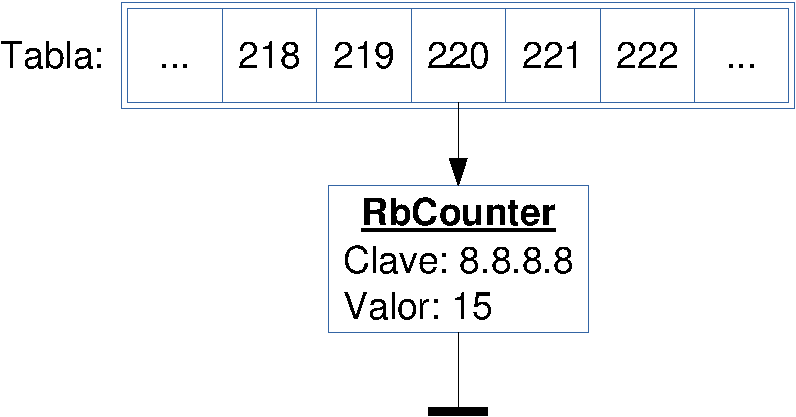
\includegraphics[width=\textwidth]{CapituloEstructura/Figuras/TablaHashAntesInsercion-crop}%
    \end{minipage}}
\hfill
\subfloat[Estado después de la inserción]%
 {\begin{minipage}[t]{0.47\textwidth}\vspace{0pt}
 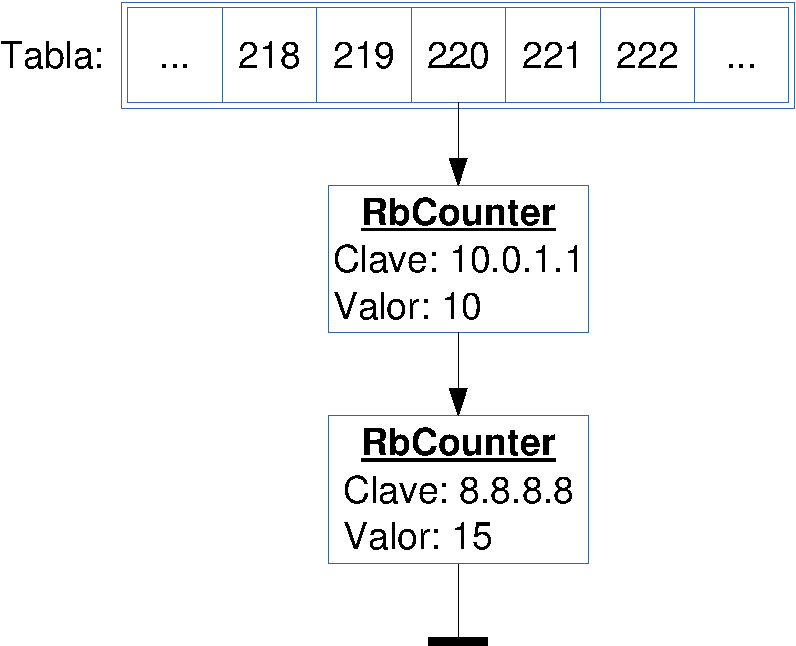
\includegraphics[width=\textwidth]{CapituloEstructura/Figuras/TablaHashDespuesInsercion-crop}%
  \end{minipage}}
%
\caption{Inserción de un elemento en la tabla HASH}
\LABFIG{EstadoTablaHashInsercion}
\end{figure}

\subsection{Programación multihilo}\LABSSEC{ProgramacionMultihilo}
Un hilo de un proceso\index{Hilo}, también llamado proceso ligero\index{Proceso Ligero}, es una forma que tienen las 
aplicaciones de ejecutar código de manera concurrente. 

Al crear un hilo, se crea una nueva entrada en el planificador\index{Planificador} del \gls{SO}, y ésta instancia se 
ejecutará con la misma prioridad que otros procesos. Tendrá su propio contador de programa\footnote{Indicador del punto 
de ejecución actual.}, su propia pila de llamada a funciones y su propio estado de CPU, lo que permite que el hilo 
llamante y el llamado se ejecuten por separado.

Sin embargo, los distintos hilos de un proceso comparten el espacio de direcciones y ficheros abiertos. Esto es útil 
para compartir memoria entre ellos, pero genera la necesidad de un mecanismo de sincronización.

Por ejemplo, supongamos una función que realiza las siguientes acciones sobre un entero de valor 0:
\begin{enumerate}
 \item Copia un entero a un registro\label{item:EjemploHilosGetInt}.
 \item Incrementa ese entero.
 \item Vuelve a guardar ese entero en su ubicación original, ya incrementado.
\end{enumerate}

Esta función se está llamando concurrentemente\index{Concurrencia} desde dos hilos distintos. Se debería esperar que, 
tras la ejecución de los dos hilos, el entero valga 2.

Sin embargo, si hilamos mas fino, descubrimos un problema. Pongamos el caso de que, en el momento de terminar la 
instrucción \ref{item:EjemploHilosGetInt}, el planificador decide que es hora de pasar el control al hilo dos. 
Éste lee la variable (de valor 0), la incrementa, y guarda un 1. Ahora, cuando el control vuelve al hilo 1, este 
simplemente tiene en su registro un 0, lo incrementará a 1, y guardará un 1. Y no podemos saber cuando el planificador 
decidirá cambiar el hilo en ejecución, por lo que este problema se puede reproducir de manera aleatoria.

Es necesaria una \emph{Variable Cerrojo}\index{Variable Cerrojo}\index{Mutex}. Una variable especial que sólo puede ser 
modificada por un proceso al mismo tiempo en todo el sistema y, por tanto, proteja la \emph{sección 
crítica}\index{Sección Crítica}, esto es, aquella susceptible de ser indeterminada si el procesador cambia de hilo de 
ejecución en el momento que está siendo ejecutada.

Por tanto, la función pasaría a ser:
\begin{enumerate}
 \item Cerramos la variable cerrojo
 \item Copia un entero a un registro
 \item Incrementa ese entero.
 \item Vuelve a guardar ese entero en su ubicación original, ya incrementado.
 \item Abrimos la variable cerrojo
\end{enumerate}

De esta forma, ambos hilos de ejecución saben cuando otro proceso está modificando la \emph{región crítica}.

No obstante, esto tiene una desventaja: el hilo que espera a que la variable cerrojo sea abierta no puede hacer otra 
cosa que no sea esperar. Por tanto, una mala elección de secciones críticas hará el programa lento.

\subsection{Señales en linux. La señal SIGALRM.}\LABSSEC{SIGALRM}\index{SIGALRM}\index{Señal Linux}
Un mecanismo de comunicación entre procesos o \gls{IPC} es el envío de señales. Por ejemplo, cuando un programa intenta 
escribir en un área de memoria restringida, el \gls{SO} le envía una señal \gls{SIGSEGV}, y el proceso puede actuar en 
consecuencia.

Cuando un proceso la recibe, pueden ocurrir tres cosas según la señal. Por defecto, o es ignorada, o abortará el 
programa. No obstante, también es posible escribir código para manejar algunas señales.

En este caso, cuando el proceso decida crear un manejador para una señal\index{Manejador de señal Linux} concreta, y 
reciba dicha señal, será interrumpido y será como si en ese momento hubiese llamado al manejador. Cuando el manejador 
termine, el programa seguirá su ejecución normal. Si el programa estaba en un \texttt{sleep}, este será interrumpido, y 
el programa no dormirá los segundos restantes.

Por ejemplo, si pulsamos \texttt{Ctrol-Z} en un programa, este detendrá su ejecución y podremos o bien enviarlo a 
segundo plano con el comando \texttt{bg} o reanudar su ejecución con \texttt{fg}. Esto es notificado al programa con 
una señal \gls{SIGTSTP}, y es posible manejarla.

Por ejemplo, el \lstlistingname{} \ref{code:dumbSignalStopHandling} muestra un ejemplo de manejo de esta señal. Sin 
embargo si varias señales llegan muy rápido, comenzaremos a manejar una señal mientras aún estábamos manejando la 
anterior, por lo que tenemos el mismo problema que en \SSEC{ProgramacionMultihilo}. Para colmo, no podemos solucionarlo 
con una variable cerrojo: \gls{pthreads}\index{Librería phtread} establece que el resultado de bloquear una señal 
bloqueada por tu mismo hilo de ejecución es indeterminado. Y esto podría pasar si el manejador de la señal salta en la 
región crítica.

\begin{lstlisting}[language=C++,caption={Manejo ingenuo de la señal \gls{SIGTSTP}}, 
breaklines=true, label=code:dumbSignalStopHandling,numbers=left,float=htbp]
#include <signal.h>
#include <stdio.h>

#define N 10
static int i = 0;
static int salir = 0;

static void manejador(int signo){
    if(i++<N)
        printf("¡No quiero parar!\n");
    else
        salir = 1;
}

int main(void) {
     signal(SIGTSTP, manejador);
     while (!salir)
         sleep(1);
     return 0;
}
\end{lstlisting}

Así pues, la solución pasa por reducir al mínimo la responsabilidad del manejador de la señal: Este sólo establecerá un 
indicador global de que la señal ha sido recibida, y el manejador real estará en un hilo y, por tanto, en un entorno 
controlado. Vemos un ejemplo de este modo de proceder en \lstlistingname{} \ref{code:SignalStopHandling}

\begin{lstlisting}[language=C++,caption={Manejo de la señal \gls{SIGTSTP}}, 
breaklines=true, label=code:SignalStopHandling,numbers=left,float=htbp]
#include <signal.h>
#include <stdio.h>

#define N 10
static int sig = 0;

static void manejador(int signo){
    sig = 1;
}

int main(void) {
     int i = 0;
     signal(SIGTSTP, manejador);
     while (i<N){
        sleep(1);
        if(sig){
            printf("¡No quiero salir!\n");
            ++i;
            sig = 0;
        }
    }
    return 0;
}
\end{lstlisting}

Por último, una señal interesante, y que usaremos en el proyecto, es la señal \gls{SIGALRM}\index{Señal 
\texttt{SIGALRM}}. Mediante la función \texttt{alarm(int s)}\index{Función \texttt{alarm}}, se le notifica al \gls{SO} 
de que se desea recibir una señal \gls{SIGALRM} pasados \texttt{s} segundos. Por tanto, se podría usar para realizar 
tareas periódicas. Por ejemplo, el \lstlistingname{} \ref{code:AlarmSignal} imprimirá la fecha actual\footnote{En 
formato \emph{UNIX time}\index{UNIX time}, esto es, segundos transcurridos desde el 1 de Enero de 1970} y un mensaje 
indicativo de que se está realizando alguna tarea.

\begin{lstlisting}[language=C++,caption={Ejemplo de uso de \gls{SIGALRM}}, 
breaklines=true, label=code:AlarmSignal,numbers=left,float=htbp]
#include <signal.h>
#include <stdio.h>
#include <time.h>   // time()
#include <unistd.h> // alarm()

static int alarma = 0;

static void manejador(int signo){
    alarma = 1;
    alarm(1); // Programamos la siguiente alarma
}

int main(void) {
     signal(SIGALRM, manejador);
     alarm(1);
     while (1){
        sleep(1);
        if(alarma){
            printf("[%d] Estoy haciendo cosas...\n",time(NULL));
            // Sleep(100)
            alarma = 0;
        }
    }
    return 0;
}
\end{lstlisting}

Sin embargo, este programa vuelve a ignorar la concurrencia. ¿Qué ocurre si el programa tarda mas de la cuenta en 
ejecutarse? Si des-comentamos el \texttt{sleep(100)} entre el \texttt{printf(...)} y el \texttt{alarma = 0}, vemos que 
el programa imprime el mensaje cada dos segundos, en lugar de cada segundo. Esto es debido a que se ha lanzado la 
alarma mientras se estaba ejecutando el trabajo (el \texttt{sleep}), y nada ha cambiado tras ello (ya que sólo hemos 
establecido \texttt{alarma} a 1, pero ya estaba a 1). Debido a ello, es posible que el trabajo no se esté ejecutando 
con la periodicidad que nosotros creemos.

Para solucionarlo, se hace necesario otra variable que indique que una señal ha llegado mas tarde de la cuenta. En 
\lstlistingname{} \ref{code:AlarmSignalAcumulados}. 

Por último, no se debe confiar en hacer de \texttt{acumulados} un contador, ya que la alarma podría saltar en cualquier 
momento entre el \texttt{if(acumulados)} y el \texttt{acumulados=0}. Es necesario confiar en otros sistemas, como 
almacenar la marca de tiempo en la que el proceso fue lanzado.

\begin{lstlisting}[language=C++,caption={Ejemplo de uso de \gls{SIGALRM} con detección de pérdidas}, breaklines=true, 
label=code:AlarmSignalAcumulados,numbers=left,float=htbp]
#include <signal.h>
#include <stdio.h>
#include <time.h>   // time()
#include <unistd.h> // alarm()

static int alarma = 0;
static int acumulados = 0;

static void manejador(int signo){
    if(alarma)
        acumulados = 1; // Aún no ha acabado el anterior trabajo
    alarma = 1;
    alarm(1); // Programamos la siguiente alarma
}

int main(void) {
     signal(SIGALRM, manejador);
     alarm(1);
     while (1){
        sleep(1);
        if(alarma){
            if(acumulados){
                printf("[%d] Nos hemos saltado alguna iteración.",time(NULL));
                printf(" Se actuará en consecuencia.\n");
                acumulados = 0;
            }
            printf("[%d] Estoy haciendo cosas...\n",time(NULL));
            sleep(100);
            alarma = 0; // Todo vuelve a la normalidad
        }
    }
    return 0;
}
\end{lstlisting}

\section{Vista externa}\LABSEC{Vista Externa}
\subsection{Situación física de \redborderddos}
Desde el punto de vista de la arquitectura de red, \redborderddos{} debe colocarse en dos puertos SPAN\index{Puerto 
SPAN} del conmutador que llegue al activo protegido, tal y como muestra la \FIG{diagramaArquitectura}. Cada uno de los 
puertos SPAN clonará los paquetes dirigidos hacia el activo a proteger, y los paquetes desde el activo a proteger 
respectivamente, y los enviará hacia \redborderddos.

\begin{figure}[htbp]
\centering
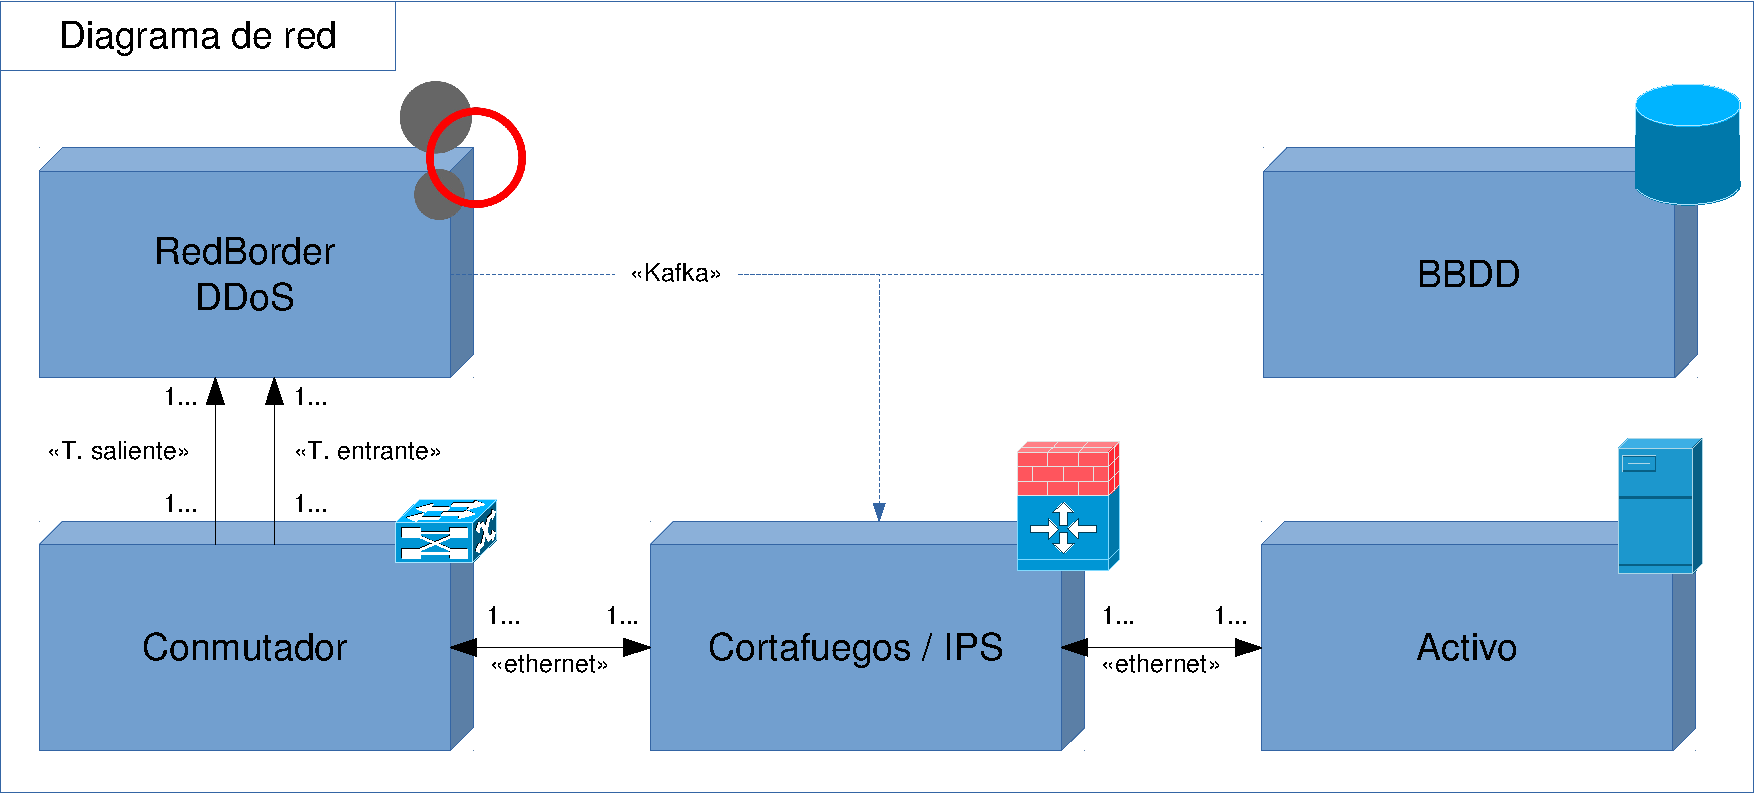
\includegraphics[width=\textwidth]{CapituloEstructura/Figuras/DiagramaArquitectura-crop}
\caption{Diagrama de Arquitectura de \redborderddos}
\LABFIG{diagramaArquitectura} %Esto es una forma propia de los autores de gestionar las etiquetas y referencias
\end{figure}
%

Tras el conmutador, se debería colocar un cortafuegos o \gls{IPS}, que se usa para:
\begin{enumerate}
 \item Detener el tráfico detectado como atacante por \redborderddos.
 \item Detener ataques semánticos o usuarios no autorizados.
\end{enumerate}

\redborderddos{} puede funcionar sin el cortafuegos\index{Cortafuegos}. No obstante, en ese caso sólo detectaremos los 
ataques, en lugar de detenerlos efectivamente.

Es necesario que \redborderddos{} se coloque delante del elemento que corta el tráfico. De otra forma, sería imposible 
para el sistema conocer cuándo ha cesado el ataque, y cuándo podemos dejar el Modo Alerta.

Podemos ver en el diagrama que podríamos multiplicar los puertos de SPAN. Esto es, si tenemos demasiado tráfico y no es 
posible enviarlo todo por un sólo puerto, podemos dedicar a \redborderddos{} dos puertos de entrada y dos de salida. 
Incluso, podríamos dedicar dos o más puertos de entrada, y sólo uno de tráfico saliente, si el tráfico que tenemos es 
altamente asimétrico. Cualquier combinación es posible, siempre y cuando tengamos al menos un puerto destinado a cada 
dirección. De esta forma, \redborderddos{} es completamente escalable desde un punto de vista de admisión de datos.

\subsection{Registro y alerta del ataque. El protocolo Apache Kafka}
% TODO ver formato del registro: Disco duro y por kafka
Cuando un ataque se produce, \redborderddos{} es capaz de registrarlo en un fichero de texto plano del disco duro y 
enviarlo por la plataforma Apache Kafka\index{Apache Kafka}.

Apache Kafka es un protocolo de transferencia de mensajes que sigue un modelo de intercambiador o 
\emph{broker}\index{Kafka Broker}. Está diseñado para ser distribuido y extensible \cite{ApacheKafka}, por lo que si 
encontramos mucha carga de trabajo, es posible aumentar, de manera horizontal\footnote{Esto es, doblar el número de 
nodos debe doblar, aproximadamente, el rendimiento obtenido.}, la capacidad de procesamiento, siempre y cuando 
dispongamos de máquinas (reales o virtuales) que sirvan de nodos Kafka.

Así, \redborderddos{} es un productor Kafka\index{Productor Kafka}, que envía el registro de ataques a una cola de 
mensajes a un \emph{broker}, que los almacenará y entregará al consumidor\index{Consumidor Kafka} que los solicite.

Muchos sistemas de procesamiento de eventos usan Apache Kafka como base para su funcionamiento. Por ejemplo, es posible 
enriquecer los eventos con Apache Storm\index{Apache Storm} \cite{ApacheStorm}, o bien almacenarlos en una base de 
datos orientada a documentos como MongoDB\index{MongoDB} \cite{MongoDB}, mucho más rápida a la hora de almacenar este 
tipo de eventos que las bases de datos relacionales usadas tradicionalmente.

\subsection{Mitigación del ataque}
Para mitigar el ataque, es necesario que exista un cortafuegos\index{Cortafuegos} o un \gls{IPS}\index{Intrusion 
Prevention System} que bloquee el tráfico dirigido al activo a proteger. Una vez que éste existe, es necesaria una vía 
de comunicación con el mismo. Actualmente, \redborderddos{} simplemente alerta de los ataques, por lo que sería 
necesario que el \gls{IPS} o algún sistema intermedio leyese de la cola Kakfa y modificase su comportamiento en base a 
dicha lectura.

\section{Estructura general}\LABSEC{EsctructuraGeneral}
Internamente, \redborderddos{} intenta aprovechar al máximo la potencia de procesamiento del sensor, haciendo todas las 
tareas posibles de una manera concurrente.

Para ello, separaremos en distintos núcleos\footnote{Entendidos como núcleos de procesadores físicos.} del sensor los 
distintos bloques funcionales en los que se divide el proyecto, representados en la figura \FIG{diagramaActividad}. A 
saber:

\begin{description}
 \item [Clúster] La función del clúster es agrupar los paquetes entrantes y salientes de las distintas 
interfaces, indicar el sentido del mismo, y dirigirlos a las distintas colas que los sub-contadores leen.
 \item [Sub-contadores] Los sub-contadores agrupan todos los paquetes entrantes por flujos según IP externa, y 
contabilizan los distintos valores necesarios para ejecutar el algoritmo \gls{CUSUM} por cada flujo.
 \item [Contador Maestro y Decisor] El contador maestro, cada periodo de tiempo definido, recoge los contadores de cada 
sub-contador y aplica el algoritmo \gls{CUSUM} sobre ellos. Por su parte, el decisor se encarga de comparar dichos 
valores con los valores límite, identificando la IP como atacante si encontramos que una de ellas los sobrepasa.
\end{description}

\begin{figure}[htbp]
\centering
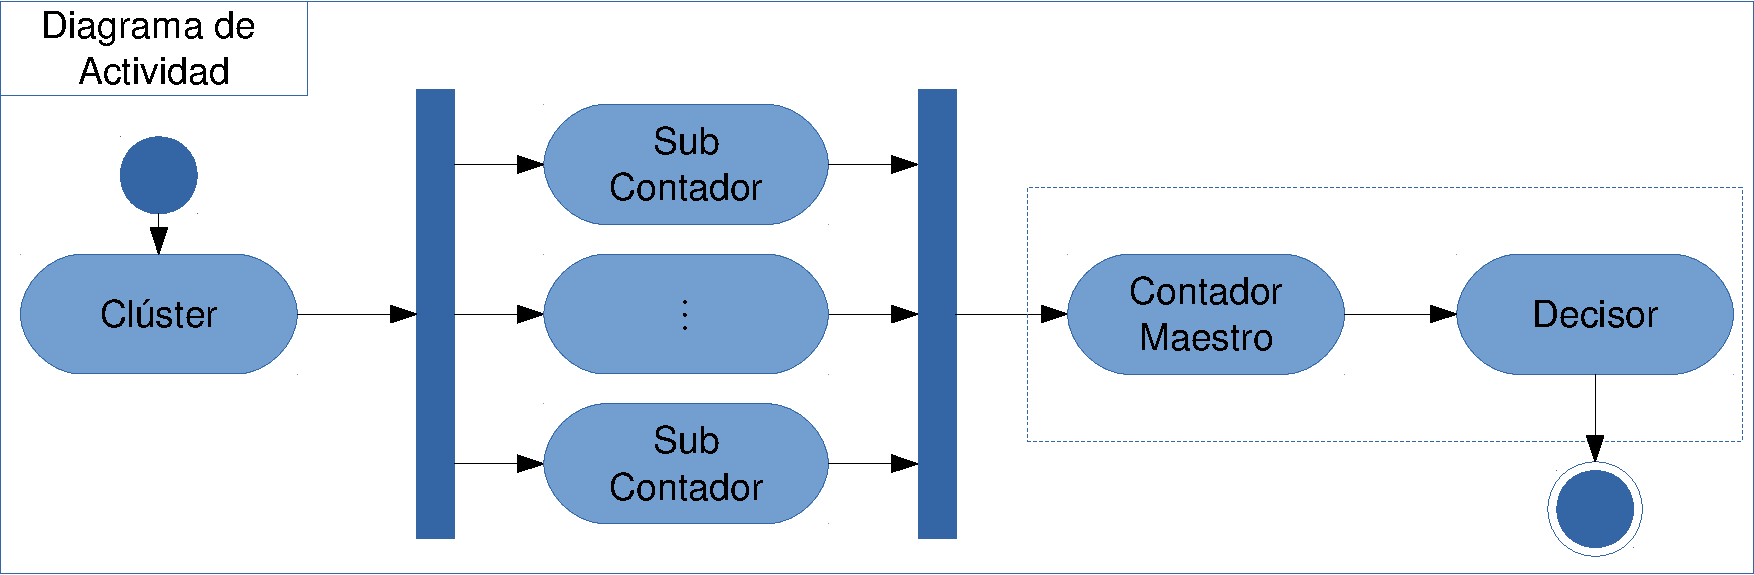
\includegraphics[width=\textwidth]{CapituloEstructura/Figuras/DiagramaFlow-crop}
\caption{Diagrama de Actividad de \redborderddos}
\LABFIG{diagramaActividad}
\end{figure}
%

\subsection{Clúster}\index{PF\_RING Cluster}\LABSSEC{EstructuraCluster}
Un clúster \acrshort{PFRING}\footnote{En el capítulo \CHAP{@TODO} se detallará qué es \acrshort{PFRING}. Por el 
momento, es sólo el nombre concreto de este tipo de clúster.} es capaz de dividir todo el troncal de tráfico recogido 
por una o varias interfaces en una o más colas, de forma que cada cola vea sólo una porción del tráfico, de una manera 
coherente.

\begin{figure}[htbp]
\centering
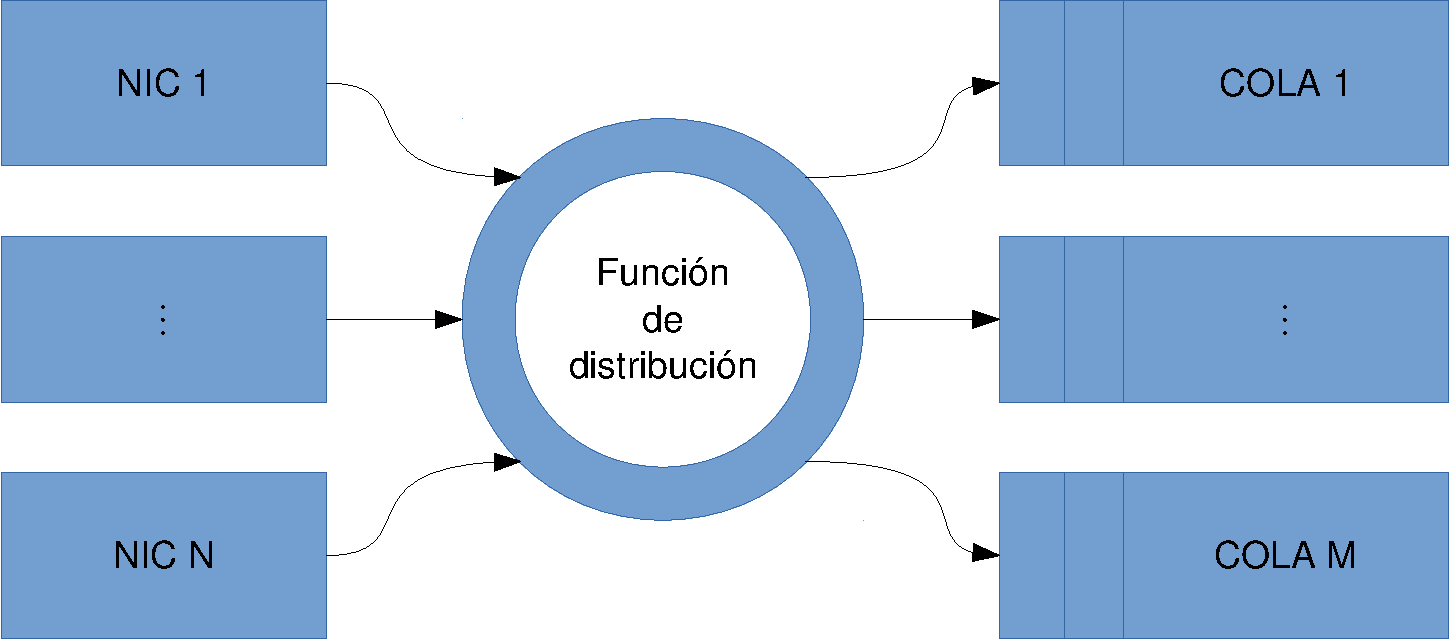
\includegraphics[width=0.75\textwidth]{CapituloEstructura/Figuras/Cluster-crop}
\caption{Funcionamiento del clúster}
\LABFIG{Cluster}
\end{figure}
%

La función de distribución es completamente definible: Podríamos haber decidido enviar los paquetes en 
\emph{round-robbin}, esto es, uno a cada cola cada vez.

La forma de reenvío que hemos elegido es por tupla (\emph{IP origen},\emph{IP destino}) de manera simétrica, esto es, 
la petición y la respuesta de un mismo flujo siempre irá dirigido a la misma cola. De esta forma, como se verá más 
adelante, cada hilo contador (ver \SSEC{subcontadores}) sólo ve una parte del flujo coherente, y el contador maestro, a 
la hora de agrupar todos los flujos, tendrá que hacer muchas menos operaciones, ya que nunca se tendrán que sumar dos 
registros.

Por otra parte, la función de distribución marcará el paquete como entrante o saliente, según haya llegado por una 
interfaz definida como tal.

Al multiplexar de esta forma las colas, conseguimos reducir el número de inter-bloqueos, ya que en 
logar de tener un modelo en el que muchos hilos atacan una misma cola, cada hilo sólo mirará su propia cola,, y en cada 
cola sólo podrán actuar dos bloqueantes (el cluster y el hilo).

De esta forma, conseguimos transparencia y escalabilidad en el número de interfaces de entrada de datos, e 
incrementamos el rendimiento a la hora de agrupar los paquetes.

Se puede ver el gráficamente el algoritmo seguido por la función de distribución en el diagrama de actividad de la 
\FIG{ActividadDistribFunc}.

\begin{figure}[htbp]
\centering
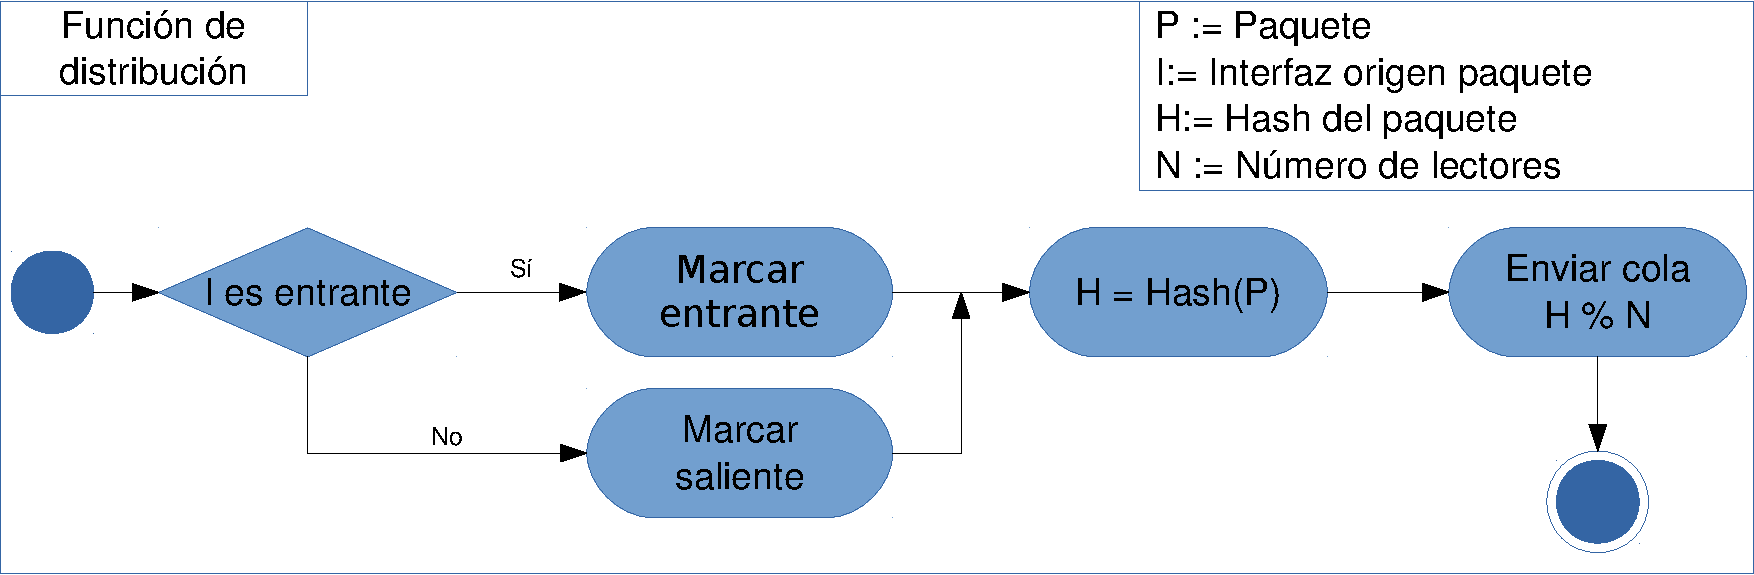
\includegraphics[width=\textwidth]{CapituloEstructura/Figuras/ActividadFuncionDistribucionCluster-crop}
\caption{Función de distribución}
\LABFIG{ActividadDistribFunc}
\end{figure}
%

\subsection{Subcontadores}\index{Subcontador}\LABSSEC{subcontadores}
\subsubsection{Estructura contador}
Con el fin de almacenar las características del tráfico descritas en \SSEC{Parametros de interés}, se prepara una 
estructura de datos en la que se irán contando los paquetes y octetos de cada tipo. Dicha estructura de datos puede 
verse en \lstlistingname{} \ref{code:RbCounter}. Por comodidad, dicha estructura también será llamada, a lo largo del 
proyecto, simplemente \texttt{RbCounter}.

\begin{lstlisting}[language=C++,caption={Estructura de contadores por flujo}, breaklines=true, 
label=code:RbCounter,numbers=left,float=htbp]
typedef uint32_t counter_t;

typedef struct rb_counters_s{
    rb_addr_t external_address; ///< External IP address

    counter_t tcp_pkts;     ///< number tcp packets in the flow
    counter_t udp_pkts;     ///< number udp packets in the flow
    counter_t icmp_pkts;    ///< number icmp packets in the flow
    counter_t total_pkts;   ///< total number packets in the flow

    counter_t tcp_bytes;    ///< tcp bytes in the flow
    counter_t udp_bytes;    ///< udp bytes in the flow
    counter_t icmp_bytes;   ///< icmp bytes in the flow
    counter_t total_bytes;  ///< total bytes in the flow

    counter_t input_pkts;   ///< Input packets in the flow;
    counter_t output_pkts;  ///< Output packets in the flow;
    counter_t input_bytes;  ///< Input bytes in the flow;
    counter_t output_bytes; ///< Output bytes in the flow;

    counter_t syn_counter;      ///< Number of tcp packets with syn flag enabled
    counter_t syn_ack_counter;  ///< Number of tcp packets with syn+ack flags enabled

    /// Node iterator to store and recover for hashtable node.
    tommy_hashtable_node hashtable_node;
} rb_counters_t;
\end{lstlisting}

\subsubsection{Pool de contadores}\LABSSSEC{Pool de contadores}
Los sub-contadores son los encargados de contar las distintas características de los flujos de tráfico, y deben 
hacerlo de una forma muy rápida para evitar que el tráfico se acumule.

Por ello, necesitan:
\begin{itemize}
 \item Memoria suficiente para almacenar las características de cada flujo independiente
 \item Una forma eficiente de localizar, en la memoria reservada anteriormente, el contador asociado a cada flujo.
\end{itemize}

Un Pool o Piscina de Contadores\index{Piscina de Contadores}, llamado en el código \emph{Counters Pool} es una 
estructura capaz de almacenar y organizar los contadores basándose en su dirección IP externa, según venga por la 
interfaz definida como entrante o saliente.

Consta de dos sub-clases:
\begin{itemize}
 \item Una gran pila de contadores, a la cual se le puede pedir nuevos contadores (\emph{push}) o bien los que ya 
contiene (\emph{pop}).
 \item Una tabla HASH, cuya clave es la dirección IP externa, para localizar eficientemente los contadores 
anteriormente almacenados en función del flujo al que pertenezca.
\end{itemize}

En \FIG{ClasesPoolContadores} podemos ver el diagrama de clases asociado a esta estructura\footnote{Si bien C no es un 
lenguaje orientado a objetos, sigue siendo capaz de encapsular comportamiento, por lo que podemos hablar de clases 
con métodos públicos y atributos ocultos o no accesibles.}.

%TODO describir rbAddr

\begin{figure}[htbp]
\centering
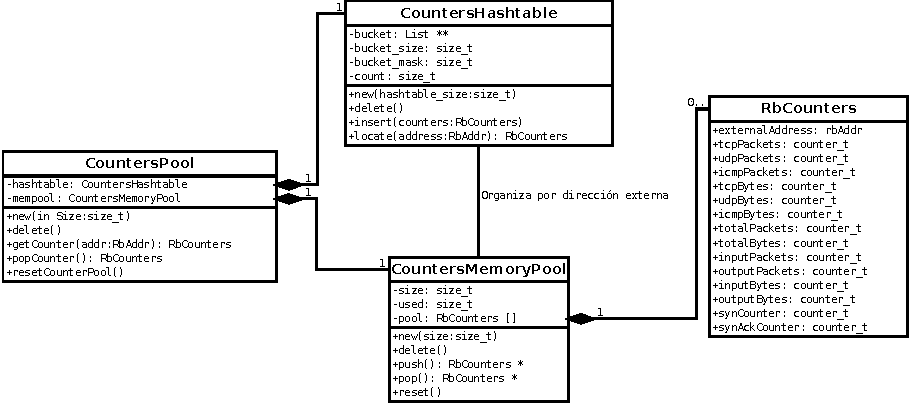
\includegraphics[width=\textwidth]{CapituloEstructura/Figuras/DiagramaClasesContadores-crop}
\caption{Diagrama de clases de la piscina de contadores}
\LABFIG{ClasesPoolContadores}
\end{figure}
%

A lo largo de la ejecución del programa, no se permitirá hacer nuevas reservas de memoria al \gls{SO} para 
nuevos contadores. En el caso de ataque, esto saturaría los recursos de los que dispone la máquina, por lo que tiene 
sentido ponerle un límite superior. Por otro lado, en caso de ataque repentino, no se debería perder tiempo en llamadas 
al \gls{SO} para pedir más memoria. Así pues, se dispondrá de un número limitado de contadores desde el inicio hasta el 
final de la ejecución del programa.

\subsubsection{Algoritmo del subcontador}
Tras ser enviado el paquete a una cola, le tocará ser procesado por un hilo contador. Cada hilo contador tiene 
asociadas dos piscinas de contadores\footnote{ver \SSSEC{Pool de contadores}.}. 

Cuando un nuevo paquete llega, la Función de Distribución\footnote{ver \SSEC{EstructuraCluster}.} lo habrá marcado como 
entrante o saliente, según la interfaz por la que ha entrado al Cluster. A partir de ahí, se extrae su \gls{IP} externa 
mediante el Algoritmo \ALG{ExtracciónIPExterna}.

\begin{algorithm}[htbp]
 \KwData{Paquete a analizar}
 \KwResult{Dirección del mismo }
 \eIf{paquete entrante}{
   ip externa $\gets$ ip origen\;
   }{
   ip externa $\gets$ ip destino\;
  }
 \caption{Algoritmo de extracción de IP externa}
 \LABALG{ExtracciónIPExterna}
\end{algorithm}

Tras ello, se pide a la piscina de contadores el contador asociado a la IP externa, y se actualiza la información 
pertinente, controlando siempre los errores como que la piscina esté llena y no pueda albergar ningún contador más.

En la \FIG{ActividadSubcontador} podemos ver el diagrama de actividad de esta función.

\begin{figure}[htbp]
\centering
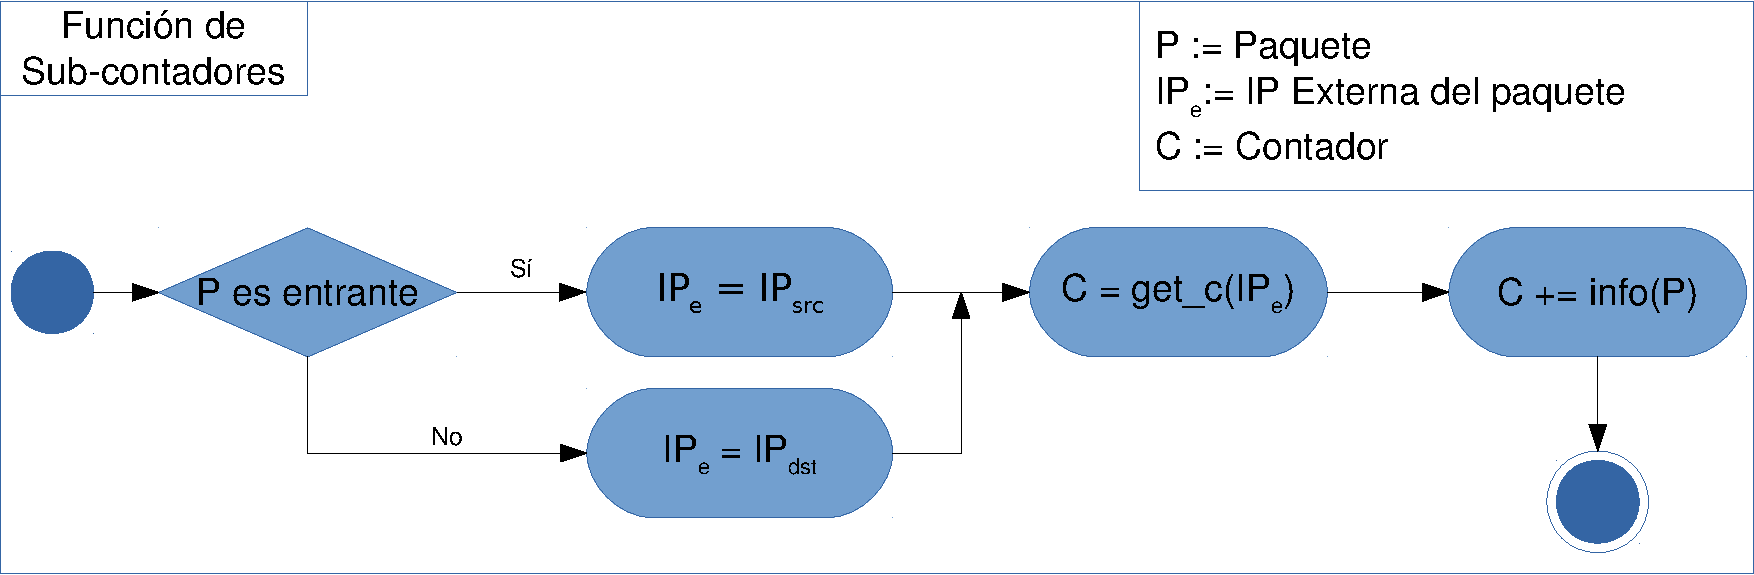
\includegraphics[width=\textwidth]{CapituloEstructura/Figuras/ActividadFuncionContador-crop}
\caption{Función de sub-contador}
\LABFIG{ActividadSubcontador}
\end{figure}
%

\subsection{Contador Maestro}\index{Contrador Maestro}
\subsubsection{Señal SIGALRM}\index{SIGALRM}
Para conseguir que la función del contador maestro se ejecute de una manera periódica, se usa la señal 
SIGALRM\index{Señales de GNU/Linux}\index{SIGALRM} de GNU/Linux (ver sección \SSEC{SIGALRM}). Cuando esta se produce, 
se activará una variable global \texttt{sigalrm\_received} y, si esta ya estaba activada en el momento que se produjo, 
se activará también \texttt{sigalrm\_accum}, como indicador de que \redborderddos{} no es capaz de procesar todo el 
flujo de tráfico.

\subsubsection{Mínima interrupción de los sub-contadores}
Los sub-contadores son la parte de \redborderddos que más carga de trabajo llevan. Es por eso por lo que se ha enfocado 
todo el diseño de la aplicación en hacerlos lo más escalable posible.

Sin embargo, es necesario recolectar los contadores y procesarlos en algún momento, con el fin de extraer los distintos 
estadísticos \gls{CUSUM}. Sería impensable bloquear los sub-contadores con el fin de extraer dichos estadísticos: Si la 
piscina está muy ocupada, la cola de paquetes se llenaría y nos veríamos obligados a tirar paquetes.

Para evitar detener los hilos sub-contadores un largo periodo de tiempo, se trabaja con punteros y con las variables 
cerrojo de la librería \gls{pthreads}\index{Librería pthread}. Cada hilo contador tiene reservados dos piscinas de 
contadores, y sólo usa en un periodo de tiempo una de ellas, que va llenando de contadores. Un puntero apunta al 
contador que está usando actualmente, situado en un vector que llamaremos \emph{Piscina Contadores}. Así, el contador 
que está usando el trabajador \emph{i} actualmente será \emph{Piscina contadores[i]}.

Cada hilo contador tiene asociado una variable cerrojo\index{Variable Cerrojo}, que bloquea cuando trabaja con su 
piscina. Cuando se activa la alarma del hilo principal, éste último bloquea dicha variable, e intercambia las piscinas 
de los hilos contadores, lo que se traduce en una simple asignación de punteros y esto, a su vez, se traduce como un 
tiempo mínimo de bloqueo.

Así pues, en el instante previo al lanzamiento de la alarma, el hilo contador ve una piscina llena de contadores, 
mientras que en el instante posterior ve una piscina nueva y limpia en la que almacenar. Para una descripción 
gráfica, ver \FIG{AntesSIGALRM} y \FIG{DespuesSIGALRM}.

\begin{figure}[htbp]
\centering
%\hfill
\subfloat[Instante antes de lanzar SIGALRM]%
   {\LABFIG{AntesSIGALRM}%
   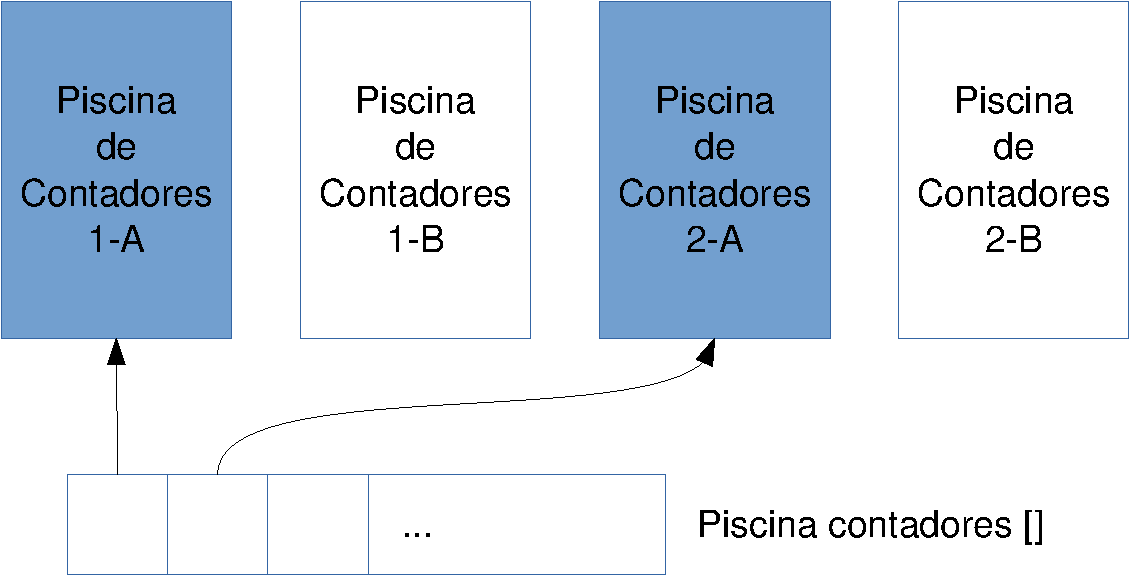
\includegraphics[width=0.45\textwidth]{CapituloEstructura/Figuras/DiagramaPoolsAntesSIGALRM-crop}}%
\hfill
\subfloat[Instante después de lanzar SIGALRM]%
 {\LABFIG{DespuesSIGALRM}%
 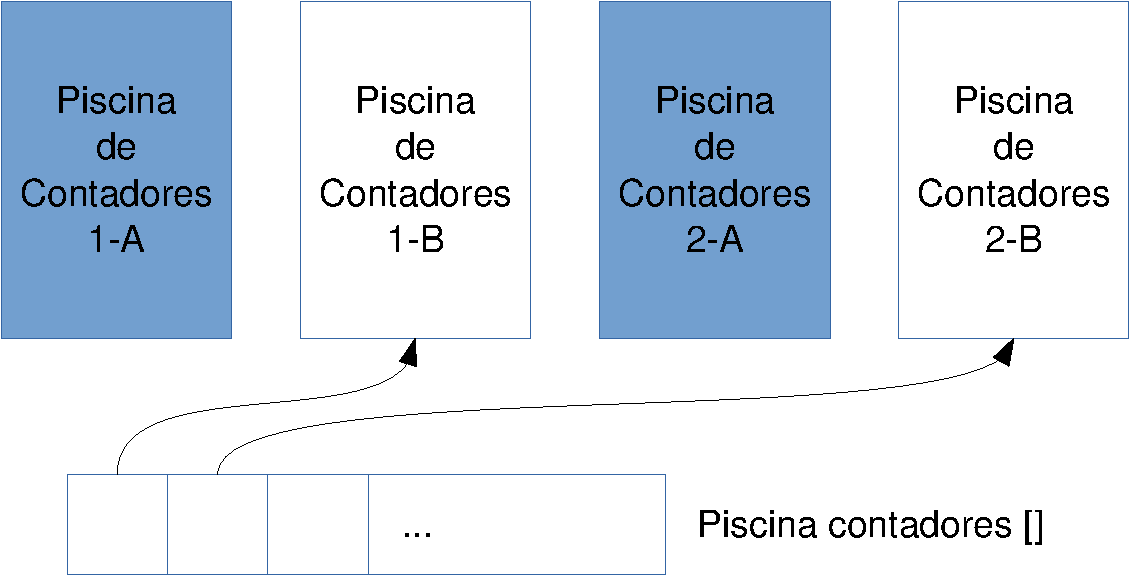
\includegraphics[width=0.45\textwidth]{CapituloEstructura/Figuras/DiagramaPoolsDespuesSIGALRM-crop}}%

\caption{Estado de las piscinas de contadores instantes antes y después de lanzar SIGALRM}
%\LABFIG{ActividadSubcontador}
\end{figure}
%

\subsubsection{Extración de estadísticos CUSUM}\LABSSSEC{ExtraccionEstadisticosCUSUM}

Tras intercambiar los contadores con el/los hilos contadores, el hilo maestro deberá extraer las estadísticas CUSUM de 
los mismos. Para ello, preparamos una estructura de datos con los parámetros de interés vistos en la 
\SSEC{Parametros de interés}. Por ello, de cada contador IP se debe extraer una muestra $x_i$ que indique el estado de 
las variables a controlar en ese momento.

Por comodidad, copiamos la estructura en \lstlistingname{} \ref{code:RbCusumStats}, y el algoritmo seguido para 
rellenarla en las ecuaciones desde \EQ{ExtractCusumTcpBytesRate} hasta \EQ{ExtractCusumInputOutputRate}.

\begin{align}
 \text{stats.tcp\_bytes\_percent}  &\gets \frac{\text{counters.tcp\_bytes   }}{\text{counters.total\_bytes}}
                                                                                    \LABEQ{ExtractCusumTcpBytesRate}\\
 \text{stats.udp\_bytes\_percent}  &\gets \frac{\text{counters.udp\_bytes   }}{\text{counters.total\_bytes}}\\
 \text{stats.icmp\_bytes\_percent} &\gets \frac{\text{counters.icmp\_bytes  }}{\text{counters.total\_bytes}}\\
%
 \text{stats.tcp\_pkts\_percent}   &\gets \frac{\text{counters.tcp\_pkts    }}{\text{counters.total\_pkts}}\\
 \text{stats.udp\_pkts\_percent}   &\gets \frac{\text{counters.udp\_pkts    }}{\text{counters.total\_pkts}}\\
 \text{stats.icmp\_pkts\_percent}  &\gets \frac{\text{counters.icmp\_pkts   }}{\text{counters.total\_pkts}}\\
%
 \text{stats.syn\_ack\_rate}       &\gets \frac{\text{counters.syn\_counter }}{\text{counters.ack\_counter}}\\
 \text{stats.input\_output\_prate} &\gets \frac{\text{counters.input\_pkts  }}{\text{counters.output\_pkts}}\\
 \text{stats.input\_output\_brate} &\gets \frac{\text{counters.input\_bytes }}{\text{counters.output\_bytes}}
                                                                                     \LABEQ{ExtractCusumInputOutputRate}
\end{align}

\begin{lstlisting}[language=C++,caption={Estructura estadísticos CUSUM}, breaklines=true, 
label=code:RbCusumStats,numbers=left,float=htbp]
typedef struct rb_cusum_stats_sample_s{
    double tcp_bytes_percent;   ///< TCP bytes/total bytes rate
    double udp_bytes_percent;   ///< UDP bytes/total bytes rate
    double icmp_bytes_percent;  ///< ICMP bytes/total bytes rate

    double tcp_pkts_percent;    ///< TCP paktes/total packets rate
    double udp_pkts_percent;    ///< UDP paktes/total packets rate
    double icmp_pkts_percent;   ///< ICMP paktes/total packets rate

    double syn_ack_rate;        ///< syn/ack rate

    double input_output_prate;   ///< Rate input/output packets
    double input_output_brate;   ///< Rate input/output bytes
}rb_cusum_stats_sample_t;
\end{lstlisting}

\subsubsection{Muestra completa de un estadístico CUSUM}
Como vimos en la \SEC{AlgoritmoCUSUM}, es necesario llevar el algoritmo CUSUM para el lado positivo y negativo ($C_i^+$ 
y $C_i^-$). Por tanto, con cada muestra debemos actualizar dos estadísticos \gls{CUSUM} por flujo o \gls{IP} externa.

Por ello, se debe crear una estructura que nos permita relacionar esas tres características. En cada ciclo del contador 
maestro, éste extraerá los contadores de los \texttt{CountersPool} vistos en \SSSEC{Pool de contadores} usando el 
método \texttt{popCounter} hasta que no haya más contadores (esto es, hasta que la misma devuelve \texttt{NULL}.

Por cada contador, extraemos una muestra $X_i$ como hemos visto en el \SSSEC{ExtraccionEstadisticosCUSUM}. Tras ello, 
aplicamos el algoritmo visto en la \SEC{AlgoritmoCUSUM}:

\begin{align}
 C_i^+ &= \max \left[0,\left\{C_{i-1}^+\left(x_i-\mu_0\right)\right\}-K\right] \\
 C_i^- &= \max \left[0,\left\{C_{i-1}^-\left(x_i-\mu_0\right)\right\}-K\right]
\end{align}

Donde $C_{i-1}$ es el contador almacenado en la anterior iteración.

No obstante, existe un problema con esta forma de actuar: es posible que en una iteración exista el $x_i$ de un 
contador, en la siguiente iteración no exista tráfico de esa dirección \gls{IP}, por lo que no se generaría ningún 
contador del mismo, y vuelva a existir el contador en la tercera iteración. De esa forma, si $T=-\mu_0-K$, $C_3$ 
quedaría:
\begin{align}
 C_3 = \max\left[0,C_1 + (x_3-T)\right] = \max\left[0,x_1-T+x_3-T\right] = 
       \max\left[0,x_1+x_3-2T\right] 
\end{align}
Sin embargo, al tener en cuenta $X_2=0$, $C_3$ debería quedar:
\begin{align}
 C_3 &= \max\left[0,C_1 + C_2 + (x_3-T)\right] = \max\left[0,x_1-T+0-T+x_3-T\right]
     =        \max\left[0,x_1 + x_3 -3T\right] 
\end{align}

Para salvar esa diferencia, tenemos dos opciones:
\begin{itemize}
 \item Escanear todo el espacio de direcciones CUSUM y actualizarlo.
 \item Almacenar, por cada CUSUM que se actualice, la marca de tiempo en la que fue actualizado.
\end{itemize}

Se elige, por razones de rendimiento, la segunda opción. Por tanto, la estructura para almacenar $C_i^+$ y $C_i^-$ 
quedan como se muestra en la \FIG{ClasesCusumSample}.

\begin{figure}[htbp]
\centering
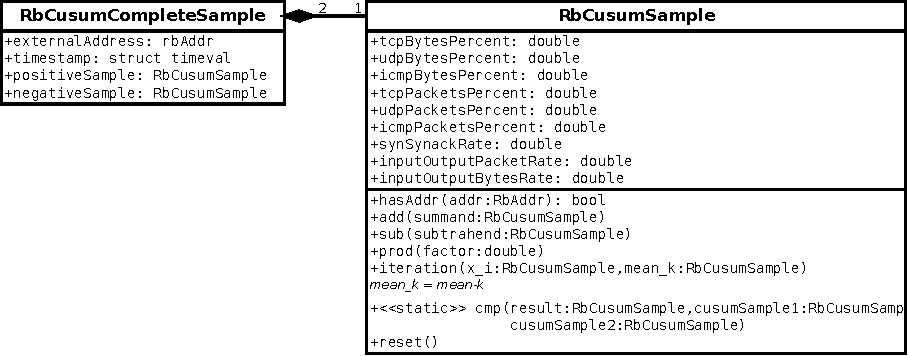
\includegraphics[width=\textwidth]{CapituloEstructura/Figuras/DiagramaClasesCusumSample-crop}
\caption{Diagrama de clases de las estructuras de almacenamiento de estadísticas CUSUM}
\LABFIG{ClasesCusumSample}
\end{figure}
%

Como funciones especiales que actúan sobre la estructura, se destacan \emph{iteration}, que realiza una iteración 
\gls{CUSUM} sobre la muestra, y \emph{cmp}, que guarda en una estructura del mismo tipo la comparación entre dos 
estructuras, aplicando el la comparación vista en Algoritmo\ALG{ComparacionFlotante} en cada miembro de la misma.

\subsubsection{Limpieza de estadísticos antiguos}\LABSSSEC{LimpiezaCusum}
Todo lo que se aprende, debe ser olvidado. Si pretendiésemos almacenar estadísticas \gls{CUSUM} por cada \gls{IP} que 
vemos indefinidamente, terminaríamos por saturar los contadores, y no podríamos seguir el comportamiento de ninguna 
dirección \gls{IP} más.

Por el momento, se reservará una cantidad fija de memoria para los estadísticos \gls{CUSUM}, y se almacenarán, a 
priori, en una lista de contadores \emph{libres}. A medida que se van necesitando, se almacenarán en otra lista de 
contadores \emph{en uso}. Es importante, desde el punto de vista del rendimiento, que la entrada de contadores en esta 
lista esté bien definida: O bien por la cabeza, o bien por la cola. A lo largo de este ejemplo, la entrada de 
estadísticos \gls{CUSUM} nuevos se realizará por la cabeza.

A intervalos de tiempo regulares, se realizará una limpieza de los contadores usados, comenzando por el lado inverso a 
la entrada de los mismos. En este ejemplo, el sentido elegido será la cola. Se elegirá un tiempo mínimo, a partir del 
cual, si el estadístico no ha sido actualizado tras esa marca de tiempo, será eliminado de la lista de 
estadísticos \emph{en uso} y pasará a la lista de \emph{libres}. Podemos ver este procedimiento en el 
Algoritmo\ALG{EliminacionContadoresAntigos} y en la \FIG{DiagramaActividadLimpiarLista}.

\begin{algorithm}
 \KwData{Lista de estadísticos cusum $l$, marca de tiempo $t$}
 \KwResult{Lista de estadísticos con sólo las entradas con marca de tiempo $t_0$ que cumplen $t_0>t$}
 \While{element $e \gets l.$last and $e.$timestamp $< t_0 $}{
	 usados.delete($e$)\;
	 libres.push($e$)\;
 }
 \caption{Procedimiento para la eliminación de contadores antiguos}
 \LABALG{EliminacionContadoresAntigos}
\end{algorithm}

\begin{figure}[htbp]
\centering
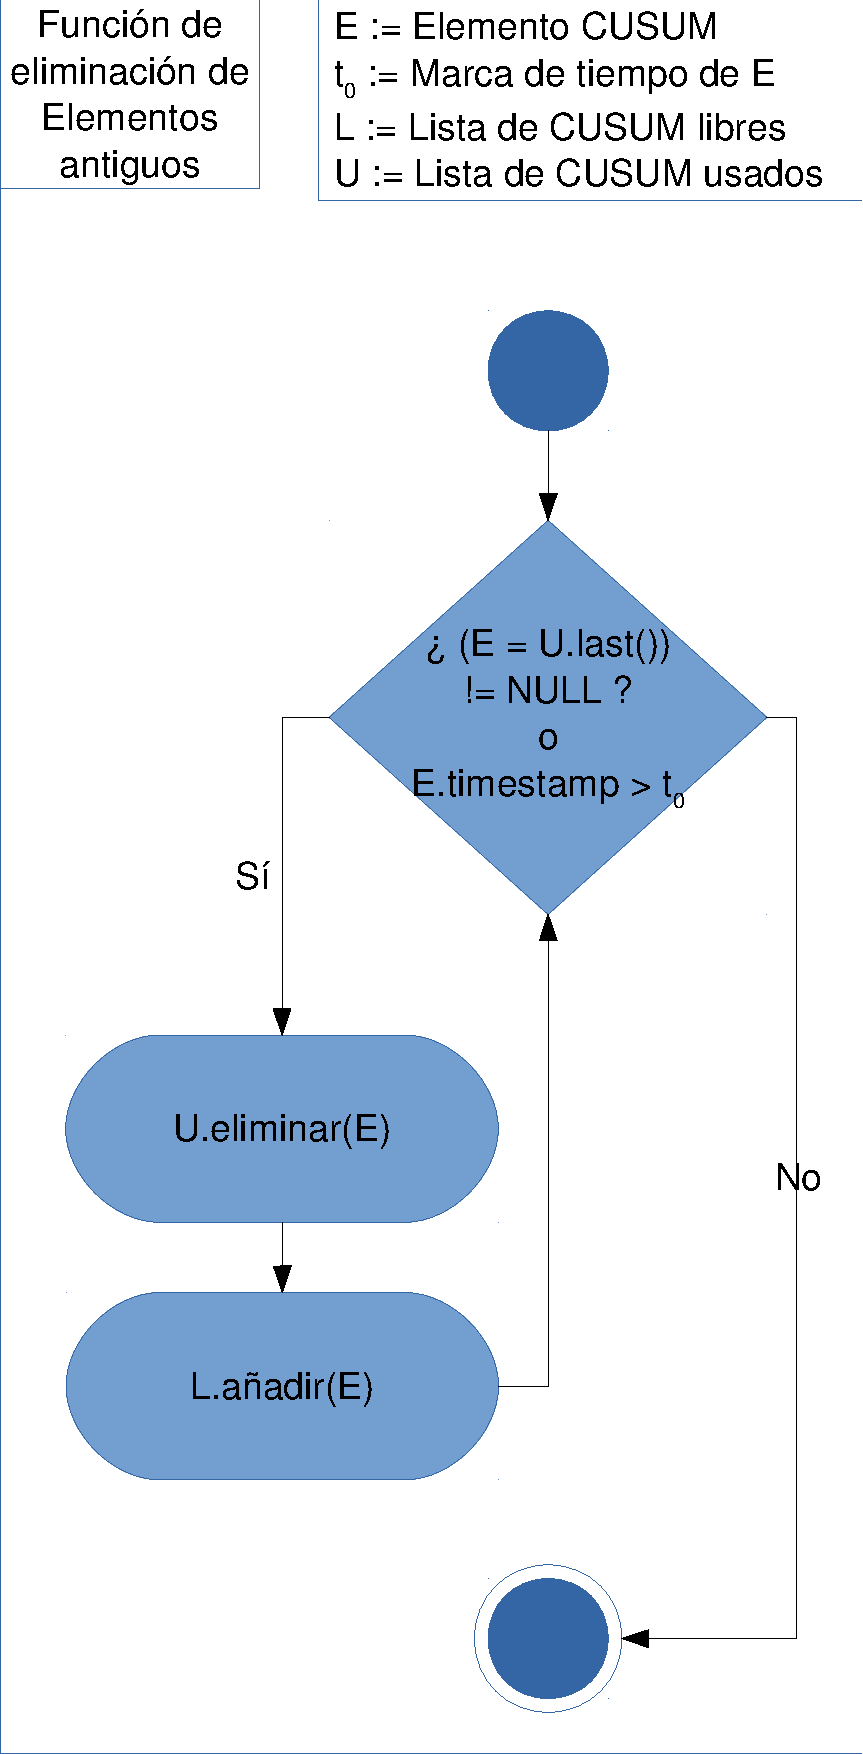
\includegraphics[width=0.4\textwidth]{CapituloEstructura/Figuras/ActividadFuncionLimpiarPoolCUSUM-crop}
\caption{Diagrama de actividad de la limpieza de estadísticos CUSUM antiguos}
\LABFIG{DiagramaActividadLimpiarLista}
\end{figure}
%

El orden de entrada y salida en la segunda lista no es relevante, si bien es preferible que esta actúe como una pila, 
con el fin de maximizar las probabilidades de que la memoria ocupada por los contadores se encuentre en la caché del 
procesador\footnote{Dicha caché eliminará las páginas que no han sido recientemente utilizadas. Si queremos volver a 
ellas, será necesario volver a recuperarlas de la RAM.}.

Cuando se use de nuevo un contador de la lista de contadores \emph{en uso}, esto es, se insertó en $C_i$ y se usó en 
$C_j j>i$, es necesario volver a colocarlo en la cabeza de la lista. Para ello, se deberá extraer de la misma, y volver 
a colocar en la cabeza. Si no se hiciese este paso, las marcas de tiempo de cada contador no estarían ordenadas en la 
lista, y la limpieza no sería efectiva.

Por ejemplo, si tenemos cinco flujos que están activos en un tiempo $t_i$, y nunca más vuelven a estar activos. Tras 
ellos, y sin haberse olvidado aún, llega un flujo en el instante $t_j j>i$ que, por ejemplo, se trata de un proceso 
automatizado que hace peticiones en un corto espacio de tiempo (por tanto, nunca olvidaremos ese flujo, ya que nunca 
será lo suficientemente antiguo).

Si no actualizamos la posición del elemento que ha llegado en $t_j$, y lo volvemos a colocar en la cabeza de la lista, 
nunca eliminaremos los elementos que llegaron antes.

\subsubsection{Pool de estadísticos CUSUM}

Al igual que ocurre con los contadores, el contador maestro necesita almacenar los diferentes estadísticos CUSUM que ha 
ido almacenando a lo largo del tiempo, y recuperarlos de una manera rápida. Para ello, se utiliza una estructura 
similar a la usada para almacenar y localizar los contadores: un Pool de estadísticos CUSUM.

Para ello, se utiliza una estructura similar a la vista en el \SSSEC{Pool de contadores}, pero necesita algunas 
diferencias. Mientras que la piscina de contadores tenía un ciclo de vida bien definido (nacía y moría en cada ciclo), 
esta estructura debe estar diseñada para vivir todo lo que viva el programa, por lo que necesita un método para 
eliminar entradas antiguas.

Por otro lado, no es necesario acceder, desde fuera de la misma, a los nodos almacenados de una manera 
lineal, es decir, como una lista.

\begin{figure}[htbp]
\centering
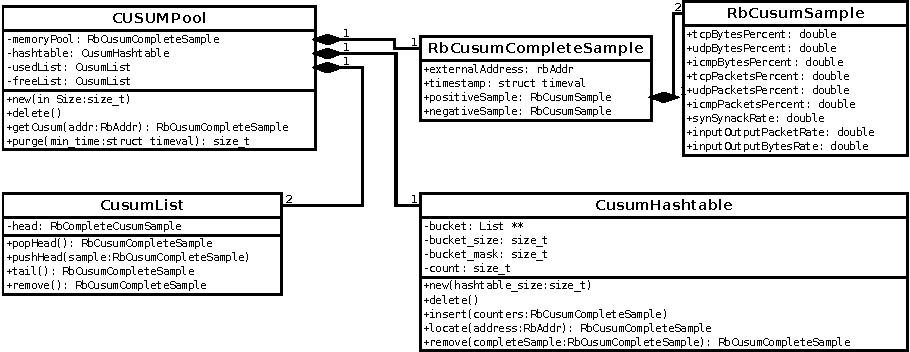
\includegraphics[width=\textwidth]{CapituloEstructura/Figuras/DiagramaClasesCUSUM-crop}
\caption{Diagrama de clases de la piscina de estadísticas CUSUM}
\LABFIG{ClasesCusumPool}
\end{figure}
%

Así pues, el diagrama de clases de la piscina de estadísticos \gls{CUSUM} se ve reflejado en \FIG{ClasesCusumPool}. 
Además del constructor y destructor, las funciones a destacar son \emph{getCusum}, que obtendrá la muestra completa 
\gls{CUSUM} que le indiquemos, y \emph{purge}, que eliminará de la piscina los contadores antiguos, siguiendo el 
algoritmo del \SSSEC{LimpiezaCusum}. Debido a ello, existen en la estructura las listas de estadísticos \emph{freeList} 
y \emph{usedList}.

En dichas listas podemos:
\begin{itemize}
 \item Añadir un elemento por la cabeza (inserción de un estadístico CUSUM).
 \item Eliminar un elemento por la cabeza (para extraer un elemento de la lista de libres).
 \item Acceder al elemento de la cola (para hacer la purga).
 \item Eliminar un elemento aleatorio de la lista.
\end{itemize}

Por último, para accesos aleatorios a los elementos tenemos la Tabla HASH, al igual que ocurría con la piscina de 
contadores. Es importante destacar que, al purgar los elementos, además de eliminarlos de la lista de elementos usados 
es necesario eliminarlos también de la tabla HASH. De otra forma, tendremos la entrada a un elemento eliminado.

\subsection{Decisor}\index{Decisor}
Periódicamente, el contador maestro recogerá.


\section{Resúmenes}%%%%%%%%%%%%%%%%%%%%%%%%%%%%%%%%%%%%%%%
\begin{Resumen}[Resumen de la estructura]
\subsection*{S1}
\end{Resumen}


%
% !TEX root =../LibroTipoETSI.tex
\chapter{Pruebas realizadas}\LABCHAP{EntornoPrueba}
\pagestyle{esitscCD}

\epigraph{What gets measured, gets managed.}{Peter Drucker}

\lettrine[lraise=-0.1, lines=2, loversize=0.25]{E}n este capítulo presentamos las pruebas realizadas al software con el 
fin de validar su comportamiento.

Se comenzará con las pruebas de laboratorio en la \SEC{PruebasLaboratorio}, destacando las más importantes para 
verificar el correcto funcionamiento de la aplicación, especialmente en el tema de falsos positivos 
(\SSEC{FalsosPositivos} y falsos negativos (\SSEC{FalsosNegativos}.

Para concluir, se pasará a una prueba más real y relevante realizada en Produban en la sección \SEC{PruebaProduban}

%TODO falta mas datos

\section{Pruebas de laboratorio}\LABSEC{PruebasLaboratorio}
\subsection{Entorno del laboratorio}

\begin{figure}[htbp]
\centering
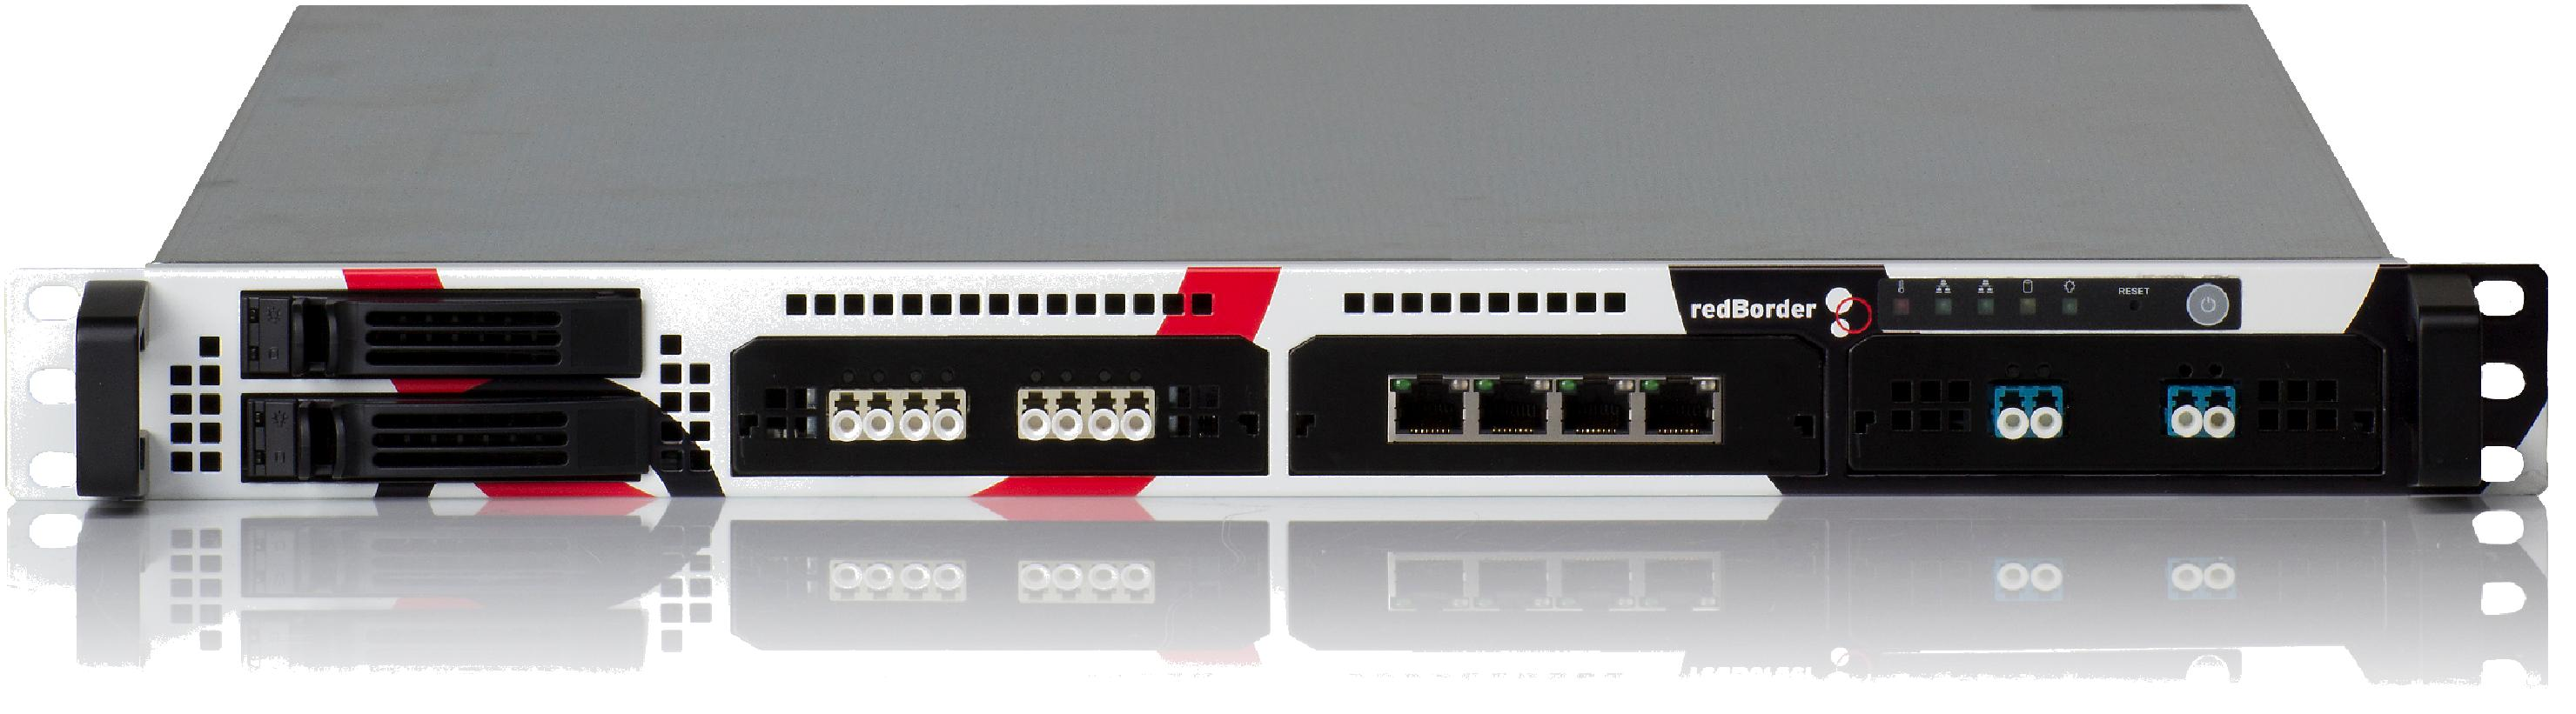
\includegraphics[width=\textwidth]{CapituloPruebas/Figuras/Sensor}
\caption{Device Under Test}
\LABFIG{DUT}
\end{figure}
%

El equipo \gls{DUT} es un redBorder IPS de 8 hilos (1 quad-core de 2 hilos por core) Intel Xeon E3-1240 a 3.30GHz. La 
interfaz del segmento de inspección es una intel quad-ethernet 82580 Gigabit con soporte bypass. En el sensor se ha 
instalado la distribución \emph{redBorder-IPS-sensor 3.0.30-1}, basada en la distribución Linux CentOS 6.5.

Como generador de tráfico, se usará otro dispositivo con las mismas características. Los segmentos de $1G$ se unirán de 
un equipo a otro en el mismo orden, a fin de facilitar el entendimiento de las pruebas, y serán llamados 
\text{eth4}, \text{eth5}, \text{eth6}, y \text{eth7} de izquierda a derecha.

En estos momentos, el controlador actual de la tarjeta de $10G$ no soporta $ZeroCopy$, por lo que habrá que hacer las 
pruebas en $1G$.

Se dispone, además de una captura de tráfico llamada \emph{entrenamiento.pcap}, que contiene tráfico real sin ataques.

\subsection{Prueba 1: Ajuste de los parámetros CUSUM para evitar falsos positivos}\LABSSEC{FalsosPositivos}
\subsubsection{Descripción de la prueba}
El primer paso de cara a realizar las pruebas es conseguir un valor adecuado de los parámetros $k$ y $h$. Como vimos en 
\CHAP{Algoritmo CUSUM}, el parámetro $k$ indica la magnitud que debe tener una muestra $x_i$ para que sume algo a 
$C_{i-1}$, en unidades de $\left[\sigma\right]$. El parámetro $h$, por su parte, indica el número de desviaciones 
típicas que debe alcanzar $C_i$ para que se deba lanzar una alerta.

Recordamos en \EQ{PruebasCusumPos} y \EQ{PruebasCusumNeg} las ecuaciones del algoritmo \gls{CUSUM}, por comodidad.
\begin{align}
 K &:= k\sigma \nonumber\\
 H &:= h\sigma \nonumber\\
 C_i^+ &= C_{i-1}^+ + (x_i-\mu_0-K) \LABEQ{PruebasCusumPos} \\
 C_i^+ &= C_{i-1}^+ - (x_i-\mu_0-K) \LABEQ{PruebasCusumNeg} \\
 &\text{Alarma si $C_i^\cdot > H$} \nonumber
\end{align}

\subsubsection{Procedimiento}
En procedimiento de la prueba será el siguiente:
\begin{enumerate}
 \item Se debe conocer la duración de la captura. 
 \item Se arranca el programa con un periodo de entrenamiento ligeramente inferior, ya que si la captura termina antes 
de tiempo, se registrarán muestras $0$ lo cual disminuirá la media. Por otro lado, si se repitiese, también disminuiría 
la desviación típica, lo que tampoco nos conviene.
 \item Tras el periodo de entrenamiento, se debe crear un fichero en \texttt{/var/log/ddos.log.<timestamp>} con los 
estadísticos registrados en ese periodo de tiempo.
 \item Se debe hacer pasar de nuevo la capruta por el sensor, pre-cargando los estadísticos con el parámetro 
\texttt{-l}, y con unos valores iniciales de $k$ y $h$. Se deben modificar a fin de encontrar unos valores que no 
generen alertas, ya que son claramente falsos positivos.
 \begin{enumerate}
  \item Si, tras un tiempo, existen varias direcciones \gls{IP} con un valor $C_i$ demasiado elevado, es porque $k$ 
estaba muy bajo.
  \item Si existen muchas alertas con valores $C_i$ bajos, es porque $h$ es demasiado bajo.
 \end{enumerate}
\end{enumerate}

Para lanzar la captura, se usó el comando tcpreplay, tras generar el archivo .cache:

\begin{verbatim}
[ @trafficgen pcap]$ tcpprep -i entrenamiento.pcap -o entrenamiento.cache
[ @trafficgen pcap]$ tcpreplay --cachefile entrenamiento.cache --intf1=eth4 --intf2=eth5
\end{verbatim}

Por su parte, \redborderddos fue lanzado con los siguientes parámetros en el entrenamiento:

\begin{verbatim}
[root@DUT rbddos]# ./rbddos -i eth4 -o eth7 -c 99 -r 0 -g 1:2:3:4:5:6  -m 7 -d -s 1024
\end{verbatim}

Y de esta otra manera en el periodo de defensa

\begin{verbatim}
[root@DUT rbddos]# ./rbddos -i eth4 -o eth7 -c 99 -r 0 -g 1:2:3:4:5:6  -m 7 -d -s 1024 -l /var/log/ddos.log.*
\end{verbatim}

Donde los parámetros usados significan:

\begin{verbatim}
 -i    Interfaz de entrada
 -o    Interfaz de salida
 -c    PF_RING cluster id
 -r    Núcleo usado para el balanceador
 -g    Núcleos usados para los contadores
 -m    Núcleo usado por el contador principal
 -d    Modo depuración
 -s    Tamaño de la piscina de contadores
 -l    Archivo de datos aprendidos
\end{verbatim}

Como valores iniciales, se escogieron los recomendados por Ismael Sánchez, $k=2.5$ y $h=5$ \cite{CUSUM_Carlos_III}.

\subsubsection{Resultados}
Tras realizar las pruebas, se observó que los valores negativos $C_i^-$ eran muy propensos a anunciar alarmas, deido 
a que el tráfico suele ser la mayor parte del tiempo $0$ y, durante un breve intervalo de tiempo, elevado. Por lo 
tanto, los distintos flujos están demasiado tiempo inactivos, lo que hace que se lance su alarma asociada.

% TODO
% Paquetes: 00, 01, 02, 03, 04, 05, 06, 07, 08, 09
% Total: 1528795 150000 ...
% ICMP: 15330 6614 5488 3651 5795 9547 4497 4939 4060 5440

Debido también a demasiadas alarmas, aquellas relacionadas con el protocolo \gls{ICMP} también tuvieron que ser 
desactivadas. La traza contenía muy pocos paquetes de este protocolo ($65361$ de $15000000$), por lo que se decidió 
descartar estas alarmas.

Finalmente, los parámetros para evitar falsas alarmas fueron ajustados a $k=5$ y $h=10$.

\subsection{Prueba 2: Detección de IPs atacantes, control de falsos negativos y estado de 
alerta}\LABSSEC{FalsosNegativos}
\subsubsection{Descripción de la prueba}
Para esta prueba, se necesitarán las cuatro interfaces de red. Con el aprendizaje de la prueba anterior, se hará pasar 
la captura \emph{entrenamiento.pcap} por uno de los dos segmentos, mientras que en el otro, al cabo de un tiempo $T_0$, 
se hará pasar tráfico claramente atacante: una ráfaga de paquetes UDP a alta velocidad, desde un pcap preparado.

Se modificará \texttt{rbddos} para que emita un mensaje si, en un ciclo, se ha visto bajo ataque, y para que emita el 
tráfico total visto. De esta forma, podremos saber si el programa funciona correctamente. Las IP normales estarán en 
una red distinta de las atacante (\texttt{172.26.0.0/16} frente a \texttt{10.0.0.0/8})

Se utilizarán los datos de entrenamiento de la anterior prueba.

\subsubsection{Procedimiento}
Se arranca el programa, ya en modo defensa por los datos aprendidos
\begin{verbatim}
[root@DUT rbddos]# ./rbddos -i eth4 -o eth7 -c 99 -r 0 -g 1:2:3:4:5:6  -m 7 -d -s 1024 -l /var/log/ddos.log.*
\end{verbatim}

Se hace pasar el tráfico por un segmento vía \texttt{tcpreplay}:
\begin{verbatim}
 tcpreplay --cachefile entrenamiento.cache --intf1=eth4 --intf2=eth5 entrenamiento.pcap
\end{verbatim}

Pasados 20 segundos, se hace pasar el tráfico UDP a alta velocidad por el otro segmento:
\begin{verbatim}
 tcpreplay -t --cachefile udp.cache --intf1=eth6 --intf2=eth7 udp.pcap
\end{verbatim}

Se detiene el pcap a los 10 segundos. Tras ello, se analiza la salida, y se registra, con la salida de depuración:
\begin{itemize}
 \item Número de paquetes analizados por el programa.
 \item Si el programa ha estado en alerta o no.
\end{itemize}

\subsubsection{Reultados}

\begin{figure}[htbp]
\centering
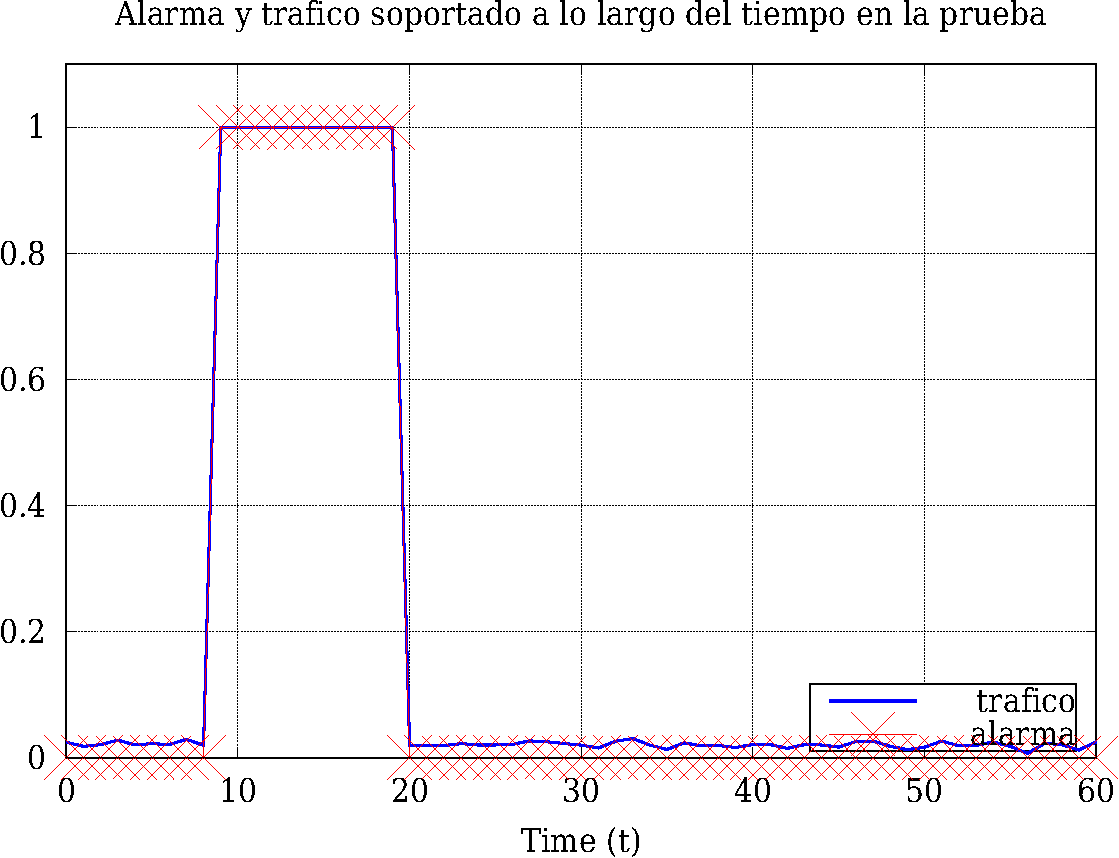
\includegraphics[width=\textwidth]{CapituloPruebas/Figuras/pruebaTrafico-crop}
\caption{Resultados de la prueba}
\LABFIG{PruebaTrafico}
\end{figure}
%

En los resultados, \texttt{rbddos} fue capaz de marcar los momentos ajo ataque a distintas velocidades, y todos los 
elementos atacantes pertenecían al conjunto de direcciones IP correctos.

\section{Prueba realizada en Produban}\LABSEC{PruebaProduban}
\subsection{Entorno}
El día 4 de mayo de 2013, Produbán, empresa de gestión IT del grupo Santanter, pidió a Eneo un sistema que de detección 
de ataques \gls{DDoS}, dado que tenía la sospecha de que se iba a producir un ataque real a su infraestructura.

Pese a estar aún en un estado muy prematuro, Produban aceptó la instalación del software ya que no entrañaba riesgo 
para la infraestructura al estar este situado en un puerto SPAN.

\begin{figure}[hbtp]
\centering
%\hfill
\subfloat[Frontal del sensor]%
   {\LABFIG{ProdubanFrontal}%
   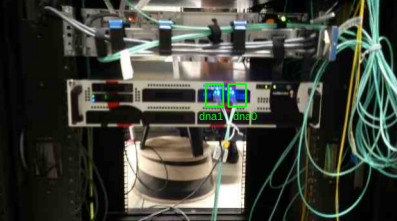
\includegraphics[width=0.49\textwidth]{CapituloPruebas/Figuras/ProdubanFrontal}}
\hfill
\subfloat[Parte trasera del sensor]%
   {\LABFIG{ProdubanTrasera}%
   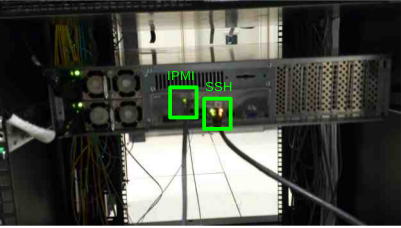
\includegraphics[width=0.49\textwidth]{CapituloPruebas/Figuras/ProdubanTrasera}}
%
\caption{Instalación de \redborderddos{} en el CPD de Mesena, Produban}
\end{figure}
%
El sensor usado es un equipo 2U con doble procesador Xeon E5 y 64GB de RAM, con 2 puertos dedicados de gestión y otros 
2 puertos 10G para conectarse a un puerto de SPAN, y es instalado en el CPD de Mesena.

En la \FIG{ProdubanFrontal} podemos ver la parte frontal del sensor, en la que fueron instalados dos pares de fibra 
óptica dirigidas a un puerto SPAN. Por otro lado, en la parte trasera, vemos la conexión de la interfaz de gestión y el 
puerto IPMI, una interfaz especial dirigida a manejar el sensor por web.

\subsection{Resultados}
Debido a lo inmediato de la instalación, fue imposible ajustar el sensor para que diese resultados significativos. Con 
sólo tres horas de entrenamiento, y sin ser estas siquiera determinantes, era muy difícil que la prueba diese 
resultados satisfactorios.

Los resultados fueron, en cuanto al periodo de aprendizaje:
\begin{table}[htbp]
 \centering
 \begin {tabular}{lll}
  Parámetro & Media & Desviación típica  \\\hline
  Paquetes TCP & 93\% & 0.02 \\
  Paquetes UDP & 5\%  & 0.02 \\
  Paquetes ICMP & 0 & 0      \\
  Relación I/O & 32,41 & 13,75 \\
  Longitud media del flujo & 593.54 & 59.57 \\
  Relación SYN/(SYN+ACK) & 593.54 & 59.57   
 \end {tabular}
\end{table}

Debido al estado altamente prematuro de la aplicación, el resultado de la relación SYN/(SYN+ACK) fue confiundido con el 
de la longitud media del flujo. Esto, junto con el escaso margen que tenían los valores ICMP, provocaron que el número 
de alarmas emitidas fuese enorme.

El programa estuvo ejecutándose desde el 7 de mayo a las 11:53\footnote{Timestamp: 1367920409} hasta el 15 de mayo a 
las 11:36, y se generaron más de 100 millones de alarmas.

Las conclusiones principales que se extrayeron fue que la realidad era mucho más cambiante de lo que permitía discernir 
tres horas de entrenamiento, o incluso un día, y que se debería de adaptar el protocolo CUSUM para hacer frente a esa 
realidad.

\section{Conclusiones}
Tras analizar las pruebas realizadas en este capítulo, se observa que el algoritmo CUSUM se enfrenta bien a las pruebas 
de laboratiorio, pero es incapaz, como lo hemos planteado, de hacer frente a una muestra variable como es el tráfico 
que enfrenta un sistema a lo largo del tiempo. Así pues, se deberán buscar o bien otros sistemas de control de 
procesos, o bien modificar el algoritmo CUSUM para lograr analizar correctamente dicha variablidad.


\endinput


%
% !TEX root =../LibroTipoETSI.tex
\chapter{Conclusiones}\LABCHAP{Conclusiones}
\pagestyle{esitscCD}

\lettrine[lraise=-0.1, lines=2, loversize=0.25]{T}ras haber investigado sobre la taxonomía de los distintos ataques 
\gls{DoS}, el método seguido para detectar parte de ellos, el uso de PF\_RING como acelerador de captura y las diversas 
pruebas realizadas, plasmamos en este capítulo las principales conclusiones.

\section{Taxonomía de los ataques DDoS}
Un ataque \gls{DDoS} es toda acción que impida el acceso de usuarios legítimos a un servicio. de información. Podemos 
dividirlos, según su método de detección, en dos grandes grupos: Ataques por inundación, que son aquellos destinados a 
saturar los recursos de algún elemento de la comunicación, y ataques semánticos, que buscan explotar algún fallo en el 
algoritmo de los procesos implicados en la comunicación.

Para detectar los primeros, se deben usar sistemas de descubrimiento de cambios en tráfico, esto es, se deben extraer 
las características \emph{normales} del tráfico, y analizar si el tráfico instantáneo entra dentro de esos parámetros o 
no.

Por otro lado, la forma idónea de detectar ataques semánticos es mediante la búsqueda de patrones. Esto es, se debe
analizar el contenido de los paquetes, y detectar de esa forma paquetes con contenido malicioso.

\section{Algoritmo CUSUM}
El algoritmo CUSUM es un sistema de control de procesos con memoria, esto es, un sistema de monitorización que permite 
detectar variaciones en la norma no solo basándose en el instante actual, sino en el comportamiento de la variable a lo 
largo del tiempo, sin requerir para ello almacenar todos sus estados anteriores.

De entre los posibles valores a monitorizar, se han escogido ocho valores que han demostrado ser representativos: 
Paquetes y bytes TCP, ICMP, UDP, densidad de conexiones de un solo sentido y relación entre paquetes entrantes y 
salientes.

Sin embargo, es necesario indicarle al algoritmo qué norma debe seguir el tráfico, y es la parte compleja de la 
situación. En las pruebas realizadas, el tráfico es sintético y predecible, pero el tráfico IP real varía mucho para un 
mismo segmento a diferentes horas del día, día de la semana, y periodos del año. Por ello, lo que se ha aprendido a una 
hora, no tiene por qué ser válido a la siguiente hora, y un tráfico legítimo puede ser clasificado rápidamente como 
ilegítimo. 

Así, CUSUM aplicado directamente no resulta una solución eficaz para la detección de anomalías en el tráfico de red y, 
por tanto, para detectar ataques \gls{DDoS}.

\section{PF\_RING y ZeroCopy}
PF\_RING es una tecnología diseñada para sustituir el tratamiento normal que el núcleo de Linux da a los paquetes 
destinados a la monitorización pasiva, eliminando redundancias y deficiencias que el modelo actual tiene. 

PF\_RING funciona, principalmente, reservando de antemano muchos de los recursos que la máquina necesita para almacenar 
un paquete, y evitando que éste pase por la pila normal del núcleo, la cual tiene el inconveniente de necesitar, 
fundamentalmente, excesivas copias de memoria y demasiadas llamadas al sistema.

Por su parte, ZeroCopy es un marco de trabajo en el que los paquetes se pueden distribuir entre aplicaciones sin 
necesitar por ello realizar varias copias para cada una de ellas. Si funcionamos en modo ZeroCopy puro, además, 
evitamos la copia de memoria entre la tarjeta, el núcleo y el espacio de usuario, consiguiendo así muchos más recursos 
para el procesado de paquetes, misión principal del sensor.

En las pruebas realizadas, ambas tecnologías se muestran muy beneficiosas a la hora de analizar el tráfico de manera 
pasiva, pasando de no ser capaz de superar los 7000mbps en un enlace saturado usando el 100\% de la CPU a leer a 
velocidad de cable usando sólo un 4\% de la CPU.

\endinput


% 
%%:Empezamos con los apéndices, que irían en uno o más ficheros. Es necesario incluir estos ficheros entre el entorno \begin{appendices}....\end{appendices} debido a que se ha deseado utilizar un formato diferente para el título de los apéndices, incluyendo la palabra apéndice, para la numeración de los apéndices, alfabético, y para las cabeceras de las páginas.
%
%\begin{appendices}
%
%% Fichero en el que se incluyen los apéndices
%% !TEX root =../LibroTipoETSI.tex

%APENDICE A
\chapter{Documentación de las estructuras}\LABAPEN{Doxygen}
A lo largo de este capítulo, repasamos la dosucmentación de las distintas estructuras usadas en la programación del 
proyecto

% Used for member lists
\newenvironment{DoxyCompactItemize}{%
  \begin{itemize}%
    \setlength{\itemsep}{-3pt}%
    \setlength{\parsep}{0pt}%
    \setlength{\topsep}{0pt}%
    \setlength{\partopsep}{0pt}%
}{%
  \end{itemize}%
}

\section{alarm\_data Struct Reference}
\label{structalarm__data}
\subsection*{Public Attributes}
\begin{DoxyCompactItemize}
\item 
time\_t {\bf timestamp}
\item 
double {\bf h}
\item 
const \\*
{\bf rb\_cusum\_stats\_complete\_sample\_t} $\ast$ {\bf threshold}
\item 
const \\*
{\bf rb\_cusum\_stats\_complete\_sample\_t} $\ast$ {\bf cmp}
\item 
const \\*
{\bf rb\_cusum\_stats\_complete\_sample\_t} $\ast$ {\bf stats}
\item 
{\bf rb\_string} $\ast$ {\bf alarm\_string}
\end{DoxyCompactItemize}


\subsection{Member Data Documentation}
\subsubsection[{alarm\_string}]{\setlength{\rightskip}{0pt plus 5cm}{\bf rb\_string}$\ast$ alarm\_data\+::alarm\_string}
String of the alarm. If new fields are added, it will be here.

\subsubsection[{cmp}]{\setlength{\rightskip}{0pt plus 5cm}const {\bf rb\_cusum\_stats\_complete\_sample\_t}$\ast$ alarm\_data\+::cmp}
Result of stats-threshold comparison

\subsubsection[{h}]{\setlength{\rightskip}{0pt plus 5cm}double alarm\_data\+::h}
Current CUSUM h

\subsubsection[{stats}]{\setlength{\rightskip}{0pt plus 5cm}const {\bf rb\_cusum\_stats\_complete\_sample\_t}$\ast$ alarm\_data\+::stats}
Current $C_i$

\subsubsection[{threshold}]{\setlength{\rightskip}{0pt plus 5cm}const {\bf rb\_cusum\_stats\_complete\_sample\_t}$\ast$ alarm\_data\+::threshold}
Current threshold

\subsubsection[{timestamp}]{\setlength{\rightskip}{0pt plus 5cm}time\_t alarm\_data\+::timestamp}
Current timestamp


The documentation for this struct was generated from the following file\+:\begin{DoxyCompactItemize}
\item 
{\bf rb\_cusum\_ddos.\+c}\end{DoxyCompactItemize}

\section{packet\_info\_s Struct Reference}
\label{structpacket__info__s}\index{packet\_info\_s@{packet\_info\_s}}


Struct to store all packet information needed.  


\subsection*{Public Attributes}
\begin{DoxyCompactItemize}
\item 
{\bf rb\_counters\_t} $\ast$ {\bf global\_counters}
\begin{DoxyCompactList}\small\item\em Global counters. \end{DoxyCompactList}\item 
{\bf rb\_counters\_t} $\ast$ {\bf counters}
\begin{DoxyCompactList}\small\item\em Flow counters. \end{DoxyCompactList}\item 
size\_t {\bf packet\_len}
\begin{DoxyCompactList}\small\item\em Packet len at level 2. \end{DoxyCompactList}\item 
{\bf direction\_t} {\bf direction}
\begin{DoxyCompactList}\small\item\em Packet direction. \end{DoxyCompactList}\end{DoxyCompactItemize}


\subsection{Detailed Description}
Struct to store all packet information needed. 

\subsection{Member Data Documentation}
\index{packet\_info\_s@{packet\_info\_s}!counters@{counters}}
\index{counters@{counters}!packet\_info\_s@{packet\_info\_s}}
\subsubsection[{counters}]{\setlength{\rightskip}{0pt plus 5cm}{\bf rb\_counters\_t}$\ast$ packet\_info\_s\+::counters}\label{structpacket__info__s_af735e249b83dc2855bad3eb823c770be}


Flow counters. 

\index{packet\_info\_s@{packet\_info\_s}!direction@{direction}}
\index{direction@{direction}!packet\_info\_s@{packet\_info\_s}}
\subsubsection[{direction}]{\setlength{\rightskip}{0pt plus 5cm}{\bf direction\_t} packet\_info\_s\+::direction}\label{structpacket__info__s_ac8ab4e7c00ec07b9444c7a52f83eb892}


Packet direction. 

\index{packet\_info\_s@{packet\_info\_s}!global\_counters@{global\_counters}}
\index{global\_counters@{global\_counters}!packet\_info\_s@{packet\_info\_s}}
\subsubsection[{global\_counters}]{\setlength{\rightskip}{0pt plus 5cm}{\bf rb\_counters\_t}$\ast$ packet\_info\_s\+::global\_counters}\label{structpacket__info__s_a4d1609e7554b71ba9f97e973aee535ee}


Global counters. 

\index{packet\_info\_s@{packet\_info\_s}!packet\_len@{packet\_len}}
\index{packet\_len@{packet\_len}!packet\_info\_s@{packet\_info\_s}}
\subsubsection[{packet\_len}]{\setlength{\rightskip}{0pt plus 5cm}size\_t packet\_info\_s\+::packet\_len}\label{structpacket__info__s_a1f6f94ed26fa196c221624ee9a2a7c6a}


Packet len at level 2. 



The documentation for this struct was generated from the following file\+:\begin{DoxyCompactItemize}
\item 
{\bf engine.\+c}\end{DoxyCompactItemize}

\section{pfring\+\_\+zc\+\_\+pkt\+\_\+buff\+\_\+meta\+\_\+s Struct Reference}
\label{structpfring__zc__pkt__buff__meta__s}\index{pfring\+\_\+zc\+\_\+pkt\+\_\+buff\+\_\+meta\+\_\+s@{pfring\+\_\+zc\+\_\+pkt\+\_\+buff\+\_\+meta\+\_\+s}}


{\ttfamily \#include $<$engine.\+h$>$}

\subsection*{Public Attributes}
\begin{DoxyCompactItemize}
\item 
{\bf direction\+\_\+t} {\bf direction}
\begin{DoxyCompactList}\small\item\em Packet direction. \end{DoxyCompactList}\end{DoxyCompactItemize}


\subsection{Detailed Description}
pfring\+\_\+zc\+\_\+pkt\+\_\+buff user metadata 

\subsection{Member Data Documentation}
\index{pfring\+\_\+zc\+\_\+pkt\+\_\+buff\+\_\+meta\+\_\+s@{pfring\+\_\+zc\+\_\+pkt\+\_\+buff\+\_\+meta\+\_\+s}!direction@{direction}}
\index{direction@{direction}!pfring\+\_\+zc\+\_\+pkt\+\_\+buff\+\_\+meta\+\_\+s@{pfring\+\_\+zc\+\_\+pkt\+\_\+buff\+\_\+meta\+\_\+s}}
\subsubsection[{direction}]{\setlength{\rightskip}{0pt plus 5cm}{\bf direction\+\_\+t} pfring\+\_\+zc\+\_\+pkt\+\_\+buff\+\_\+meta\+\_\+s\+::direction}\label{structpfring__zc__pkt__buff__meta__s_a1ecea60e20e8ee0ff0fff4834e013a11}


Packet direction. 



The documentation for this struct was generated from the following file\+:\begin{DoxyCompactItemize}
\item 
{\bf engine.\+h}\end{DoxyCompactItemize}

\section{rb\_addr\_s Struct Reference}
\label{structrb__addr__s}\index{rb\_addr\_s@{rb\_addr\_s}}


Abstraction for ipv4 and v6 address.  




{\ttfamily \#include $<$rb\_addr.\+h$>$}

\subsection*{Public Attributes}
\begin{DoxyCompactItemize}
\item 
uint8\_t {\bf addr\_family}
\begin{DoxyCompactList}\small\item\em Family of address\+: A\+F\_\+I\+N\+E\+T or A\+F\_\+I\+N\+E\+T6. \end{DoxyCompactList}\item 
\begin{tabbing}
xx\=xx\=xx\=xx\=xx\=xx\=xx\=xx\=xx\=\kill
union \{\\
\>struct in\_addr {\bf sin\_addr}\\
\>struct in6\_addr {\bf sin6\_addr}\\
\} {\bf addr}\\

\end{tabbing}\begin{DoxyCompactList}\small\item\em Real buffer storing the address. \end{DoxyCompactList}\end{DoxyCompactItemize}


\subsection{Detailed Description}
Abstraction for ipv4 and v6 address. 

\subsection{Member Data Documentation}
\index{rb\_addr\_s@{rb\_addr\_s}!addr@{addr}}
\index{addr@{addr}!rb\_addr\_s@{rb\_addr\_s}}
\subsubsection[{addr}]{\setlength{\rightskip}{0pt plus 5cm}union \{ ... \}  rb\_addr\_s\+::addr}\label{structrb__addr__s_ab669e4f43ac662476dd7e1824f28f422}


Real buffer storing the address. 

\index{rb\_addr\_s@{rb\_addr\_s}!addr\_family@{addr\_family}}
\index{addr\_family@{addr\_family}!rb\_addr\_s@{rb\_addr\_s}}
\subsubsection[{addr\_family}]{\setlength{\rightskip}{0pt plus 5cm}uint8\_t rb\_addr\_s\+::addr\_family}\label{structrb__addr__s_a0eab82f9cdc545c452068f24a8f64cc1}


Family of address\+: A\+F\_\+I\+N\+E\+T or A\+F\_\+I\+N\+E\+T6. 

\index{rb\_addr\_s@{rb\_addr\_s}!sin6\_addr@{sin6\_addr}}
\index{sin6\_addr@{sin6\_addr}!rb\_addr\_s@{rb\_addr\_s}}
\subsubsection[{sin6\_addr}]{\setlength{\rightskip}{0pt plus 5cm}struct in6\_addr rb\_addr\_s\+::sin6\_addr}\label{structrb__addr__s_a272dcafb5295c1f8d999f860a96b2fd5}
\index{rb\_addr\_s@{rb\_addr\_s}!sin\_addr@{sin\_addr}}
\index{sin\_addr@{sin\_addr}!rb\_addr\_s@{rb\_addr\_s}}
\subsubsection[{sin\_addr}]{\setlength{\rightskip}{0pt plus 5cm}struct in\_addr rb\_addr\_s\+::sin\_addr}\label{structrb__addr__s_ac26433c8034f129ed3f06f44e63df305}


The documentation for this struct was generated from the following file\+:\begin{DoxyCompactItemize}
\item 
{\bf rb\_addr.\+h}\end{DoxyCompactItemize}

\section{rb\_counters\_memory\_pool\_s Struct Reference}
\label{structrb__counters__memory__pool__s}\index{rb\_counters\_memory\_pool\_s@{rb\_counters\_memory\_pool\_s}}


{\ttfamily \#include $<$rb\_counters\_memory\_pool.\+h$>$}

\subsection*{Public Attributes}
\begin{DoxyCompactItemize}
\item 
size\_t {\bf size}
\begin{DoxyCompactList}\small\item\em Pool size, [elements] unit. \end{DoxyCompactList}\item 
size\_t {\bf used}
\begin{DoxyCompactList}\small\item\em Elements used in the pool. \end{DoxyCompactList}\item 
int {\bf flags}
\begin{DoxyCompactList}\small\item\em Flags relative to the buffer. \end{DoxyCompactList}\item 
{\bf rb\_counters\_t} $\ast$ {\bf pool}
\begin{DoxyCompactList}\small\item\em Real pool buffer. \end{DoxyCompactList}\end{DoxyCompactItemize}


\subsection{Detailed Description}
Pool type. \begin{DoxyNote}{Note}
Never use directly. Use auxiliar functions. 
\end{DoxyNote}


\subsection{Member Data Documentation}
\index{rb\_counters\_memory\_pool\_s@{rb\_counters\_memory\_pool\_s}!flags@{flags}}
\index{flags@{flags}!rb\_counters\_memory\_pool\_s@{rb\_counters\_memory\_pool\_s}}
\subsubsection[{flags}]{\setlength{\rightskip}{0pt plus 5cm}int rb\_counters\_memory\_pool\_s\+::flags}\label{structrb__counters__memory__pool__s_afb2ebc67257a860c5e19bc33a7735b32}


Flags relative to the buffer. 

\index{rb\_counters\_memory\_pool\_s@{rb\_counters\_memory\_pool\_s}!pool@{pool}}
\index{pool@{pool}!rb\_counters\_memory\_pool\_s@{rb\_counters\_memory\_pool\_s}}
\subsubsection[{pool}]{\setlength{\rightskip}{0pt plus 5cm}{\bf rb\_counters\_t}$\ast$ rb\_counters\_memory\_pool\_s\+::pool}\label{structrb__counters__memory__pool__s_a35c4d7d5ab4718a7841cbcffb3a23bc3}


Real pool buffer. 

\index{rb\_counters\_memory\_pool\_s@{rb\_counters\_memory\_pool\_s}!size@{size}}
\index{size@{size}!rb\_counters\_memory\_pool\_s@{rb\_counters\_memory\_pool\_s}}
\subsubsection[{size}]{\setlength{\rightskip}{0pt plus 5cm}size\_t rb\_counters\_memory\_pool\_s\+::size}\label{structrb__counters__memory__pool__s_a884d46240b78bb76ae0969006b3ff5df}


Pool size, [elements] unit. 

\index{rb\_counters\_memory\_pool\_s@{rb\_counters\_memory\_pool\_s}!used@{used}}
\index{used@{used}!rb\_counters\_memory\_pool\_s@{rb\_counters\_memory\_pool\_s}}
\subsubsection[{used}]{\setlength{\rightskip}{0pt plus 5cm}size\_t rb\_counters\_memory\_pool\_s\+::used}\label{structrb__counters__memory__pool__s_a52376ec30e09f9131677466d599433fe}


Elements used in the pool. 



The documentation for this struct was generated from the following file\+:\begin{DoxyCompactItemize}
\item 
{\bf rb\_counters\_memory\_pool.\+h}\end{DoxyCompactItemize}

\section{rb\+\_\+counters\+\_\+pool Struct Reference}
\label{structrb__counters__pool}\index{rb\+\_\+counters\+\_\+pool@{rb\+\_\+counters\+\_\+pool}}


Pool of counters, that include tools for allocate and search counters.  


\subsection*{Public Attributes}
\begin{DoxyCompactItemize}
\item 
{\bf rb\+\_\+counters\+\_\+hashtable\+\_\+t} {\bf hashtable}
\begin{DoxyCompactList}\small\item\em Hashtable. \end{DoxyCompactList}\item 
size\+\_\+t {\bf hashtable\+\_\+size}
\item 
{\bf rb\+\_\+counters\+\_\+memory\+\_\+pool\+\_\+t} {\bf mempool}
\begin{DoxyCompactList}\small\item\em Real counters pool. Memory segment where will be stored. \end{DoxyCompactList}\end{DoxyCompactItemize}


\subsection{Detailed Description}
Pool of counters, that include tools for allocate and search counters. 

\subsection{Member Data Documentation}
\index{rb\+\_\+counters\+\_\+pool@{rb\+\_\+counters\+\_\+pool}!hashtable@{hashtable}}
\index{hashtable@{hashtable}!rb\+\_\+counters\+\_\+pool@{rb\+\_\+counters\+\_\+pool}}
\subsubsection[{hashtable}]{\setlength{\rightskip}{0pt plus 5cm}{\bf rb\+\_\+counters\+\_\+hashtable\+\_\+t} rb\+\_\+counters\+\_\+pool\+::hashtable}\label{structrb__counters__pool_adf9ebd540d7dfff78c737ea2347a39ed}


Hashtable. 

\index{rb\+\_\+counters\+\_\+pool@{rb\+\_\+counters\+\_\+pool}!hashtable\+\_\+size@{hashtable\+\_\+size}}
\index{hashtable\+\_\+size@{hashtable\+\_\+size}!rb\+\_\+counters\+\_\+pool@{rb\+\_\+counters\+\_\+pool}}
\subsubsection[{hashtable\+\_\+size}]{\setlength{\rightskip}{0pt plus 5cm}size\+\_\+t rb\+\_\+counters\+\_\+pool\+::hashtable\+\_\+size}\label{structrb__counters__pool_a1516ccdced571000d2faf01ff537ddf3}
\index{rb\+\_\+counters\+\_\+pool@{rb\+\_\+counters\+\_\+pool}!mempool@{mempool}}
\index{mempool@{mempool}!rb\+\_\+counters\+\_\+pool@{rb\+\_\+counters\+\_\+pool}}
\subsubsection[{mempool}]{\setlength{\rightskip}{0pt plus 5cm}{\bf rb\+\_\+counters\+\_\+memory\+\_\+pool\+\_\+t} rb\+\_\+counters\+\_\+pool\+::mempool}\label{structrb__counters__pool_ad42bea24eec7e2c7ea42865b0777f5ca}


Real counters pool. Memory segment where will be stored. 



The documentation for this struct was generated from the following file\+:\begin{DoxyCompactItemize}
\item 
{\bf rb\+\_\+counters\+\_\+pool.\+c}\end{DoxyCompactItemize}

\section{rb\+\_\+counters\+\_\+s Struct Reference}
\label{structrb__counters__s}\index{rb\+\_\+counters\+\_\+s@{rb\+\_\+counters\+\_\+s}}


{\ttfamily \#include $<$rb\+\_\+counters.\+h$>$}

\subsection*{Public Attributes}
\begin{DoxyCompactItemize}
\item 
uint64\+\_\+t {\bf magic}
\begin{DoxyCompactList}\small\item\em Just useful for integrity. \end{DoxyCompactList}\item 
{\bf rb\+\_\+addr\+\_\+t} {\bf external\+\_\+address}
\begin{DoxyCompactList}\small\item\em External I\+P address. \end{DoxyCompactList}\item 
uint32\+\_\+t {\bf tcp\+\_\+pkts}
\begin{DoxyCompactList}\small\item\em number tcp packets in the flow \end{DoxyCompactList}\item 
uint32\+\_\+t {\bf udp\+\_\+pkts}
\begin{DoxyCompactList}\small\item\em number udp packets in the flow \end{DoxyCompactList}\item 
uint32\+\_\+t {\bf icmp\+\_\+pkts}
\begin{DoxyCompactList}\small\item\em number icmp packets in the flow \end{DoxyCompactList}\item 
uint32\+\_\+t {\bf total\+\_\+pkts}
\begin{DoxyCompactList}\small\item\em total number packets in the flow \end{DoxyCompactList}\item 
uint32\+\_\+t {\bf tcp\+\_\+bytes}
\begin{DoxyCompactList}\small\item\em tcp bytes in the flow \end{DoxyCompactList}\item 
uint32\+\_\+t {\bf udp\+\_\+bytes}
\begin{DoxyCompactList}\small\item\em udp bytes in the flow \end{DoxyCompactList}\item 
uint32\+\_\+t {\bf icmp\+\_\+bytes}
\begin{DoxyCompactList}\small\item\em icmp bytes in the flow \end{DoxyCompactList}\item 
uint32\+\_\+t {\bf total\+\_\+bytes}
\begin{DoxyCompactList}\small\item\em total bytes in the flow \end{DoxyCompactList}\item 
uint32\+\_\+t {\bf input\+\_\+pkts}
\begin{DoxyCompactList}\small\item\em Input packets in the flow;. \end{DoxyCompactList}\item 
uint32\+\_\+t {\bf output\+\_\+pkts}
\begin{DoxyCompactList}\small\item\em Output packets in the flow;. \end{DoxyCompactList}\item 
uint32\+\_\+t {\bf input\+\_\+bytes}
\begin{DoxyCompactList}\small\item\em Input bytes in the flow;. \end{DoxyCompactList}\item 
uint32\+\_\+t {\bf output\+\_\+bytes}
\begin{DoxyCompactList}\small\item\em Output bytes in the flow;. \end{DoxyCompactList}\item 
uint32\+\_\+t {\bf syn\+\_\+counter}
\begin{DoxyCompactList}\small\item\em Number of tcp packets with syn flag enabled. \end{DoxyCompactList}\item 
uint32\+\_\+t {\bf ack\+\_\+counter}
\begin{DoxyCompactList}\small\item\em Number of tcp packets with ack flag enabled. \end{DoxyCompactList}\item 
tommy\+\_\+hashtable\+\_\+node {\bf hashtable\+\_\+node}
\begin{DoxyCompactList}\small\item\em Node iterator to store and recover for hashtable node. \end{DoxyCompactList}\end{DoxyCompactItemize}


\subsection{Detailed Description}
Fundamental counters structure 

\subsection{Member Data Documentation}
\index{rb\+\_\+counters\+\_\+s@{rb\+\_\+counters\+\_\+s}!ack\+\_\+counter@{ack\+\_\+counter}}
\index{ack\+\_\+counter@{ack\+\_\+counter}!rb\+\_\+counters\+\_\+s@{rb\+\_\+counters\+\_\+s}}
\subsubsection[{ack\+\_\+counter}]{\setlength{\rightskip}{0pt plus 5cm}uint32\+\_\+t rb\+\_\+counters\+\_\+s\+::ack\+\_\+counter}\label{structrb__counters__s_ad56857cdaf1a1d6f0e48369370452555}


Number of tcp packets with ack flag enabled. 

\index{rb\+\_\+counters\+\_\+s@{rb\+\_\+counters\+\_\+s}!external\+\_\+address@{external\+\_\+address}}
\index{external\+\_\+address@{external\+\_\+address}!rb\+\_\+counters\+\_\+s@{rb\+\_\+counters\+\_\+s}}
\subsubsection[{external\+\_\+address}]{\setlength{\rightskip}{0pt plus 5cm}{\bf rb\+\_\+addr\+\_\+t} rb\+\_\+counters\+\_\+s\+::external\+\_\+address}\label{structrb__counters__s_a0c78d881462006b548458e6c3b203fce}


External I\+P address. 

\index{rb\+\_\+counters\+\_\+s@{rb\+\_\+counters\+\_\+s}!hashtable\+\_\+node@{hashtable\+\_\+node}}
\index{hashtable\+\_\+node@{hashtable\+\_\+node}!rb\+\_\+counters\+\_\+s@{rb\+\_\+counters\+\_\+s}}
\subsubsection[{hashtable\+\_\+node}]{\setlength{\rightskip}{0pt plus 5cm}tommy\+\_\+hashtable\+\_\+node rb\+\_\+counters\+\_\+s\+::hashtable\+\_\+node}\label{structrb__counters__s_ae3969735e584c9d4b3ad8177cd37a43c}


Node iterator to store and recover for hashtable node. 

\index{rb\+\_\+counters\+\_\+s@{rb\+\_\+counters\+\_\+s}!icmp\+\_\+bytes@{icmp\+\_\+bytes}}
\index{icmp\+\_\+bytes@{icmp\+\_\+bytes}!rb\+\_\+counters\+\_\+s@{rb\+\_\+counters\+\_\+s}}
\subsubsection[{icmp\+\_\+bytes}]{\setlength{\rightskip}{0pt plus 5cm}uint32\+\_\+t rb\+\_\+counters\+\_\+s\+::icmp\+\_\+bytes}\label{structrb__counters__s_aa06f1ab9ee525c6559ee80637013f92d}


icmp bytes in the flow 

\index{rb\+\_\+counters\+\_\+s@{rb\+\_\+counters\+\_\+s}!icmp\+\_\+pkts@{icmp\+\_\+pkts}}
\index{icmp\+\_\+pkts@{icmp\+\_\+pkts}!rb\+\_\+counters\+\_\+s@{rb\+\_\+counters\+\_\+s}}
\subsubsection[{icmp\+\_\+pkts}]{\setlength{\rightskip}{0pt plus 5cm}uint32\+\_\+t rb\+\_\+counters\+\_\+s\+::icmp\+\_\+pkts}\label{structrb__counters__s_a6d5c2ba252a0952f600eccfa2d8bde17}


number icmp packets in the flow 

\index{rb\+\_\+counters\+\_\+s@{rb\+\_\+counters\+\_\+s}!input\+\_\+bytes@{input\+\_\+bytes}}
\index{input\+\_\+bytes@{input\+\_\+bytes}!rb\+\_\+counters\+\_\+s@{rb\+\_\+counters\+\_\+s}}
\subsubsection[{input\+\_\+bytes}]{\setlength{\rightskip}{0pt plus 5cm}uint32\+\_\+t rb\+\_\+counters\+\_\+s\+::input\+\_\+bytes}\label{structrb__counters__s_a2a7aad9db4af2d8909fffd8affd850a0}


Input bytes in the flow;. 

\index{rb\+\_\+counters\+\_\+s@{rb\+\_\+counters\+\_\+s}!input\+\_\+pkts@{input\+\_\+pkts}}
\index{input\+\_\+pkts@{input\+\_\+pkts}!rb\+\_\+counters\+\_\+s@{rb\+\_\+counters\+\_\+s}}
\subsubsection[{input\+\_\+pkts}]{\setlength{\rightskip}{0pt plus 5cm}uint32\+\_\+t rb\+\_\+counters\+\_\+s\+::input\+\_\+pkts}\label{structrb__counters__s_a12f45ccf5c1f9f09849f7ffa0a6a0294}


Input packets in the flow;. 

\index{rb\+\_\+counters\+\_\+s@{rb\+\_\+counters\+\_\+s}!magic@{magic}}
\index{magic@{magic}!rb\+\_\+counters\+\_\+s@{rb\+\_\+counters\+\_\+s}}
\subsubsection[{magic}]{\setlength{\rightskip}{0pt plus 5cm}uint64\+\_\+t rb\+\_\+counters\+\_\+s\+::magic}\label{structrb__counters__s_a4637efba80a0b333e28d08e0ac5fcbc2}


Just useful for integrity. 

\index{rb\+\_\+counters\+\_\+s@{rb\+\_\+counters\+\_\+s}!output\+\_\+bytes@{output\+\_\+bytes}}
\index{output\+\_\+bytes@{output\+\_\+bytes}!rb\+\_\+counters\+\_\+s@{rb\+\_\+counters\+\_\+s}}
\subsubsection[{output\+\_\+bytes}]{\setlength{\rightskip}{0pt plus 5cm}uint32\+\_\+t rb\+\_\+counters\+\_\+s\+::output\+\_\+bytes}\label{structrb__counters__s_a0cf94d1094d11324f977c21ad57c52f2}


Output bytes in the flow;. 

\index{rb\+\_\+counters\+\_\+s@{rb\+\_\+counters\+\_\+s}!output\+\_\+pkts@{output\+\_\+pkts}}
\index{output\+\_\+pkts@{output\+\_\+pkts}!rb\+\_\+counters\+\_\+s@{rb\+\_\+counters\+\_\+s}}
\subsubsection[{output\+\_\+pkts}]{\setlength{\rightskip}{0pt plus 5cm}uint32\+\_\+t rb\+\_\+counters\+\_\+s\+::output\+\_\+pkts}\label{structrb__counters__s_a02be1979992526d5404fecb9fb700048}


Output packets in the flow;. 

\index{rb\+\_\+counters\+\_\+s@{rb\+\_\+counters\+\_\+s}!syn\+\_\+counter@{syn\+\_\+counter}}
\index{syn\+\_\+counter@{syn\+\_\+counter}!rb\+\_\+counters\+\_\+s@{rb\+\_\+counters\+\_\+s}}
\subsubsection[{syn\+\_\+counter}]{\setlength{\rightskip}{0pt plus 5cm}uint32\+\_\+t rb\+\_\+counters\+\_\+s\+::syn\+\_\+counter}\label{structrb__counters__s_ab366e11e45d77c0861aa858ffd28e43e}


Number of tcp packets with syn flag enabled. 

\index{rb\+\_\+counters\+\_\+s@{rb\+\_\+counters\+\_\+s}!tcp\+\_\+bytes@{tcp\+\_\+bytes}}
\index{tcp\+\_\+bytes@{tcp\+\_\+bytes}!rb\+\_\+counters\+\_\+s@{rb\+\_\+counters\+\_\+s}}
\subsubsection[{tcp\+\_\+bytes}]{\setlength{\rightskip}{0pt plus 5cm}uint32\+\_\+t rb\+\_\+counters\+\_\+s\+::tcp\+\_\+bytes}\label{structrb__counters__s_aeec89214dbefa6f268ddf75138debc56}


tcp bytes in the flow 

\index{rb\+\_\+counters\+\_\+s@{rb\+\_\+counters\+\_\+s}!tcp\+\_\+pkts@{tcp\+\_\+pkts}}
\index{tcp\+\_\+pkts@{tcp\+\_\+pkts}!rb\+\_\+counters\+\_\+s@{rb\+\_\+counters\+\_\+s}}
\subsubsection[{tcp\+\_\+pkts}]{\setlength{\rightskip}{0pt plus 5cm}uint32\+\_\+t rb\+\_\+counters\+\_\+s\+::tcp\+\_\+pkts}\label{structrb__counters__s_a4a76cc7a471f980d4c1a2fee752fd797}


number tcp packets in the flow 

\index{rb\+\_\+counters\+\_\+s@{rb\+\_\+counters\+\_\+s}!total\+\_\+bytes@{total\+\_\+bytes}}
\index{total\+\_\+bytes@{total\+\_\+bytes}!rb\+\_\+counters\+\_\+s@{rb\+\_\+counters\+\_\+s}}
\subsubsection[{total\+\_\+bytes}]{\setlength{\rightskip}{0pt plus 5cm}uint32\+\_\+t rb\+\_\+counters\+\_\+s\+::total\+\_\+bytes}\label{structrb__counters__s_ad54764c285babd4deaa3ebd973b5ba5f}


total bytes in the flow 

\index{rb\+\_\+counters\+\_\+s@{rb\+\_\+counters\+\_\+s}!total\+\_\+pkts@{total\+\_\+pkts}}
\index{total\+\_\+pkts@{total\+\_\+pkts}!rb\+\_\+counters\+\_\+s@{rb\+\_\+counters\+\_\+s}}
\subsubsection[{total\+\_\+pkts}]{\setlength{\rightskip}{0pt plus 5cm}uint32\+\_\+t rb\+\_\+counters\+\_\+s\+::total\+\_\+pkts}\label{structrb__counters__s_a0e78c2a2ae6d482d8409465097f1459a}


total number packets in the flow 

\index{rb\+\_\+counters\+\_\+s@{rb\+\_\+counters\+\_\+s}!udp\+\_\+bytes@{udp\+\_\+bytes}}
\index{udp\+\_\+bytes@{udp\+\_\+bytes}!rb\+\_\+counters\+\_\+s@{rb\+\_\+counters\+\_\+s}}
\subsubsection[{udp\+\_\+bytes}]{\setlength{\rightskip}{0pt plus 5cm}uint32\+\_\+t rb\+\_\+counters\+\_\+s\+::udp\+\_\+bytes}\label{structrb__counters__s_ab96a79188bdb2e72c6278b609e8e4e06}


udp bytes in the flow 

\index{rb\+\_\+counters\+\_\+s@{rb\+\_\+counters\+\_\+s}!udp\+\_\+pkts@{udp\+\_\+pkts}}
\index{udp\+\_\+pkts@{udp\+\_\+pkts}!rb\+\_\+counters\+\_\+s@{rb\+\_\+counters\+\_\+s}}
\subsubsection[{udp\+\_\+pkts}]{\setlength{\rightskip}{0pt plus 5cm}uint32\+\_\+t rb\+\_\+counters\+\_\+s\+::udp\+\_\+pkts}\label{structrb__counters__s_a0ae055dfa6bb939dbfb0d8fa0084e29c}


number udp packets in the flow 



The documentation for this struct was generated from the following file\+:\begin{DoxyCompactItemize}
\item 
{\bf rb\+\_\+counters.\+h}\end{DoxyCompactItemize}

\section{rb\+\_\+cusum\+\_\+pool\+\_\+s Struct Reference}
\label{structrb__cusum__pool__s}\index{rb\+\_\+cusum\+\_\+pool\+\_\+s@{rb\+\_\+cusum\+\_\+pool\+\_\+s}}


Counters pool structure.  


\subsection*{Public Attributes}
\begin{DoxyCompactItemize}
\item 
size\+\_\+t {\bf num\+\_\+counters}
\begin{DoxyCompactList}\small\item\em Number of counters availables. \end{DoxyCompactList}\item 
{\bf rb\+\_\+cusum\+\_\+hashtable\+\_\+t} {\bf hashtable}
\begin{DoxyCompactList}\small\item\em hashtable to look into \end{DoxyCompactList}\item 
{\bf rb\+\_\+cusum\+\_\+list\+\_\+t} {\bf used\+\_\+list}
\begin{DoxyCompactList}\small\item\em List with all used cusum counters, needed to free memory. \end{DoxyCompactList}\item 
{\bf rb\+\_\+cusum\+\_\+list\+\_\+t} {\bf free\+\_\+list}
\begin{DoxyCompactList}\small\item\em List with all free cusum counters. \end{DoxyCompactList}\item 
{\bf rb\+\_\+cusum\+\_\+stats\+\_\+complete\+\_\+sample\+\_\+t} $\ast$ {\bf mempool}
\begin{DoxyCompactList}\small\item\em Memory pool. \end{DoxyCompactList}\item 
uint8\+\_\+t {\bf flags}
\begin{DoxyCompactList}\small\item\em Useful flags. \end{DoxyCompactList}\end{DoxyCompactItemize}


\subsection{Detailed Description}
Counters pool structure. 

\subsection{Member Data Documentation}
\index{rb\+\_\+cusum\+\_\+pool\+\_\+s@{rb\+\_\+cusum\+\_\+pool\+\_\+s}!flags@{flags}}
\index{flags@{flags}!rb\+\_\+cusum\+\_\+pool\+\_\+s@{rb\+\_\+cusum\+\_\+pool\+\_\+s}}
\subsubsection[{flags}]{\setlength{\rightskip}{0pt plus 5cm}uint8\+\_\+t rb\+\_\+cusum\+\_\+pool\+\_\+s\+::flags}\label{structrb__cusum__pool__s_ad124423b8036aa3a2f89b77af213bd0c}


Useful flags. 

\index{rb\+\_\+cusum\+\_\+pool\+\_\+s@{rb\+\_\+cusum\+\_\+pool\+\_\+s}!free\+\_\+list@{free\+\_\+list}}
\index{free\+\_\+list@{free\+\_\+list}!rb\+\_\+cusum\+\_\+pool\+\_\+s@{rb\+\_\+cusum\+\_\+pool\+\_\+s}}
\subsubsection[{free\+\_\+list}]{\setlength{\rightskip}{0pt plus 5cm}{\bf rb\+\_\+cusum\+\_\+list\+\_\+t} rb\+\_\+cusum\+\_\+pool\+\_\+s\+::free\+\_\+list}\label{structrb__cusum__pool__s_ade2679b14297cbee2a76d23ddaea5bda}


List with all free cusum counters. 

\index{rb\+\_\+cusum\+\_\+pool\+\_\+s@{rb\+\_\+cusum\+\_\+pool\+\_\+s}!hashtable@{hashtable}}
\index{hashtable@{hashtable}!rb\+\_\+cusum\+\_\+pool\+\_\+s@{rb\+\_\+cusum\+\_\+pool\+\_\+s}}
\subsubsection[{hashtable}]{\setlength{\rightskip}{0pt plus 5cm}{\bf rb\+\_\+cusum\+\_\+hashtable\+\_\+t} rb\+\_\+cusum\+\_\+pool\+\_\+s\+::hashtable}\label{structrb__cusum__pool__s_a9b67a7c173cc618a112ea933ab52b310}


hashtable to look into 

\index{rb\+\_\+cusum\+\_\+pool\+\_\+s@{rb\+\_\+cusum\+\_\+pool\+\_\+s}!mempool@{mempool}}
\index{mempool@{mempool}!rb\+\_\+cusum\+\_\+pool\+\_\+s@{rb\+\_\+cusum\+\_\+pool\+\_\+s}}
\subsubsection[{mempool}]{\setlength{\rightskip}{0pt plus 5cm}{\bf rb\+\_\+cusum\+\_\+stats\+\_\+complete\+\_\+sample\+\_\+t}$\ast$ rb\+\_\+cusum\+\_\+pool\+\_\+s\+::mempool}\label{structrb__cusum__pool__s_a4f1bcc699f605bd1cc5b8f10c6a731ea}


Memory pool. 

\index{rb\+\_\+cusum\+\_\+pool\+\_\+s@{rb\+\_\+cusum\+\_\+pool\+\_\+s}!num\+\_\+counters@{num\+\_\+counters}}
\index{num\+\_\+counters@{num\+\_\+counters}!rb\+\_\+cusum\+\_\+pool\+\_\+s@{rb\+\_\+cusum\+\_\+pool\+\_\+s}}
\subsubsection[{num\+\_\+counters}]{\setlength{\rightskip}{0pt plus 5cm}size\+\_\+t rb\+\_\+cusum\+\_\+pool\+\_\+s\+::num\+\_\+counters}\label{structrb__cusum__pool__s_a1bfbe193dcf26a55b6f056ecb19d8c14}


Number of counters availables. 

\index{rb\+\_\+cusum\+\_\+pool\+\_\+s@{rb\+\_\+cusum\+\_\+pool\+\_\+s}!used\+\_\+list@{used\+\_\+list}}
\index{used\+\_\+list@{used\+\_\+list}!rb\+\_\+cusum\+\_\+pool\+\_\+s@{rb\+\_\+cusum\+\_\+pool\+\_\+s}}
\subsubsection[{used\+\_\+list}]{\setlength{\rightskip}{0pt plus 5cm}{\bf rb\+\_\+cusum\+\_\+list\+\_\+t} rb\+\_\+cusum\+\_\+pool\+\_\+s\+::used\+\_\+list}\label{structrb__cusum__pool__s_a75d7dff9e8949d03cd92dabb113d31b8}


List with all used cusum counters, needed to free memory. 



The documentation for this struct was generated from the following file\+:\begin{DoxyCompactItemize}
\item 
{\bf rb\+\_\+cusum\+\_\+pool.\+c}\end{DoxyCompactItemize}

\section{rb\+\_\+cusum\+\_\+stats\+\_\+complete\+\_\+sample\+\_\+s Struct Reference}
\label{structrb__cusum__stats__complete__sample__s}\index{rb\+\_\+cusum\+\_\+stats\+\_\+complete\+\_\+sample\+\_\+s@{rb\+\_\+cusum\+\_\+stats\+\_\+complete\+\_\+sample\+\_\+s}}


{\ttfamily \#include $<$rb\+\_\+cusum.\+h$>$}

\subsection*{Public Attributes}
\begin{DoxyCompactItemize}
\item 
uint64\+\_\+t {\bf magic}
\begin{DoxyCompactList}\small\item\em Useful for integrity check purposes. \end{DoxyCompactList}\item 
{\bf rb\+\_\+addr\+\_\+t} {\bf external\+\_\+address}
\item 
struct timeval {\bf timestamp}
\begin{DoxyCompactList}\small\item\em Last timestamp in what bisample was accessed. \end{DoxyCompactList}\item 
{\bf rb\+\_\+cusum\+\_\+stats\+\_\+sample\+\_\+t} {\bf pos}
\item 
{\bf rb\+\_\+cusum\+\_\+stats\+\_\+sample\+\_\+t} {\bf neg}
\item 
{\bf rb\+\_\+cusum\+\_\+hashtable\+\_\+node\+\_\+t} {\bf hashtable\+\_\+node}
\item 
{\bf rb\+\_\+cusum\+\_\+list\+\_\+node\+\_\+t} {\bf list\+\_\+node}
\end{DoxyCompactItemize}


\subsection{Member Data Documentation}
\index{rb\+\_\+cusum\+\_\+stats\+\_\+complete\+\_\+sample\+\_\+s@{rb\+\_\+cusum\+\_\+stats\+\_\+complete\+\_\+sample\+\_\+s}!external\+\_\+address@{external\+\_\+address}}
\index{external\+\_\+address@{external\+\_\+address}!rb\+\_\+cusum\+\_\+stats\+\_\+complete\+\_\+sample\+\_\+s@{rb\+\_\+cusum\+\_\+stats\+\_\+complete\+\_\+sample\+\_\+s}}
\subsubsection[{external\+\_\+address}]{\setlength{\rightskip}{0pt plus 5cm}{\bf rb\+\_\+addr\+\_\+t} rb\+\_\+cusum\+\_\+stats\+\_\+complete\+\_\+sample\+\_\+s\+::external\+\_\+address}\label{structrb__cusum__stats__complete__sample__s_a331d01fac5021357091dc00b5a9aa7c0}
\index{rb\+\_\+cusum\+\_\+stats\+\_\+complete\+\_\+sample\+\_\+s@{rb\+\_\+cusum\+\_\+stats\+\_\+complete\+\_\+sample\+\_\+s}!hashtable\+\_\+node@{hashtable\+\_\+node}}
\index{hashtable\+\_\+node@{hashtable\+\_\+node}!rb\+\_\+cusum\+\_\+stats\+\_\+complete\+\_\+sample\+\_\+s@{rb\+\_\+cusum\+\_\+stats\+\_\+complete\+\_\+sample\+\_\+s}}
\subsubsection[{hashtable\+\_\+node}]{\setlength{\rightskip}{0pt plus 5cm}{\bf rb\+\_\+cusum\+\_\+hashtable\+\_\+node\+\_\+t} rb\+\_\+cusum\+\_\+stats\+\_\+complete\+\_\+sample\+\_\+s\+::hashtable\+\_\+node}\label{structrb__cusum__stats__complete__sample__s_a929118306a40000fa0eb72f2b6a0f2ac}
\index{rb\+\_\+cusum\+\_\+stats\+\_\+complete\+\_\+sample\+\_\+s@{rb\+\_\+cusum\+\_\+stats\+\_\+complete\+\_\+sample\+\_\+s}!list\+\_\+node@{list\+\_\+node}}
\index{list\+\_\+node@{list\+\_\+node}!rb\+\_\+cusum\+\_\+stats\+\_\+complete\+\_\+sample\+\_\+s@{rb\+\_\+cusum\+\_\+stats\+\_\+complete\+\_\+sample\+\_\+s}}
\subsubsection[{list\+\_\+node}]{\setlength{\rightskip}{0pt plus 5cm}{\bf rb\+\_\+cusum\+\_\+list\+\_\+node\+\_\+t} rb\+\_\+cusum\+\_\+stats\+\_\+complete\+\_\+sample\+\_\+s\+::list\+\_\+node}\label{structrb__cusum__stats__complete__sample__s_a29b4ed9951a3535f6cc3e8637cacfc7b}
\index{rb\+\_\+cusum\+\_\+stats\+\_\+complete\+\_\+sample\+\_\+s@{rb\+\_\+cusum\+\_\+stats\+\_\+complete\+\_\+sample\+\_\+s}!magic@{magic}}
\index{magic@{magic}!rb\+\_\+cusum\+\_\+stats\+\_\+complete\+\_\+sample\+\_\+s@{rb\+\_\+cusum\+\_\+stats\+\_\+complete\+\_\+sample\+\_\+s}}
\subsubsection[{magic}]{\setlength{\rightskip}{0pt plus 5cm}uint64\+\_\+t rb\+\_\+cusum\+\_\+stats\+\_\+complete\+\_\+sample\+\_\+s\+::magic}\label{structrb__cusum__stats__complete__sample__s_aefc84b7e2dea00dbdaaf35602ab21640}


Useful for integrity check purposes. 

\index{rb\+\_\+cusum\+\_\+stats\+\_\+complete\+\_\+sample\+\_\+s@{rb\+\_\+cusum\+\_\+stats\+\_\+complete\+\_\+sample\+\_\+s}!neg@{neg}}
\index{neg@{neg}!rb\+\_\+cusum\+\_\+stats\+\_\+complete\+\_\+sample\+\_\+s@{rb\+\_\+cusum\+\_\+stats\+\_\+complete\+\_\+sample\+\_\+s}}
\subsubsection[{neg}]{\setlength{\rightskip}{0pt plus 5cm}{\bf rb\+\_\+cusum\+\_\+stats\+\_\+sample\+\_\+t} rb\+\_\+cusum\+\_\+stats\+\_\+complete\+\_\+sample\+\_\+s\+::neg}\label{structrb__cusum__stats__complete__sample__s_a261db94b0275385639e97c11db4e2bfd}
\index{rb\+\_\+cusum\+\_\+stats\+\_\+complete\+\_\+sample\+\_\+s@{rb\+\_\+cusum\+\_\+stats\+\_\+complete\+\_\+sample\+\_\+s}!pos@{pos}}
\index{pos@{pos}!rb\+\_\+cusum\+\_\+stats\+\_\+complete\+\_\+sample\+\_\+s@{rb\+\_\+cusum\+\_\+stats\+\_\+complete\+\_\+sample\+\_\+s}}
\subsubsection[{pos}]{\setlength{\rightskip}{0pt plus 5cm}{\bf rb\+\_\+cusum\+\_\+stats\+\_\+sample\+\_\+t} rb\+\_\+cusum\+\_\+stats\+\_\+complete\+\_\+sample\+\_\+s\+::pos}\label{structrb__cusum__stats__complete__sample__s_a91b63e80b853cc287011bd6eedf3cc4b}
\index{rb\+\_\+cusum\+\_\+stats\+\_\+complete\+\_\+sample\+\_\+s@{rb\+\_\+cusum\+\_\+stats\+\_\+complete\+\_\+sample\+\_\+s}!timestamp@{timestamp}}
\index{timestamp@{timestamp}!rb\+\_\+cusum\+\_\+stats\+\_\+complete\+\_\+sample\+\_\+s@{rb\+\_\+cusum\+\_\+stats\+\_\+complete\+\_\+sample\+\_\+s}}
\subsubsection[{timestamp}]{\setlength{\rightskip}{0pt plus 5cm}struct timeval rb\+\_\+cusum\+\_\+stats\+\_\+complete\+\_\+sample\+\_\+s\+::timestamp}\label{structrb__cusum__stats__complete__sample__s_ae15a01bb973bb300b2e1185de225a4dd}


Last timestamp in what bisample was accessed. 



The documentation for this struct was generated from the following file\+:\begin{DoxyCompactItemize}
\item 
{\bf rb\+\_\+cusum.\+h}\end{DoxyCompactItemize}

\section{rb\+\_\+cusum\+\_\+stats\+\_\+s Struct Reference}
\label{structrb__cusum__stats__s}\index{rb\+\_\+cusum\+\_\+stats\+\_\+s@{rb\+\_\+cusum\+\_\+stats\+\_\+s}}


{\ttfamily \#include $<$rb\+\_\+cusum\+\_\+stats.\+h$>$}

\subsection*{Public Attributes}
\begin{DoxyCompactItemize}
\item 
uint64\+\_\+t {\bf magic}
\begin{DoxyCompactList}\small\item\em Useful for integrity check purposes. \end{DoxyCompactList}\item 
{\bf rb\+\_\+cusum\+\_\+stats\+\_\+sample\+\_\+t} {\bf mean}
\item 
{\bf rb\+\_\+cusum\+\_\+stats\+\_\+sample\+\_\+t} {\bf stddev}
\end{DoxyCompactItemize}


\subsection{Member Data Documentation}
\index{rb\+\_\+cusum\+\_\+stats\+\_\+s@{rb\+\_\+cusum\+\_\+stats\+\_\+s}!magic@{magic}}
\index{magic@{magic}!rb\+\_\+cusum\+\_\+stats\+\_\+s@{rb\+\_\+cusum\+\_\+stats\+\_\+s}}
\subsubsection[{magic}]{\setlength{\rightskip}{0pt plus 5cm}uint64\+\_\+t rb\+\_\+cusum\+\_\+stats\+\_\+s\+::magic}\label{structrb__cusum__stats__s_a8ceab0659e207c9ff78de35c9a5c7e9b}


Useful for integrity check purposes. 

\index{rb\+\_\+cusum\+\_\+stats\+\_\+s@{rb\+\_\+cusum\+\_\+stats\+\_\+s}!mean@{mean}}
\index{mean@{mean}!rb\+\_\+cusum\+\_\+stats\+\_\+s@{rb\+\_\+cusum\+\_\+stats\+\_\+s}}
\subsubsection[{mean}]{\setlength{\rightskip}{0pt plus 5cm}{\bf rb\+\_\+cusum\+\_\+stats\+\_\+sample\+\_\+t} rb\+\_\+cusum\+\_\+stats\+\_\+s\+::mean}\label{structrb__cusum__stats__s_a8c133ce0d343dec10683de6206b283e9}
\index{rb\+\_\+cusum\+\_\+stats\+\_\+s@{rb\+\_\+cusum\+\_\+stats\+\_\+s}!stddev@{stddev}}
\index{stddev@{stddev}!rb\+\_\+cusum\+\_\+stats\+\_\+s@{rb\+\_\+cusum\+\_\+stats\+\_\+s}}
\subsubsection[{stddev}]{\setlength{\rightskip}{0pt plus 5cm}{\bf rb\+\_\+cusum\+\_\+stats\+\_\+sample\+\_\+t} rb\+\_\+cusum\+\_\+stats\+\_\+s\+::stddev}\label{structrb__cusum__stats__s_a03eb11f63a69ab3002a8622896b3a537}


The documentation for this struct was generated from the following file\+:\begin{DoxyCompactItemize}
\item 
{\bf rb\+\_\+cusum\+\_\+stats.\+h}\end{DoxyCompactItemize}

\section{rb\+\_\+cusum\+\_\+stats\+\_\+sample\+\_\+s Struct Reference}
\label{structrb__cusum__stats__sample__s}\index{rb\+\_\+cusum\+\_\+stats\+\_\+sample\+\_\+s@{rb\+\_\+cusum\+\_\+stats\+\_\+sample\+\_\+s}}


{\ttfamily \#include $<$rb\+\_\+cusum.\+h$>$}

\subsection*{Public Attributes}
\begin{DoxyCompactItemize}
\item 
uint64\+\_\+t {\bf magic}
\begin{DoxyCompactList}\small\item\em Useful for integrity check purposes. \end{DoxyCompactList}\item 
double {\bf tcp\+\_\+bytes\+\_\+percent}
\begin{DoxyCompactList}\small\item\em T\+C\+P bytes/total bytes rate. \end{DoxyCompactList}\item 
double {\bf udp\+\_\+bytes\+\_\+percent}
\begin{DoxyCompactList}\small\item\em U\+D\+P bytes/total bytes rate. \end{DoxyCompactList}\item 
double {\bf icmp\+\_\+bytes\+\_\+percent}
\begin{DoxyCompactList}\small\item\em I\+C\+M\+P bytes/total bytes rate. \end{DoxyCompactList}\item 
double {\bf tcp\+\_\+pkts\+\_\+percent}
\begin{DoxyCompactList}\small\item\em T\+C\+P paktes/total packets rate. \end{DoxyCompactList}\item 
double {\bf udp\+\_\+pkts\+\_\+percent}
\begin{DoxyCompactList}\small\item\em U\+D\+P paktes/total packets rate. \end{DoxyCompactList}\item 
double {\bf icmp\+\_\+pkts\+\_\+percent}
\begin{DoxyCompactList}\small\item\em I\+C\+M\+P paktes/total packets rate. \end{DoxyCompactList}\item 
double {\bf syn\+\_\+ack\+\_\+rate}
\begin{DoxyCompactList}\small\item\em syn/ack rate \end{DoxyCompactList}\item 
double {\bf input\+\_\+output\+\_\+prate}
\begin{DoxyCompactList}\small\item\em Rate input/output packets. \end{DoxyCompactList}\item 
double {\bf input\+\_\+output\+\_\+brate}
\begin{DoxyCompactList}\small\item\em Rate input/output bytes. \end{DoxyCompactList}\end{DoxyCompactItemize}


\subsection{Detailed Description}
Structure to hold all needed traffic stats.  Change to vector operations, using R\+B\+\_\+\+C\+U\+S\+U\+M\+\_\+\+S\+T\+A\+T\+S 

\subsection{Member Data Documentation}
\index{rb\+\_\+cusum\+\_\+stats\+\_\+sample\+\_\+s@{rb\+\_\+cusum\+\_\+stats\+\_\+sample\+\_\+s}!icmp\+\_\+bytes\+\_\+percent@{icmp\+\_\+bytes\+\_\+percent}}
\index{icmp\+\_\+bytes\+\_\+percent@{icmp\+\_\+bytes\+\_\+percent}!rb\+\_\+cusum\+\_\+stats\+\_\+sample\+\_\+s@{rb\+\_\+cusum\+\_\+stats\+\_\+sample\+\_\+s}}
\subsubsection[{icmp\+\_\+bytes\+\_\+percent}]{\setlength{\rightskip}{0pt plus 5cm}double rb\+\_\+cusum\+\_\+stats\+\_\+sample\+\_\+s\+::icmp\+\_\+bytes\+\_\+percent}\label{structrb__cusum__stats__sample__s_a7599a172d6a083ebfd011d50a6fa2ed1}


I\+C\+M\+P bytes/total bytes rate. 

\index{rb\+\_\+cusum\+\_\+stats\+\_\+sample\+\_\+s@{rb\+\_\+cusum\+\_\+stats\+\_\+sample\+\_\+s}!icmp\+\_\+pkts\+\_\+percent@{icmp\+\_\+pkts\+\_\+percent}}
\index{icmp\+\_\+pkts\+\_\+percent@{icmp\+\_\+pkts\+\_\+percent}!rb\+\_\+cusum\+\_\+stats\+\_\+sample\+\_\+s@{rb\+\_\+cusum\+\_\+stats\+\_\+sample\+\_\+s}}
\subsubsection[{icmp\+\_\+pkts\+\_\+percent}]{\setlength{\rightskip}{0pt plus 5cm}double rb\+\_\+cusum\+\_\+stats\+\_\+sample\+\_\+s\+::icmp\+\_\+pkts\+\_\+percent}\label{structrb__cusum__stats__sample__s_a0cd0f8d4de0b88ffca93b82825734788}


I\+C\+M\+P paktes/total packets rate. 

\index{rb\+\_\+cusum\+\_\+stats\+\_\+sample\+\_\+s@{rb\+\_\+cusum\+\_\+stats\+\_\+sample\+\_\+s}!input\+\_\+output\+\_\+brate@{input\+\_\+output\+\_\+brate}}
\index{input\+\_\+output\+\_\+brate@{input\+\_\+output\+\_\+brate}!rb\+\_\+cusum\+\_\+stats\+\_\+sample\+\_\+s@{rb\+\_\+cusum\+\_\+stats\+\_\+sample\+\_\+s}}
\subsubsection[{input\+\_\+output\+\_\+brate}]{\setlength{\rightskip}{0pt plus 5cm}double rb\+\_\+cusum\+\_\+stats\+\_\+sample\+\_\+s\+::input\+\_\+output\+\_\+brate}\label{structrb__cusum__stats__sample__s_a005bd165705c44bab8c49d03e2a9d70f}


Rate input/output bytes. 

\index{rb\+\_\+cusum\+\_\+stats\+\_\+sample\+\_\+s@{rb\+\_\+cusum\+\_\+stats\+\_\+sample\+\_\+s}!input\+\_\+output\+\_\+prate@{input\+\_\+output\+\_\+prate}}
\index{input\+\_\+output\+\_\+prate@{input\+\_\+output\+\_\+prate}!rb\+\_\+cusum\+\_\+stats\+\_\+sample\+\_\+s@{rb\+\_\+cusum\+\_\+stats\+\_\+sample\+\_\+s}}
\subsubsection[{input\+\_\+output\+\_\+prate}]{\setlength{\rightskip}{0pt plus 5cm}double rb\+\_\+cusum\+\_\+stats\+\_\+sample\+\_\+s\+::input\+\_\+output\+\_\+prate}\label{structrb__cusum__stats__sample__s_ac21f015111cb7408e3c1c0eaab3afc13}


Rate input/output packets. 

\index{rb\+\_\+cusum\+\_\+stats\+\_\+sample\+\_\+s@{rb\+\_\+cusum\+\_\+stats\+\_\+sample\+\_\+s}!magic@{magic}}
\index{magic@{magic}!rb\+\_\+cusum\+\_\+stats\+\_\+sample\+\_\+s@{rb\+\_\+cusum\+\_\+stats\+\_\+sample\+\_\+s}}
\subsubsection[{magic}]{\setlength{\rightskip}{0pt plus 5cm}uint64\+\_\+t rb\+\_\+cusum\+\_\+stats\+\_\+sample\+\_\+s\+::magic}\label{structrb__cusum__stats__sample__s_a8f87bcf59e0a35b0224b5b8b4a5506a4}


Useful for integrity check purposes. 

\index{rb\+\_\+cusum\+\_\+stats\+\_\+sample\+\_\+s@{rb\+\_\+cusum\+\_\+stats\+\_\+sample\+\_\+s}!syn\+\_\+ack\+\_\+rate@{syn\+\_\+ack\+\_\+rate}}
\index{syn\+\_\+ack\+\_\+rate@{syn\+\_\+ack\+\_\+rate}!rb\+\_\+cusum\+\_\+stats\+\_\+sample\+\_\+s@{rb\+\_\+cusum\+\_\+stats\+\_\+sample\+\_\+s}}
\subsubsection[{syn\+\_\+ack\+\_\+rate}]{\setlength{\rightskip}{0pt plus 5cm}double rb\+\_\+cusum\+\_\+stats\+\_\+sample\+\_\+s\+::syn\+\_\+ack\+\_\+rate}\label{structrb__cusum__stats__sample__s_ab7a7ae786e8d117d5c2c6cf5a44131b2}


syn/ack rate 

\index{rb\+\_\+cusum\+\_\+stats\+\_\+sample\+\_\+s@{rb\+\_\+cusum\+\_\+stats\+\_\+sample\+\_\+s}!tcp\+\_\+bytes\+\_\+percent@{tcp\+\_\+bytes\+\_\+percent}}
\index{tcp\+\_\+bytes\+\_\+percent@{tcp\+\_\+bytes\+\_\+percent}!rb\+\_\+cusum\+\_\+stats\+\_\+sample\+\_\+s@{rb\+\_\+cusum\+\_\+stats\+\_\+sample\+\_\+s}}
\subsubsection[{tcp\+\_\+bytes\+\_\+percent}]{\setlength{\rightskip}{0pt plus 5cm}double rb\+\_\+cusum\+\_\+stats\+\_\+sample\+\_\+s\+::tcp\+\_\+bytes\+\_\+percent}\label{structrb__cusum__stats__sample__s_a9ebb80eab07f230cc1a30b2aaf5d1dce}


T\+C\+P bytes/total bytes rate. 

\index{rb\+\_\+cusum\+\_\+stats\+\_\+sample\+\_\+s@{rb\+\_\+cusum\+\_\+stats\+\_\+sample\+\_\+s}!tcp\+\_\+pkts\+\_\+percent@{tcp\+\_\+pkts\+\_\+percent}}
\index{tcp\+\_\+pkts\+\_\+percent@{tcp\+\_\+pkts\+\_\+percent}!rb\+\_\+cusum\+\_\+stats\+\_\+sample\+\_\+s@{rb\+\_\+cusum\+\_\+stats\+\_\+sample\+\_\+s}}
\subsubsection[{tcp\+\_\+pkts\+\_\+percent}]{\setlength{\rightskip}{0pt plus 5cm}double rb\+\_\+cusum\+\_\+stats\+\_\+sample\+\_\+s\+::tcp\+\_\+pkts\+\_\+percent}\label{structrb__cusum__stats__sample__s_a8214357d713606deccb769b4b78cb973}


T\+C\+P paktes/total packets rate. 

\index{rb\+\_\+cusum\+\_\+stats\+\_\+sample\+\_\+s@{rb\+\_\+cusum\+\_\+stats\+\_\+sample\+\_\+s}!udp\+\_\+bytes\+\_\+percent@{udp\+\_\+bytes\+\_\+percent}}
\index{udp\+\_\+bytes\+\_\+percent@{udp\+\_\+bytes\+\_\+percent}!rb\+\_\+cusum\+\_\+stats\+\_\+sample\+\_\+s@{rb\+\_\+cusum\+\_\+stats\+\_\+sample\+\_\+s}}
\subsubsection[{udp\+\_\+bytes\+\_\+percent}]{\setlength{\rightskip}{0pt plus 5cm}double rb\+\_\+cusum\+\_\+stats\+\_\+sample\+\_\+s\+::udp\+\_\+bytes\+\_\+percent}\label{structrb__cusum__stats__sample__s_ad0f2bb365a5841a68243ab3ca52565e3}


U\+D\+P bytes/total bytes rate. 

\index{rb\+\_\+cusum\+\_\+stats\+\_\+sample\+\_\+s@{rb\+\_\+cusum\+\_\+stats\+\_\+sample\+\_\+s}!udp\+\_\+pkts\+\_\+percent@{udp\+\_\+pkts\+\_\+percent}}
\index{udp\+\_\+pkts\+\_\+percent@{udp\+\_\+pkts\+\_\+percent}!rb\+\_\+cusum\+\_\+stats\+\_\+sample\+\_\+s@{rb\+\_\+cusum\+\_\+stats\+\_\+sample\+\_\+s}}
\subsubsection[{udp\+\_\+pkts\+\_\+percent}]{\setlength{\rightskip}{0pt plus 5cm}double rb\+\_\+cusum\+\_\+stats\+\_\+sample\+\_\+s\+::udp\+\_\+pkts\+\_\+percent}\label{structrb__cusum__stats__sample__s_aefe5b35fea450d4d03d4020476434e91}


U\+D\+P paktes/total packets rate. 



The documentation for this struct was generated from the following file\+:\begin{DoxyCompactItemize}
\item 
{\bf rb\+\_\+cusum.\+h}\end{DoxyCompactItemize}

\section{read\+Only\+Globals\+\_\+s Struct Reference}
\label{structread_only_globals__s}\index{read\+Only\+Globals\+\_\+s@{read\+Only\+Globals\+\_\+s}}


{\ttfamily \#include $<$global.\+h$>$}

\subsection*{Public Attributes}
\begin{DoxyCompactItemize}
\item 
const char $\ast$ {\bf preload}
\item 
\begin{tabbing}
xx\=xx\=xx\=xx\=xx\=xx\=xx\=xx\=xx\=\kill
struct \{\\
\>pfring\_zc\_cluster $\ast$ {\bf zc}\\
\>pfring\_zc\_worker $\ast$ {\bf zw}\\
\>pfring\_zc\_queue $\ast$$\ast$ {\bf inzq}\\
\>pfring\_zc\_queue $\ast$$\ast$ {\bf outzq}\\
\>pfring\_zc\_multi\_queue $\ast$ {\bf outzmq}\\
\>pfring\_zc\_buffer\_pool $\ast$ {\bf wsp}\\
\} {\bf zc}\\

\end{tabbing}\begin{DoxyCompactList}\small\item\em zero-\/copy related \end{DoxyCompactList}\item 
\begin{tabbing}
xx\=xx\=xx\=xx\=xx\=xx\=xx\=xx\=xx\=\kill
struct \{\\
\>u\_int32\_t {\bf num\_devices}\\
\>u\_int32\_t {\bf num\_in\_devices}\\
\>u\_int32\_t {\bf num\_threads}\\
\>int $\ast$ {\bf bind\_core}\\
\>int {\bf bind\_worker\_core}\\
\>char $\ast$$\ast$ {\bf devices}\\
\>uint8\_t {\bf enable\_debug}\\
\>uint8\_t {\bf wait\_for\_packet}\\
\>time\_t {\bf learn\_time\_s}\\
\>time\_t {\bf alarm\_time\_s}\\
\>struct timeval {\bf purge\_time}\\
\>struct timeval {\bf purge\_aggressivity}\\
\>const char $\ast$ {\bf kafka\_str}\\
\} {\bf config}\\

\end{tabbing}\begin{DoxyCompactList}\small\item\em Configuration related. \end{DoxyCompactList}\item 
\begin{tabbing}
xx\=xx\=xx\=xx\=xx\=xx\=xx\=xx\=xx\=\kill
struct \{\\
\>rd\_kafka\_t $\ast$ {\bf rk}\\
\>rd\_kafka\_topic\_t $\ast$ {\bf rkt}\\
\} {\bf kafka}\\

\end{tabbing}\end{DoxyCompactItemize}


\subsection{Detailed Description}
Variables that should not be edited while the programm is running. 

\subsection{Member Data Documentation}
\index{read\+Only\+Globals\+\_\+s@{read\+Only\+Globals\+\_\+s}!alarm\+\_\+time\+\_\+s@{alarm\+\_\+time\+\_\+s}}
\index{alarm\+\_\+time\+\_\+s@{alarm\+\_\+time\+\_\+s}!read\+Only\+Globals\+\_\+s@{read\+Only\+Globals\+\_\+s}}
\subsubsection[{alarm\+\_\+time\+\_\+s}]{\setlength{\rightskip}{0pt plus 5cm}time\+\_\+t read\+Only\+Globals\+\_\+s\+::alarm\+\_\+time\+\_\+s}\label{structread_only_globals__s_adae234a83378cbd995aa5012a23da207}
\index{read\+Only\+Globals\+\_\+s@{read\+Only\+Globals\+\_\+s}!bind\+\_\+core@{bind\+\_\+core}}
\index{bind\+\_\+core@{bind\+\_\+core}!read\+Only\+Globals\+\_\+s@{read\+Only\+Globals\+\_\+s}}
\subsubsection[{bind\+\_\+core}]{\setlength{\rightskip}{0pt plus 5cm}int$\ast$ read\+Only\+Globals\+\_\+s\+::bind\+\_\+core}\label{structread_only_globals__s_a69ab72dfeeb9d9a277f0d3b0f37193c5}
\index{read\+Only\+Globals\+\_\+s@{read\+Only\+Globals\+\_\+s}!bind\+\_\+worker\+\_\+core@{bind\+\_\+worker\+\_\+core}}
\index{bind\+\_\+worker\+\_\+core@{bind\+\_\+worker\+\_\+core}!read\+Only\+Globals\+\_\+s@{read\+Only\+Globals\+\_\+s}}
\subsubsection[{bind\+\_\+worker\+\_\+core}]{\setlength{\rightskip}{0pt plus 5cm}int read\+Only\+Globals\+\_\+s\+::bind\+\_\+worker\+\_\+core}\label{structread_only_globals__s_a0a21f36a6f2cb211ee84855060186697}
\index{read\+Only\+Globals\+\_\+s@{read\+Only\+Globals\+\_\+s}!config@{config}}
\index{config@{config}!read\+Only\+Globals\+\_\+s@{read\+Only\+Globals\+\_\+s}}
\subsubsection[{config}]{\setlength{\rightskip}{0pt plus 5cm}struct \{ ... \}  read\+Only\+Globals\+\_\+s\+::config}\label{structread_only_globals__s_a42db839b75b2da1d224ef01b2d9549fe}


Configuration related. 

\index{read\+Only\+Globals\+\_\+s@{read\+Only\+Globals\+\_\+s}!devices@{devices}}
\index{devices@{devices}!read\+Only\+Globals\+\_\+s@{read\+Only\+Globals\+\_\+s}}
\subsubsection[{devices}]{\setlength{\rightskip}{0pt plus 5cm}char$\ast$$\ast$ read\+Only\+Globals\+\_\+s\+::devices}\label{structread_only_globals__s_ab6554dfa65409e3c69b35f9b17be6e60}
\index{read\+Only\+Globals\+\_\+s@{read\+Only\+Globals\+\_\+s}!enable\+\_\+debug@{enable\+\_\+debug}}
\index{enable\+\_\+debug@{enable\+\_\+debug}!read\+Only\+Globals\+\_\+s@{read\+Only\+Globals\+\_\+s}}
\subsubsection[{enable\+\_\+debug}]{\setlength{\rightskip}{0pt plus 5cm}uint8\+\_\+t read\+Only\+Globals\+\_\+s\+::enable\+\_\+debug}\label{structread_only_globals__s_ac62562826d7719dd2d4dafe70d1f7c80}
\index{read\+Only\+Globals\+\_\+s@{read\+Only\+Globals\+\_\+s}!inzq@{inzq}}
\index{inzq@{inzq}!read\+Only\+Globals\+\_\+s@{read\+Only\+Globals\+\_\+s}}
\subsubsection[{inzq}]{\setlength{\rightskip}{0pt plus 5cm}pfring\+\_\+zc\+\_\+queue$\ast$$\ast$ read\+Only\+Globals\+\_\+s\+::inzq}\label{structread_only_globals__s_a16b751de655f157c45fb1f4c2c836566}
\index{read\+Only\+Globals\+\_\+s@{read\+Only\+Globals\+\_\+s}!kafka@{kafka}}
\index{kafka@{kafka}!read\+Only\+Globals\+\_\+s@{read\+Only\+Globals\+\_\+s}}
\subsubsection[{kafka}]{\setlength{\rightskip}{0pt plus 5cm}struct \{ ... \}  read\+Only\+Globals\+\_\+s\+::kafka}\label{structread_only_globals__s_a006d32d8b59d2df20e79b9df8045cb98}
\index{read\+Only\+Globals\+\_\+s@{read\+Only\+Globals\+\_\+s}!kafka\+\_\+str@{kafka\+\_\+str}}
\index{kafka\+\_\+str@{kafka\+\_\+str}!read\+Only\+Globals\+\_\+s@{read\+Only\+Globals\+\_\+s}}
\subsubsection[{kafka\+\_\+str}]{\setlength{\rightskip}{0pt plus 5cm}const char$\ast$ read\+Only\+Globals\+\_\+s\+::kafka\+\_\+str}\label{structread_only_globals__s_ad6a717e6a0a89f2365b1c06c16c416ca}
\index{read\+Only\+Globals\+\_\+s@{read\+Only\+Globals\+\_\+s}!learn\+\_\+time\+\_\+s@{learn\+\_\+time\+\_\+s}}
\index{learn\+\_\+time\+\_\+s@{learn\+\_\+time\+\_\+s}!read\+Only\+Globals\+\_\+s@{read\+Only\+Globals\+\_\+s}}
\subsubsection[{learn\+\_\+time\+\_\+s}]{\setlength{\rightskip}{0pt plus 5cm}time\+\_\+t read\+Only\+Globals\+\_\+s\+::learn\+\_\+time\+\_\+s}\label{structread_only_globals__s_ab6c66a32ddad223184bfb699677963fc}
\index{read\+Only\+Globals\+\_\+s@{read\+Only\+Globals\+\_\+s}!num\+\_\+devices@{num\+\_\+devices}}
\index{num\+\_\+devices@{num\+\_\+devices}!read\+Only\+Globals\+\_\+s@{read\+Only\+Globals\+\_\+s}}
\subsubsection[{num\+\_\+devices}]{\setlength{\rightskip}{0pt plus 5cm}u\+\_\+int32\+\_\+t read\+Only\+Globals\+\_\+s\+::num\+\_\+devices}\label{structread_only_globals__s_a1a318033a7683b65560b297fc8c13bd9}
\index{read\+Only\+Globals\+\_\+s@{read\+Only\+Globals\+\_\+s}!num\+\_\+in\+\_\+devices@{num\+\_\+in\+\_\+devices}}
\index{num\+\_\+in\+\_\+devices@{num\+\_\+in\+\_\+devices}!read\+Only\+Globals\+\_\+s@{read\+Only\+Globals\+\_\+s}}
\subsubsection[{num\+\_\+in\+\_\+devices}]{\setlength{\rightskip}{0pt plus 5cm}u\+\_\+int32\+\_\+t read\+Only\+Globals\+\_\+s\+::num\+\_\+in\+\_\+devices}\label{structread_only_globals__s_a3b6f71819875272dc61d1008bac5517f}
\index{read\+Only\+Globals\+\_\+s@{read\+Only\+Globals\+\_\+s}!num\+\_\+threads@{num\+\_\+threads}}
\index{num\+\_\+threads@{num\+\_\+threads}!read\+Only\+Globals\+\_\+s@{read\+Only\+Globals\+\_\+s}}
\subsubsection[{num\+\_\+threads}]{\setlength{\rightskip}{0pt plus 5cm}u\+\_\+int32\+\_\+t read\+Only\+Globals\+\_\+s\+::num\+\_\+threads}\label{structread_only_globals__s_a0fafb46667acd8ef00900c6e859aebfc}
\index{read\+Only\+Globals\+\_\+s@{read\+Only\+Globals\+\_\+s}!outzmq@{outzmq}}
\index{outzmq@{outzmq}!read\+Only\+Globals\+\_\+s@{read\+Only\+Globals\+\_\+s}}
\subsubsection[{outzmq}]{\setlength{\rightskip}{0pt plus 5cm}pfring\+\_\+zc\+\_\+multi\+\_\+queue$\ast$ read\+Only\+Globals\+\_\+s\+::outzmq}\label{structread_only_globals__s_ae02d026388789a1facfdeb89caf2216e}
\index{read\+Only\+Globals\+\_\+s@{read\+Only\+Globals\+\_\+s}!outzq@{outzq}}
\index{outzq@{outzq}!read\+Only\+Globals\+\_\+s@{read\+Only\+Globals\+\_\+s}}
\subsubsection[{outzq}]{\setlength{\rightskip}{0pt plus 5cm}pfring\+\_\+zc\+\_\+queue$\ast$$\ast$ read\+Only\+Globals\+\_\+s\+::outzq}\label{structread_only_globals__s_abe9b014d2f1b03b2dbb828f1a1f40ce6}
\index{read\+Only\+Globals\+\_\+s@{read\+Only\+Globals\+\_\+s}!preload@{preload}}
\index{preload@{preload}!read\+Only\+Globals\+\_\+s@{read\+Only\+Globals\+\_\+s}}
\subsubsection[{preload}]{\setlength{\rightskip}{0pt plus 5cm}const char$\ast$ read\+Only\+Globals\+\_\+s\+::preload}\label{structread_only_globals__s_a60e5a8e86de21b003db509ca0844e3db}
\index{read\+Only\+Globals\+\_\+s@{read\+Only\+Globals\+\_\+s}!purge\+\_\+aggressivity@{purge\+\_\+aggressivity}}
\index{purge\+\_\+aggressivity@{purge\+\_\+aggressivity}!read\+Only\+Globals\+\_\+s@{read\+Only\+Globals\+\_\+s}}
\subsubsection[{purge\+\_\+aggressivity}]{\setlength{\rightskip}{0pt plus 5cm}struct timeval read\+Only\+Globals\+\_\+s\+::purge\+\_\+aggressivity}\label{structread_only_globals__s_aa9d86ab08461823946a4ce6994a33a7a}
\index{read\+Only\+Globals\+\_\+s@{read\+Only\+Globals\+\_\+s}!purge\+\_\+time@{purge\+\_\+time}}
\index{purge\+\_\+time@{purge\+\_\+time}!read\+Only\+Globals\+\_\+s@{read\+Only\+Globals\+\_\+s}}
\subsubsection[{purge\+\_\+time}]{\setlength{\rightskip}{0pt plus 5cm}struct timeval read\+Only\+Globals\+\_\+s\+::purge\+\_\+time}\label{structread_only_globals__s_acdb43c60789b5f3ba47ae7aaf0625e1a}
\index{read\+Only\+Globals\+\_\+s@{read\+Only\+Globals\+\_\+s}!rk@{rk}}
\index{rk@{rk}!read\+Only\+Globals\+\_\+s@{read\+Only\+Globals\+\_\+s}}
\subsubsection[{rk}]{\setlength{\rightskip}{0pt plus 5cm}rd\+\_\+kafka\+\_\+t$\ast$ read\+Only\+Globals\+\_\+s\+::rk}\label{structread_only_globals__s_a4576c4a53ed4afb4c1f711ba0cece615}
\index{read\+Only\+Globals\+\_\+s@{read\+Only\+Globals\+\_\+s}!rkt@{rkt}}
\index{rkt@{rkt}!read\+Only\+Globals\+\_\+s@{read\+Only\+Globals\+\_\+s}}
\subsubsection[{rkt}]{\setlength{\rightskip}{0pt plus 5cm}rd\+\_\+kafka\+\_\+topic\+\_\+t$\ast$ read\+Only\+Globals\+\_\+s\+::rkt}\label{structread_only_globals__s_a005192eb9f393450707d64d5e56e0093}
\index{read\+Only\+Globals\+\_\+s@{read\+Only\+Globals\+\_\+s}!wait\+\_\+for\+\_\+packet@{wait\+\_\+for\+\_\+packet}}
\index{wait\+\_\+for\+\_\+packet@{wait\+\_\+for\+\_\+packet}!read\+Only\+Globals\+\_\+s@{read\+Only\+Globals\+\_\+s}}
\subsubsection[{wait\+\_\+for\+\_\+packet}]{\setlength{\rightskip}{0pt plus 5cm}uint8\+\_\+t read\+Only\+Globals\+\_\+s\+::wait\+\_\+for\+\_\+packet}\label{structread_only_globals__s_a9f520e0b430add4e16d5b5ef746fb042}
\index{read\+Only\+Globals\+\_\+s@{read\+Only\+Globals\+\_\+s}!wsp@{wsp}}
\index{wsp@{wsp}!read\+Only\+Globals\+\_\+s@{read\+Only\+Globals\+\_\+s}}
\subsubsection[{wsp}]{\setlength{\rightskip}{0pt plus 5cm}pfring\+\_\+zc\+\_\+buffer\+\_\+pool$\ast$ read\+Only\+Globals\+\_\+s\+::wsp}\label{structread_only_globals__s_a736918ba4123e3c87aee9280dcc7b116}
\index{read\+Only\+Globals\+\_\+s@{read\+Only\+Globals\+\_\+s}!zc@{zc}}
\index{zc@{zc}!read\+Only\+Globals\+\_\+s@{read\+Only\+Globals\+\_\+s}}
\subsubsection[{zc}]{\setlength{\rightskip}{0pt plus 5cm}pfring\+\_\+zc\+\_\+cluster$\ast$ read\+Only\+Globals\+\_\+s\+::zc}\label{structread_only_globals__s_a269e34a802b74857cff01946b6fc929a}
\index{read\+Only\+Globals\+\_\+s@{read\+Only\+Globals\+\_\+s}!zc@{zc}}
\index{zc@{zc}!read\+Only\+Globals\+\_\+s@{read\+Only\+Globals\+\_\+s}}
\subsubsection[{zc}]{\setlength{\rightskip}{0pt plus 5cm}struct \{ ... \}   read\+Only\+Globals\+\_\+s\+::zc}\label{structread_only_globals__s_ae9e24f762ee7976c1a20d8533345097f}


zero-\/copy related 

\index{read\+Only\+Globals\+\_\+s@{read\+Only\+Globals\+\_\+s}!zw@{zw}}
\index{zw@{zw}!read\+Only\+Globals\+\_\+s@{read\+Only\+Globals\+\_\+s}}
\subsubsection[{zw}]{\setlength{\rightskip}{0pt plus 5cm}pfring\+\_\+zc\+\_\+worker$\ast$ read\+Only\+Globals\+\_\+s\+::zw}\label{structread_only_globals__s_a86de855611710a5d5a04cdea948431fb}


The documentation for this struct was generated from the following file\+:\begin{DoxyCompactItemize}
\item 
{\bf global.\+h}\end{DoxyCompactItemize}

\section{read\+Write\+Globals\+\_\+s Struct Reference}
\label{structread_write_globals__s}\index{read\+Write\+Globals\+\_\+s@{read\+Write\+Globals\+\_\+s}}


{\ttfamily \#include $<$global.\+h$>$}

\subsection*{Public Attributes}
\begin{DoxyCompactItemize}
\item 
struct {\bf stats} $\ast$ {\bf consumers\+\_\+stats}
\begin{DoxyCompactList}\small\item\em Stats of the consumers. \end{DoxyCompactList}\item 
pthread\+\_\+mutex\+\_\+t $\ast$ {\bf thread\+\_\+mutex}
\begin{DoxyCompactList}\small\item\em Mutex that protect the different thread's counters. \end{DoxyCompactList}\item 
{\bf rb\+\_\+counters\+\_\+pool\+\_\+t} $\ast$$\ast$ {\bf counters\+\_\+pool\+\_\+1}
\begin{DoxyCompactList}\small\item\em First counters pool array. \end{DoxyCompactList}\item 
{\bf rb\+\_\+counters\+\_\+pool\+\_\+t} $\ast$$\ast$ {\bf counters\+\_\+pool\+\_\+2}
\begin{DoxyCompactList}\small\item\em Second counters pool array. \end{DoxyCompactList}\item 
{\bf rb\+\_\+counters\+\_\+pool\+\_\+t} $\ast$$\ast$ {\bf current\+\_\+counters\+\_\+pool}
\begin{DoxyCompactList}\small\item\em Current counter pool for each thread. \end{DoxyCompactList}\item 
{\bf rb\+\_\+counters\+\_\+t} $\ast$$\ast$ {\bf global\+\_\+counters\+\_\+1}
\begin{DoxyCompactList}\small\item\em Counter array of every packet on the flow. \end{DoxyCompactList}\item 
{\bf rb\+\_\+counters\+\_\+t} $\ast$$\ast$ {\bf global\+\_\+counters\+\_\+2}
\begin{DoxyCompactList}\small\item\em Second counter array of every packet on the flow. \end{DoxyCompactList}\item 
{\bf rb\+\_\+counters\+\_\+t} $\ast$$\ast$ {\bf current\+\_\+global\+\_\+counters}
\begin{DoxyCompactList}\small\item\em Current global counter for each counter. \end{DoxyCompactList}\item 
{\bf rb\+\_\+cusum\+\_\+pool\+\_\+t} $\ast$ {\bf cusum\+\_\+pool}
\item 
\begin{tabbing}
xx\=xx\=xx\=xx\=xx\=xx\=xx\=xx\=xx\=\kill
struct \{\\
\>{\bf rb\_cusum\_stats\_sample\_t} $\ast$ {\bf learned}\\
\>size\_t {\bf curr\_index}\\
\} {\bf learned}\\

\end{tabbing}\begin{DoxyCompactList}\small\item\em statistics learned in 'learn time'. \end{DoxyCompactList}\item 
{\bf rb\+\_\+cusum\+\_\+stats\+\_\+t} {\bf current\+\_\+parameters}
\item 
struct timeval {\bf last\+\_\+purge}
\begin{DoxyCompactList}\small\item\em Last purge timestamp. \end{DoxyCompactList}\item 
struct timeval {\bf now}
\begin{DoxyCompactList}\small\item\em Current timestamp (in master counter iteration) \end{DoxyCompactList}\item 
int {\bf last\+\_\+under\+\_\+attack}
\begin{DoxyCompactList}\small\item\em True if, in the last interval, we have been under attack. \end{DoxyCompactList}\item 
int {\bf under\+\_\+attack}
\begin{DoxyCompactList}\small\item\em True if we are under attack in this interval. \end{DoxyCompactList}\item 
{\bf S\+Y\+S\+T\+E\+M\+\_\+\+S\+T\+A\+T\+E} {\bf system\+\_\+state}
\begin{DoxyCompactList}\small\item\em Current system state. \end{DoxyCompactList}\item 
{\bf rb\+\_\+cusum\+\_\+stats\+\_\+sample\+\_\+t} {\bf mean\+\_\+k}
\begin{DoxyCompactList}\small\item\em Current mean -\/ k in C\+U\+S\+U\+M algorithm. \end{DoxyCompactList}\item 
{\bf rb\+\_\+cusum\+\_\+stats\+\_\+complete\+\_\+sample\+\_\+t} {\bf threshold}
\begin{DoxyCompactList}\small\item\em Current threshold in C\+U\+S\+U\+M algorithm. \end{DoxyCompactList}\item 
uint8\+\_\+t {\bf alarm\+\_\+raised}
\begin{DoxyCompactList}\small\item\em S\+I\+G\+A\+L\+A\+R\+M set this to 1. \end{DoxyCompactList}\item 
uint8\+\_\+t {\bf alarm\+\_\+raised\+\_\+too\+\_\+fast}
\end{DoxyCompactItemize}


\subsection{Detailed Description}
Variables to edit while the application is running, like queues or counters.

\subsection*{Counters\+\_\+pool and global\+\_\+counters.}

counters\+\_\+pool\+\_\+1, counters\+\_\+pool\+\_\+2 and current\+\_\+counters\+\_\+pool are related this way\+: The counter thread only add information in one pool, let's say, counters\+\_\+pool\+\_\+1. Then, current\+\_\+counters\+\_\+pool points to counters\+\_\+pool\+\_\+1. When the main thread request it, main thread change current\+\_\+counters\+\_\+pool to counters\+\_\+pool\+\_\+2, and process the counters stored in counters\+\_\+pool\+\_\+1. The counter thread starts, every 'main pool tick', with a clean counter\+\_\+pool.

Note that this is valid for every counter thread\+: It could happens that current\+\_\+counters\+\_\+pool[0] == counters\+\_\+pool\+\_\+1[0] and current\+\_\+counters\+\_\+pool[1] == counters\+\_\+pool\+\_\+2[1]. There is one instance for counter thread, and the same applies to global\+\_\+counters\+\_\+1, global\+\_\+counters\+\_\+2 and current\+\_\+global\+\_\+counters. 

\subsection{Member Data Documentation}
\index{read\+Write\+Globals\+\_\+s@{read\+Write\+Globals\+\_\+s}!alarm\+\_\+raised@{alarm\+\_\+raised}}
\index{alarm\+\_\+raised@{alarm\+\_\+raised}!read\+Write\+Globals\+\_\+s@{read\+Write\+Globals\+\_\+s}}
\subsubsection[{alarm\+\_\+raised}]{\setlength{\rightskip}{0pt plus 5cm}uint8\+\_\+t read\+Write\+Globals\+\_\+s\+::alarm\+\_\+raised}\label{structread_write_globals__s_a58ff2cc5c84ad23fbd7c33150e6e9513}


S\+I\+G\+A\+L\+A\+R\+M set this to 1. 

\index{read\+Write\+Globals\+\_\+s@{read\+Write\+Globals\+\_\+s}!alarm\+\_\+raised\+\_\+too\+\_\+fast@{alarm\+\_\+raised\+\_\+too\+\_\+fast}}
\index{alarm\+\_\+raised\+\_\+too\+\_\+fast@{alarm\+\_\+raised\+\_\+too\+\_\+fast}!read\+Write\+Globals\+\_\+s@{read\+Write\+Globals\+\_\+s}}
\subsubsection[{alarm\+\_\+raised\+\_\+too\+\_\+fast}]{\setlength{\rightskip}{0pt plus 5cm}uint8\+\_\+t read\+Write\+Globals\+\_\+s\+::alarm\+\_\+raised\+\_\+too\+\_\+fast}\label{structread_write_globals__s_a4622b8b7990b2c656803c4dcd4e202a6}
Enabled if an alarm raised while alarm\+\_\+raised = 1.

This means that the processing thread is too slow processing. This is useful because it warns that the master process couldn't end it's processing before another S\+I\+G\+A\+L\+R\+M was raised, and then there is a cycle that will be missed. \index{read\+Write\+Globals\+\_\+s@{read\+Write\+Globals\+\_\+s}!consumers\+\_\+stats@{consumers\+\_\+stats}}
\index{consumers\+\_\+stats@{consumers\+\_\+stats}!read\+Write\+Globals\+\_\+s@{read\+Write\+Globals\+\_\+s}}
\subsubsection[{consumers\+\_\+stats}]{\setlength{\rightskip}{0pt plus 5cm}struct {\bf stats}$\ast$ read\+Write\+Globals\+\_\+s\+::consumers\+\_\+stats}\label{structread_write_globals__s_ae97fca857d5c9461981a6190c8c20e94}


Stats of the consumers. 

\index{read\+Write\+Globals\+\_\+s@{read\+Write\+Globals\+\_\+s}!counters\+\_\+pool\+\_\+1@{counters\+\_\+pool\+\_\+1}}
\index{counters\+\_\+pool\+\_\+1@{counters\+\_\+pool\+\_\+1}!read\+Write\+Globals\+\_\+s@{read\+Write\+Globals\+\_\+s}}
\subsubsection[{counters\+\_\+pool\+\_\+1}]{\setlength{\rightskip}{0pt plus 5cm}{\bf rb\+\_\+counters\+\_\+pool\+\_\+t}$\ast$$\ast$ read\+Write\+Globals\+\_\+s\+::counters\+\_\+pool\+\_\+1}\label{structread_write_globals__s_a3006b2042383c65867e6d6e3c6707357}


First counters pool array. 

\index{read\+Write\+Globals\+\_\+s@{read\+Write\+Globals\+\_\+s}!counters\+\_\+pool\+\_\+2@{counters\+\_\+pool\+\_\+2}}
\index{counters\+\_\+pool\+\_\+2@{counters\+\_\+pool\+\_\+2}!read\+Write\+Globals\+\_\+s@{read\+Write\+Globals\+\_\+s}}
\subsubsection[{counters\+\_\+pool\+\_\+2}]{\setlength{\rightskip}{0pt plus 5cm}{\bf rb\+\_\+counters\+\_\+pool\+\_\+t}$\ast$$\ast$ read\+Write\+Globals\+\_\+s\+::counters\+\_\+pool\+\_\+2}\label{structread_write_globals__s_ae3a0490966ea590d598a256378c43e36}


Second counters pool array. 

\index{read\+Write\+Globals\+\_\+s@{read\+Write\+Globals\+\_\+s}!curr\+\_\+index@{curr\+\_\+index}}
\index{curr\+\_\+index@{curr\+\_\+index}!read\+Write\+Globals\+\_\+s@{read\+Write\+Globals\+\_\+s}}
\subsubsection[{curr\+\_\+index}]{\setlength{\rightskip}{0pt plus 5cm}size\+\_\+t read\+Write\+Globals\+\_\+s\+::curr\+\_\+index}\label{structread_write_globals__s_a9c50c94762933349218b01bf22970ec5}
\index{read\+Write\+Globals\+\_\+s@{read\+Write\+Globals\+\_\+s}!current\+\_\+counters\+\_\+pool@{current\+\_\+counters\+\_\+pool}}
\index{current\+\_\+counters\+\_\+pool@{current\+\_\+counters\+\_\+pool}!read\+Write\+Globals\+\_\+s@{read\+Write\+Globals\+\_\+s}}
\subsubsection[{current\+\_\+counters\+\_\+pool}]{\setlength{\rightskip}{0pt plus 5cm}{\bf rb\+\_\+counters\+\_\+pool\+\_\+t}$\ast$$\ast$ read\+Write\+Globals\+\_\+s\+::current\+\_\+counters\+\_\+pool}\label{structread_write_globals__s_a4877dd1a912be9abc6ce72084b7b24dc}


Current counter pool for each thread. 

\index{read\+Write\+Globals\+\_\+s@{read\+Write\+Globals\+\_\+s}!current\+\_\+global\+\_\+counters@{current\+\_\+global\+\_\+counters}}
\index{current\+\_\+global\+\_\+counters@{current\+\_\+global\+\_\+counters}!read\+Write\+Globals\+\_\+s@{read\+Write\+Globals\+\_\+s}}
\subsubsection[{current\+\_\+global\+\_\+counters}]{\setlength{\rightskip}{0pt plus 5cm}{\bf rb\+\_\+counters\+\_\+t}$\ast$$\ast$ read\+Write\+Globals\+\_\+s\+::current\+\_\+global\+\_\+counters}\label{structread_write_globals__s_a974cbb84d41eeafe6e63be8b7272528f}


Current global counter for each counter. 

\index{read\+Write\+Globals\+\_\+s@{read\+Write\+Globals\+\_\+s}!current\+\_\+parameters@{current\+\_\+parameters}}
\index{current\+\_\+parameters@{current\+\_\+parameters}!read\+Write\+Globals\+\_\+s@{read\+Write\+Globals\+\_\+s}}
\subsubsection[{current\+\_\+parameters}]{\setlength{\rightskip}{0pt plus 5cm}{\bf rb\+\_\+cusum\+\_\+stats\+\_\+t} read\+Write\+Globals\+\_\+s\+::current\+\_\+parameters}\label{structread_write_globals__s_a964601b5c1c1d875628000aeeb1424d0}
\index{read\+Write\+Globals\+\_\+s@{read\+Write\+Globals\+\_\+s}!cusum\+\_\+pool@{cusum\+\_\+pool}}
\index{cusum\+\_\+pool@{cusum\+\_\+pool}!read\+Write\+Globals\+\_\+s@{read\+Write\+Globals\+\_\+s}}
\subsubsection[{cusum\+\_\+pool}]{\setlength{\rightskip}{0pt plus 5cm}{\bf rb\+\_\+cusum\+\_\+pool\+\_\+t}$\ast$ read\+Write\+Globals\+\_\+s\+::cusum\+\_\+pool}\label{structread_write_globals__s_a4e830c73c07802e32e670be9e6b50d52}
\index{read\+Write\+Globals\+\_\+s@{read\+Write\+Globals\+\_\+s}!global\+\_\+counters\+\_\+1@{global\+\_\+counters\+\_\+1}}
\index{global\+\_\+counters\+\_\+1@{global\+\_\+counters\+\_\+1}!read\+Write\+Globals\+\_\+s@{read\+Write\+Globals\+\_\+s}}
\subsubsection[{global\+\_\+counters\+\_\+1}]{\setlength{\rightskip}{0pt plus 5cm}{\bf rb\+\_\+counters\+\_\+t}$\ast$$\ast$ read\+Write\+Globals\+\_\+s\+::global\+\_\+counters\+\_\+1}\label{structread_write_globals__s_a3e8a3a16615e4aa9c83937b718cc2e40}


Counter array of every packet on the flow. 

\index{read\+Write\+Globals\+\_\+s@{read\+Write\+Globals\+\_\+s}!global\+\_\+counters\+\_\+2@{global\+\_\+counters\+\_\+2}}
\index{global\+\_\+counters\+\_\+2@{global\+\_\+counters\+\_\+2}!read\+Write\+Globals\+\_\+s@{read\+Write\+Globals\+\_\+s}}
\subsubsection[{global\+\_\+counters\+\_\+2}]{\setlength{\rightskip}{0pt plus 5cm}{\bf rb\+\_\+counters\+\_\+t}$\ast$$\ast$ read\+Write\+Globals\+\_\+s\+::global\+\_\+counters\+\_\+2}\label{structread_write_globals__s_a17e43d3bae31a74975371a7fd6cd7782}


Second counter array of every packet on the flow. 

\index{read\+Write\+Globals\+\_\+s@{read\+Write\+Globals\+\_\+s}!last\+\_\+purge@{last\+\_\+purge}}
\index{last\+\_\+purge@{last\+\_\+purge}!read\+Write\+Globals\+\_\+s@{read\+Write\+Globals\+\_\+s}}
\subsubsection[{last\+\_\+purge}]{\setlength{\rightskip}{0pt plus 5cm}struct timeval read\+Write\+Globals\+\_\+s\+::last\+\_\+purge}\label{structread_write_globals__s_ab08329100764f7b19c9593695f0685b9}


Last purge timestamp. 

\index{read\+Write\+Globals\+\_\+s@{read\+Write\+Globals\+\_\+s}!last\+\_\+under\+\_\+attack@{last\+\_\+under\+\_\+attack}}
\index{last\+\_\+under\+\_\+attack@{last\+\_\+under\+\_\+attack}!read\+Write\+Globals\+\_\+s@{read\+Write\+Globals\+\_\+s}}
\subsubsection[{last\+\_\+under\+\_\+attack}]{\setlength{\rightskip}{0pt plus 5cm}int read\+Write\+Globals\+\_\+s\+::last\+\_\+under\+\_\+attack}\label{structread_write_globals__s_a4fccb7e3a3a0dbf46dde300dfc698f51}


True if, in the last interval, we have been under attack. 

\index{read\+Write\+Globals\+\_\+s@{read\+Write\+Globals\+\_\+s}!learned@{learned}}
\index{learned@{learned}!read\+Write\+Globals\+\_\+s@{read\+Write\+Globals\+\_\+s}}
\subsubsection[{learned}]{\setlength{\rightskip}{0pt plus 5cm}{\bf rb\+\_\+cusum\+\_\+stats\+\_\+sample\+\_\+t}$\ast$ read\+Write\+Globals\+\_\+s\+::learned}\label{structread_write_globals__s_aa12d3d00a5a5614f846b4baad8414952}
\index{read\+Write\+Globals\+\_\+s@{read\+Write\+Globals\+\_\+s}!learned@{learned}}
\index{learned@{learned}!read\+Write\+Globals\+\_\+s@{read\+Write\+Globals\+\_\+s}}
\subsubsection[{learned}]{\setlength{\rightskip}{0pt plus 5cm}struct \{ ... \}  read\+Write\+Globals\+\_\+s\+::learned}\label{structread_write_globals__s_a1b47f8ebf0aeea9616e93e803263ae71}


statistics learned in 'learn time'. 

\index{read\+Write\+Globals\+\_\+s@{read\+Write\+Globals\+\_\+s}!mean\+\_\+k@{mean\+\_\+k}}
\index{mean\+\_\+k@{mean\+\_\+k}!read\+Write\+Globals\+\_\+s@{read\+Write\+Globals\+\_\+s}}
\subsubsection[{mean\+\_\+k}]{\setlength{\rightskip}{0pt plus 5cm}{\bf rb\+\_\+cusum\+\_\+stats\+\_\+sample\+\_\+t} read\+Write\+Globals\+\_\+s\+::mean\+\_\+k}\label{structread_write_globals__s_a51a117ade795be8bf49f218fd3d6b754}


Current mean -\/ k in C\+U\+S\+U\+M algorithm. 

\index{read\+Write\+Globals\+\_\+s@{read\+Write\+Globals\+\_\+s}!now@{now}}
\index{now@{now}!read\+Write\+Globals\+\_\+s@{read\+Write\+Globals\+\_\+s}}
\subsubsection[{now}]{\setlength{\rightskip}{0pt plus 5cm}struct timeval read\+Write\+Globals\+\_\+s\+::now}\label{structread_write_globals__s_af1142eda1f07384db0fddfb452506a4c}


Current timestamp (in master counter iteration) 

\index{read\+Write\+Globals\+\_\+s@{read\+Write\+Globals\+\_\+s}!system\+\_\+state@{system\+\_\+state}}
\index{system\+\_\+state@{system\+\_\+state}!read\+Write\+Globals\+\_\+s@{read\+Write\+Globals\+\_\+s}}
\subsubsection[{system\+\_\+state}]{\setlength{\rightskip}{0pt plus 5cm}{\bf S\+Y\+S\+T\+E\+M\+\_\+\+S\+T\+A\+T\+E} read\+Write\+Globals\+\_\+s\+::system\+\_\+state}\label{structread_write_globals__s_a57643dd28b39ab3bd68df035a5050828}


Current system state. 

\index{read\+Write\+Globals\+\_\+s@{read\+Write\+Globals\+\_\+s}!thread\+\_\+mutex@{thread\+\_\+mutex}}
\index{thread\+\_\+mutex@{thread\+\_\+mutex}!read\+Write\+Globals\+\_\+s@{read\+Write\+Globals\+\_\+s}}
\subsubsection[{thread\+\_\+mutex}]{\setlength{\rightskip}{0pt plus 5cm}pthread\+\_\+mutex\+\_\+t$\ast$ read\+Write\+Globals\+\_\+s\+::thread\+\_\+mutex}\label{structread_write_globals__s_a5c41ffe534896f5fffe9dbe5baad247a}


Mutex that protect the different thread's counters. 

\index{read\+Write\+Globals\+\_\+s@{read\+Write\+Globals\+\_\+s}!threshold@{threshold}}
\index{threshold@{threshold}!read\+Write\+Globals\+\_\+s@{read\+Write\+Globals\+\_\+s}}
\subsubsection[{threshold}]{\setlength{\rightskip}{0pt plus 5cm}{\bf rb\+\_\+cusum\+\_\+stats\+\_\+complete\+\_\+sample\+\_\+t} read\+Write\+Globals\+\_\+s\+::threshold}\label{structread_write_globals__s_a2320e5948f3f5c488ae1b0da91369c74}


Current threshold in C\+U\+S\+U\+M algorithm. 

\index{read\+Write\+Globals\+\_\+s@{read\+Write\+Globals\+\_\+s}!under\+\_\+attack@{under\+\_\+attack}}
\index{under\+\_\+attack@{under\+\_\+attack}!read\+Write\+Globals\+\_\+s@{read\+Write\+Globals\+\_\+s}}
\subsubsection[{under\+\_\+attack}]{\setlength{\rightskip}{0pt plus 5cm}int read\+Write\+Globals\+\_\+s\+::under\+\_\+attack}\label{structread_write_globals__s_ad551f8a051aae2dbd30c2575377d771f}


True if we are under attack in this interval. 



The documentation for this struct was generated from the following file\+:\begin{DoxyCompactItemize}
\item 
{\bf global.\+h}\end{DoxyCompactItemize}

\section{stats Struct Reference}
\label{structstats}\index{stats@{stats}}


{\ttfamily \#include $<$global.\+h$>$}

\subsection*{Public Attributes}
\begin{DoxyCompactItemize}
\item 
u\+\_\+int64\+\_\+t {\bf \+\_\+\+\_\+cache\+\_\+line\+\_\+padding\+\_\+p} [8]
\begin{DoxyCompactList}\small\item\em Padding to align. \end{DoxyCompactList}\item 
u\+\_\+int64\+\_\+t {\bf num\+Pkts}
\begin{DoxyCompactList}\small\item\em Packets seen. \end{DoxyCompactList}\item 
u\+\_\+int64\+\_\+t {\bf num\+Bytes}
\begin{DoxyCompactList}\small\item\em Bytes seen. \end{DoxyCompactList}\item 
u\+\_\+int64\+\_\+t {\bf \+\_\+\+\_\+cache\+\_\+line\+\_\+padding\+\_\+a} [5]
\begin{DoxyCompactList}\small\item\em Padding for alignement. \end{DoxyCompactList}\item 
volatile u\+\_\+int64\+\_\+t {\bf do\+\_\+shutdown}
\begin{DoxyCompactList}\small\item\em Shutdown signal. \end{DoxyCompactList}\end{DoxyCompactItemize}


\subsection{Detailed Description}
Old zbalance counters. \begin{DoxyRefDesc}{Todo}
\item[{\bf Todo}]Delete this entry and use the globals counters \end{DoxyRefDesc}


\subsection{Member Data Documentation}
\index{stats@{stats}!\+\_\+\+\_\+cache\+\_\+line\+\_\+padding\+\_\+a@{\+\_\+\+\_\+cache\+\_\+line\+\_\+padding\+\_\+a}}
\index{\+\_\+\+\_\+cache\+\_\+line\+\_\+padding\+\_\+a@{\+\_\+\+\_\+cache\+\_\+line\+\_\+padding\+\_\+a}!stats@{stats}}
\subsubsection[{\+\_\+\+\_\+cache\+\_\+line\+\_\+padding\+\_\+a}]{\setlength{\rightskip}{0pt plus 5cm}u\+\_\+int64\+\_\+t stats\+::\+\_\+\+\_\+cache\+\_\+line\+\_\+padding\+\_\+a[5]}\label{structstats_aae06db4a1cca4a66b5cf4322e1de545d}


Padding for alignement. 

\index{stats@{stats}!\+\_\+\+\_\+cache\+\_\+line\+\_\+padding\+\_\+p@{\+\_\+\+\_\+cache\+\_\+line\+\_\+padding\+\_\+p}}
\index{\+\_\+\+\_\+cache\+\_\+line\+\_\+padding\+\_\+p@{\+\_\+\+\_\+cache\+\_\+line\+\_\+padding\+\_\+p}!stats@{stats}}
\subsubsection[{\+\_\+\+\_\+cache\+\_\+line\+\_\+padding\+\_\+p}]{\setlength{\rightskip}{0pt plus 5cm}u\+\_\+int64\+\_\+t stats\+::\+\_\+\+\_\+cache\+\_\+line\+\_\+padding\+\_\+p[8]}\label{structstats_aad0e9e75ad1539ccb6aaf101d96166a5}


Padding to align. 

\index{stats@{stats}!do\+\_\+shutdown@{do\+\_\+shutdown}}
\index{do\+\_\+shutdown@{do\+\_\+shutdown}!stats@{stats}}
\subsubsection[{do\+\_\+shutdown}]{\setlength{\rightskip}{0pt plus 5cm}volatile u\+\_\+int64\+\_\+t stats\+::do\+\_\+shutdown}\label{structstats_a2ab699f38baa8bce928f813d13a99c9d}


Shutdown signal. 

\index{stats@{stats}!num\+Bytes@{num\+Bytes}}
\index{num\+Bytes@{num\+Bytes}!stats@{stats}}
\subsubsection[{num\+Bytes}]{\setlength{\rightskip}{0pt plus 5cm}u\+\_\+int64\+\_\+t stats\+::num\+Bytes}\label{structstats_a5bfc08b6f3cc368faff85faddee311f7}


Bytes seen. 

\index{stats@{stats}!num\+Pkts@{num\+Pkts}}
\index{num\+Pkts@{num\+Pkts}!stats@{stats}}
\subsubsection[{num\+Pkts}]{\setlength{\rightskip}{0pt plus 5cm}u\+\_\+int64\+\_\+t stats\+::num\+Pkts}\label{structstats_aacc726ac206535c7d3c75f73c484aee4}


Packets seen. 



The documentation for this struct was generated from the following file\+:\begin{DoxyCompactItemize}
\item 
{\bf global.\+h}\end{DoxyCompactItemize}




 %Ver este fichero para incluir ahí los apéndices.
%
%\end{appendices}
%:Fin de la inclusión de apéndices

%:Bibliografía con biblatex y biber
%\cleardoublepage
%\phantomsection
%\addcontentsline{toc}{listasb}{\bibname}
%\pagestyle{especial}
%BIBER
%\printbibliography[heading=etsi]La mecánica del a
%BIBTEX
%\bibstyle{IEEEtran}
%\bibliographystyle{IEEEtran}
\bibliographystyle{amsplain} %flexbib amsplain alpha
%:Fichero con la bibliografía, BIBTEX
\bibliography{articulo}

\end{document}
